\chapter{Apêndice}

\section{Montagem dos Dedos}


\subsection{Montagem do Polegar}
\begin{figure}[H]
\centering
\begin{tabular}{ccc}
  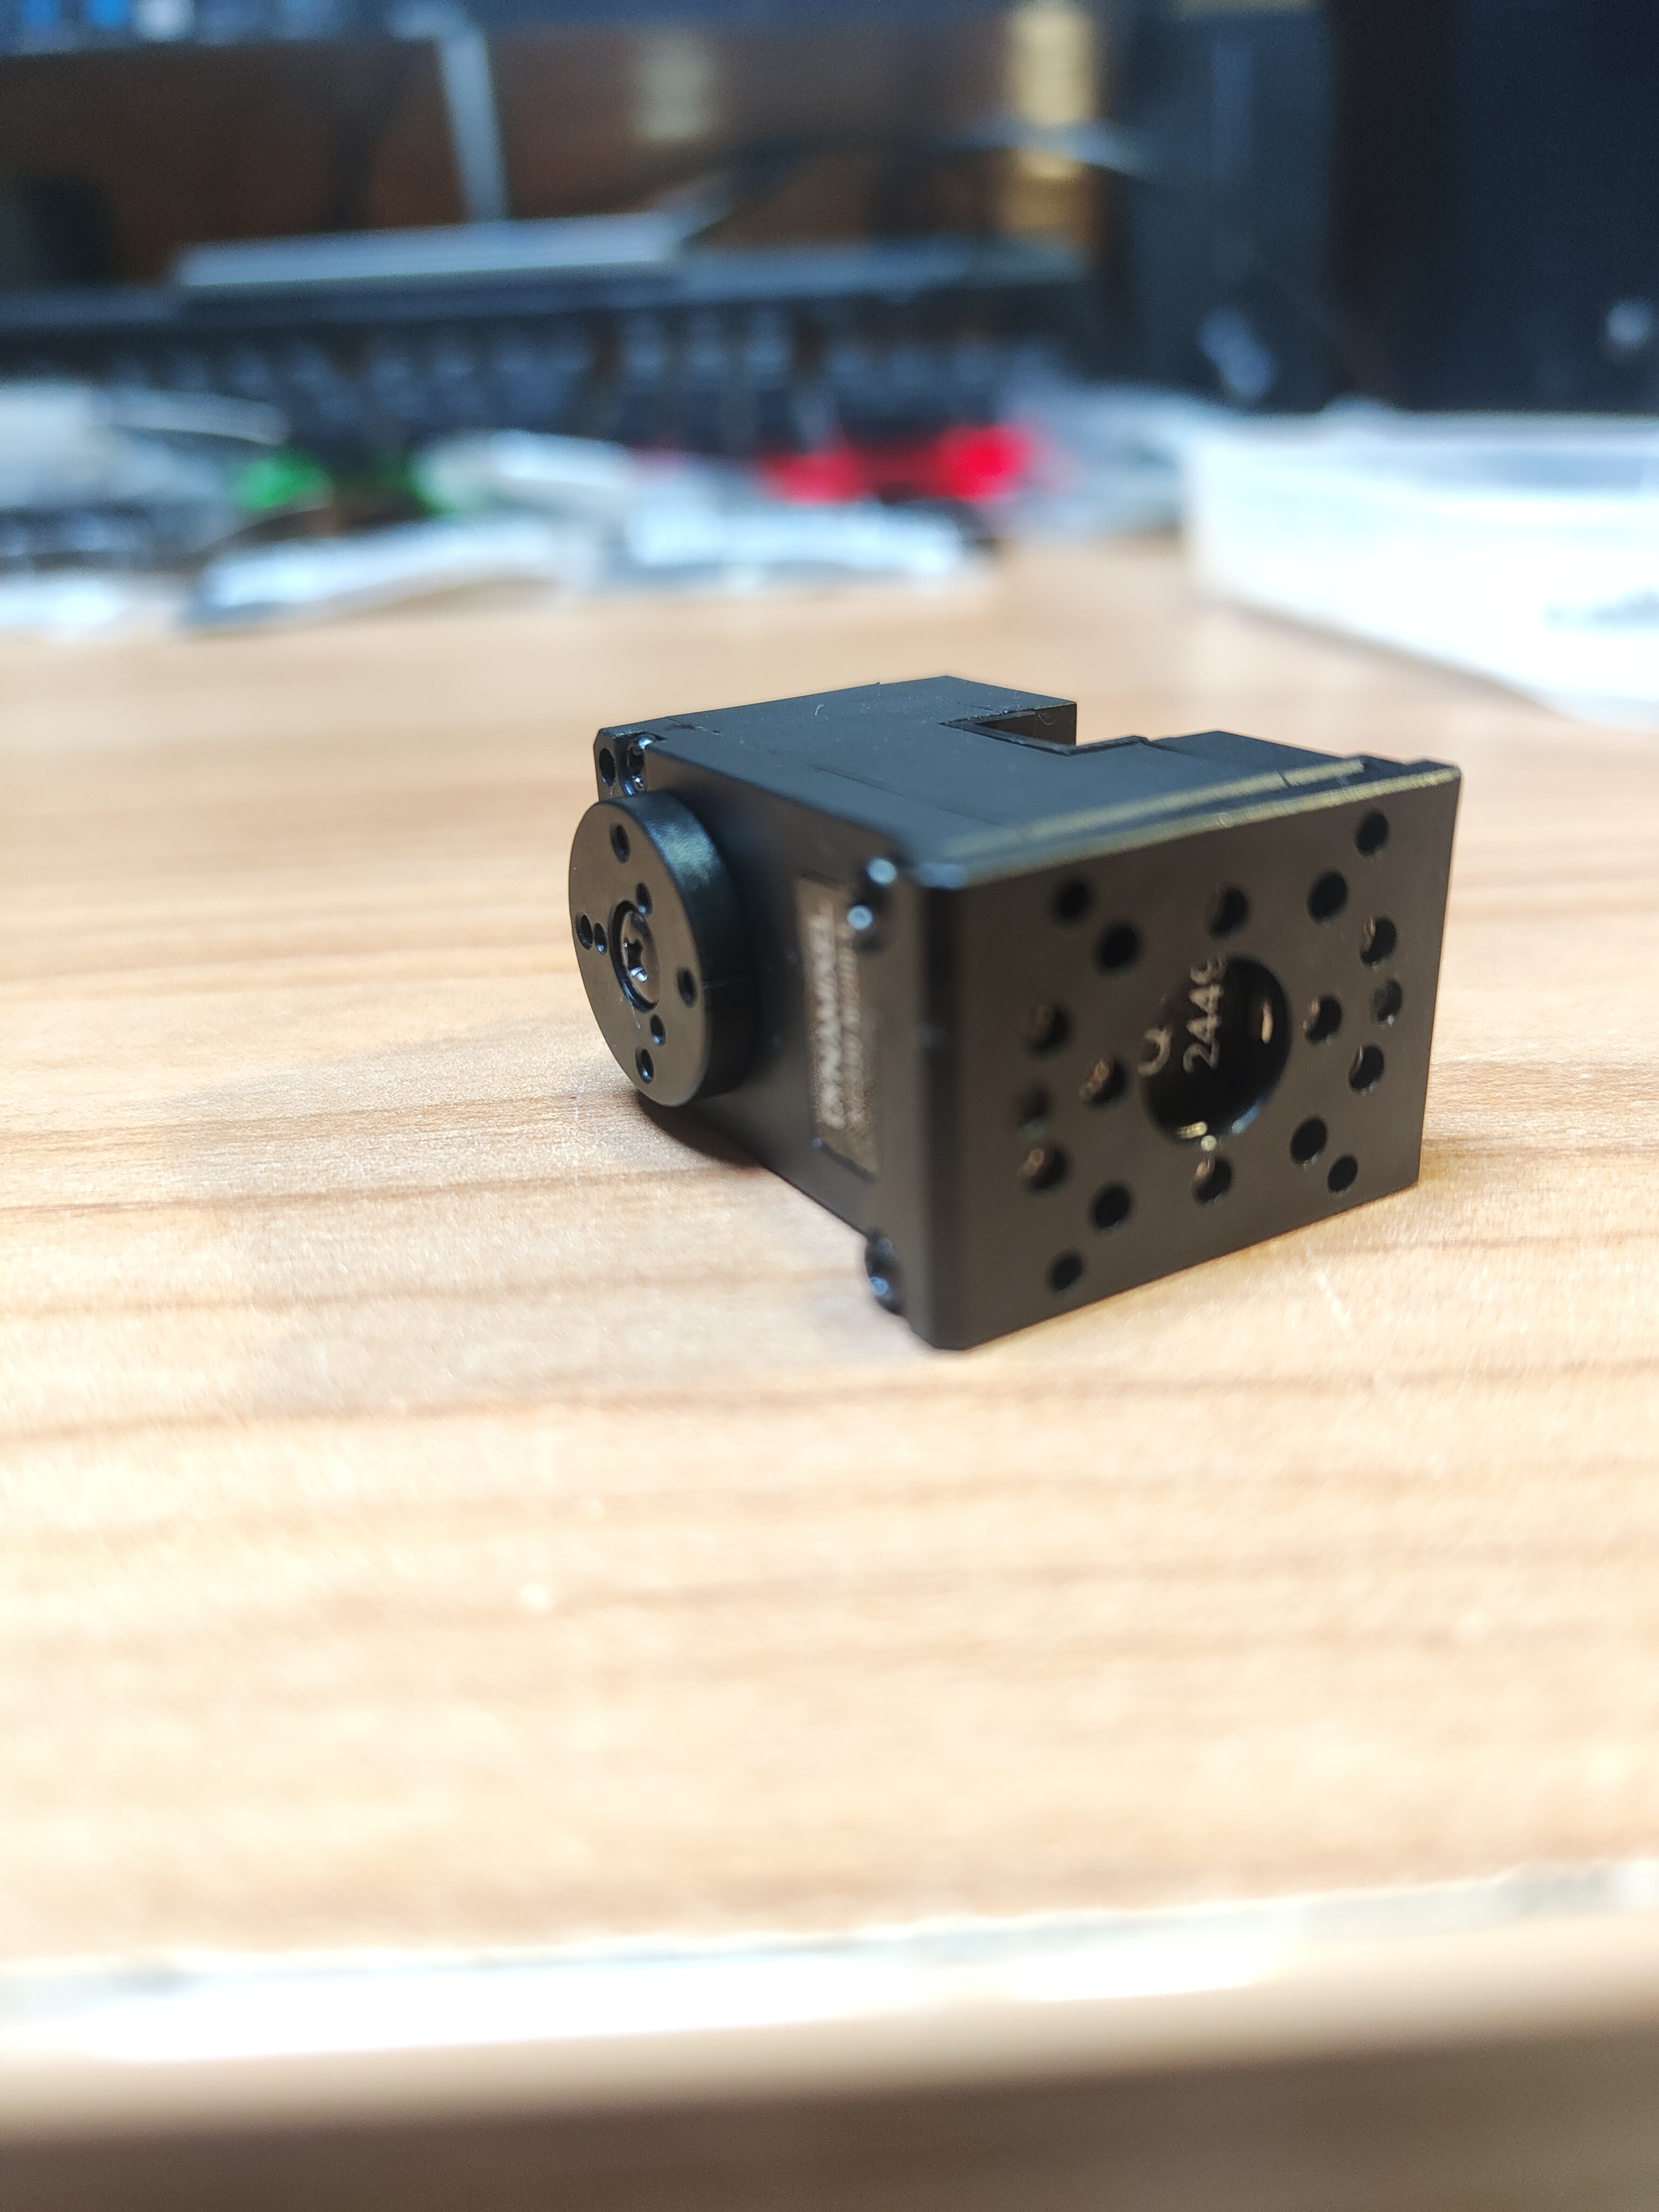
\includegraphics[width=0.25\textwidth]{figs/appendix/polegar/1.jpg} &
  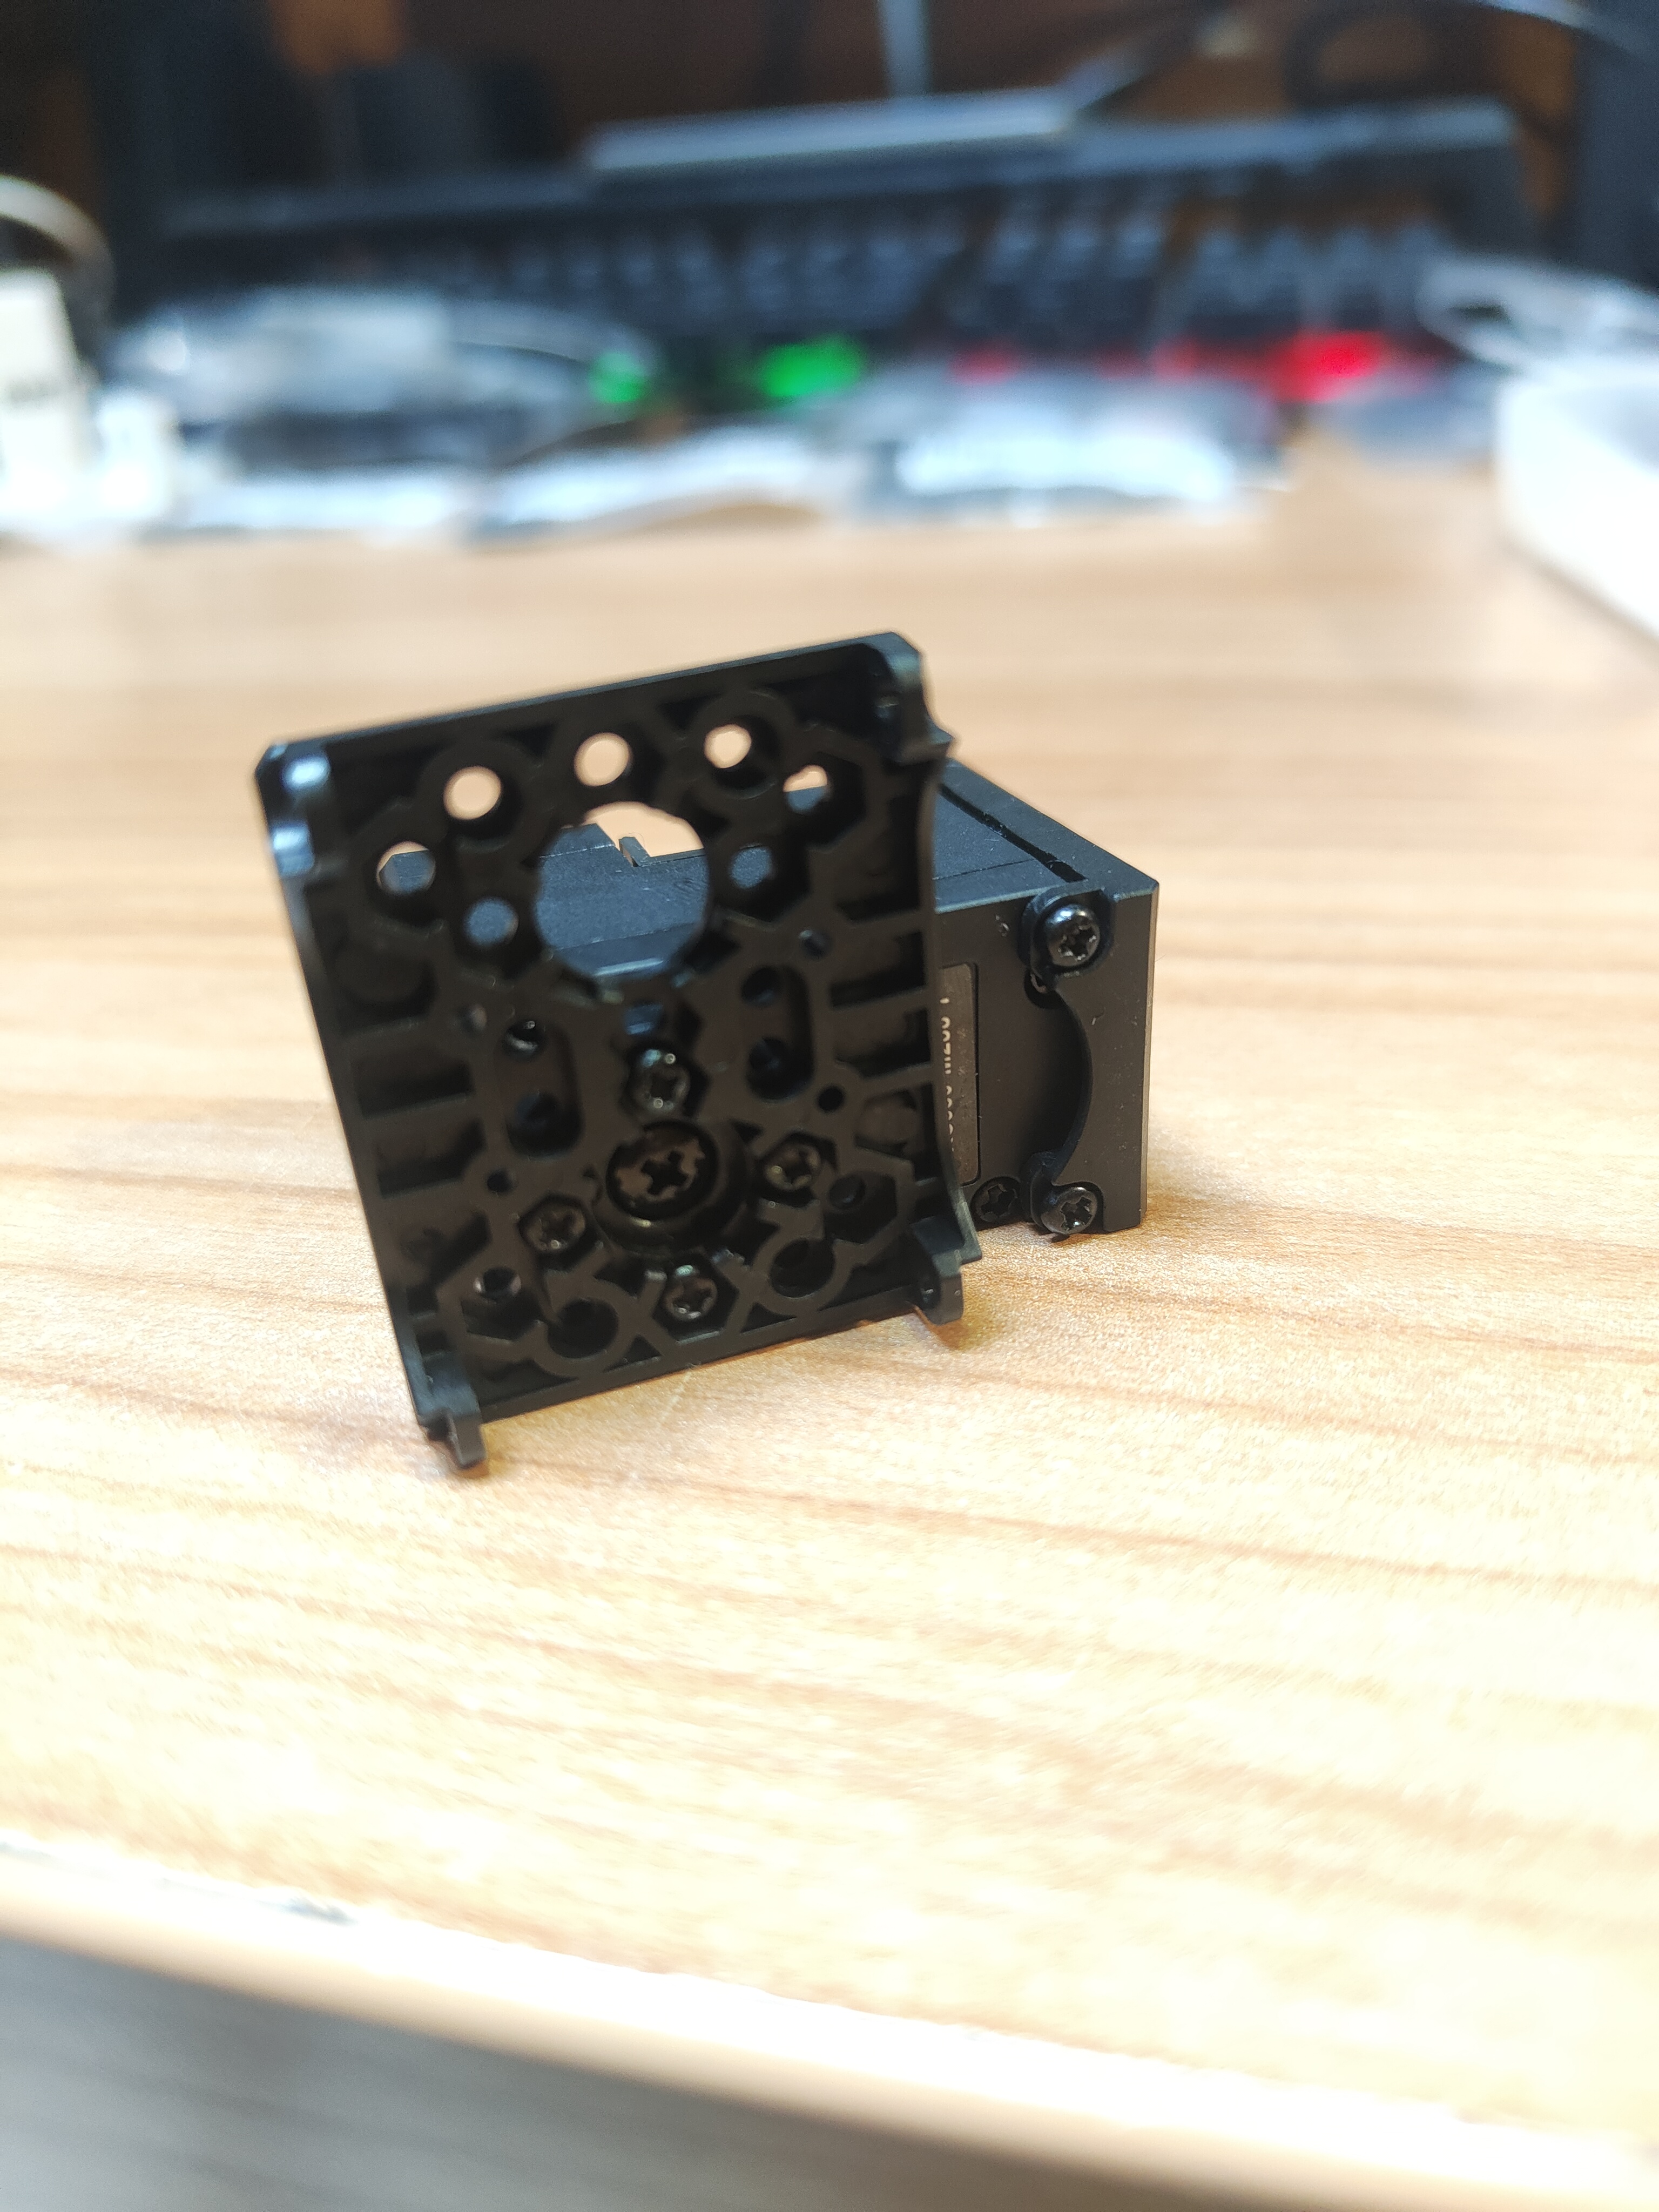
\includegraphics[width=0.25\textwidth]{figs/appendix/polegar/2.jpg} &
  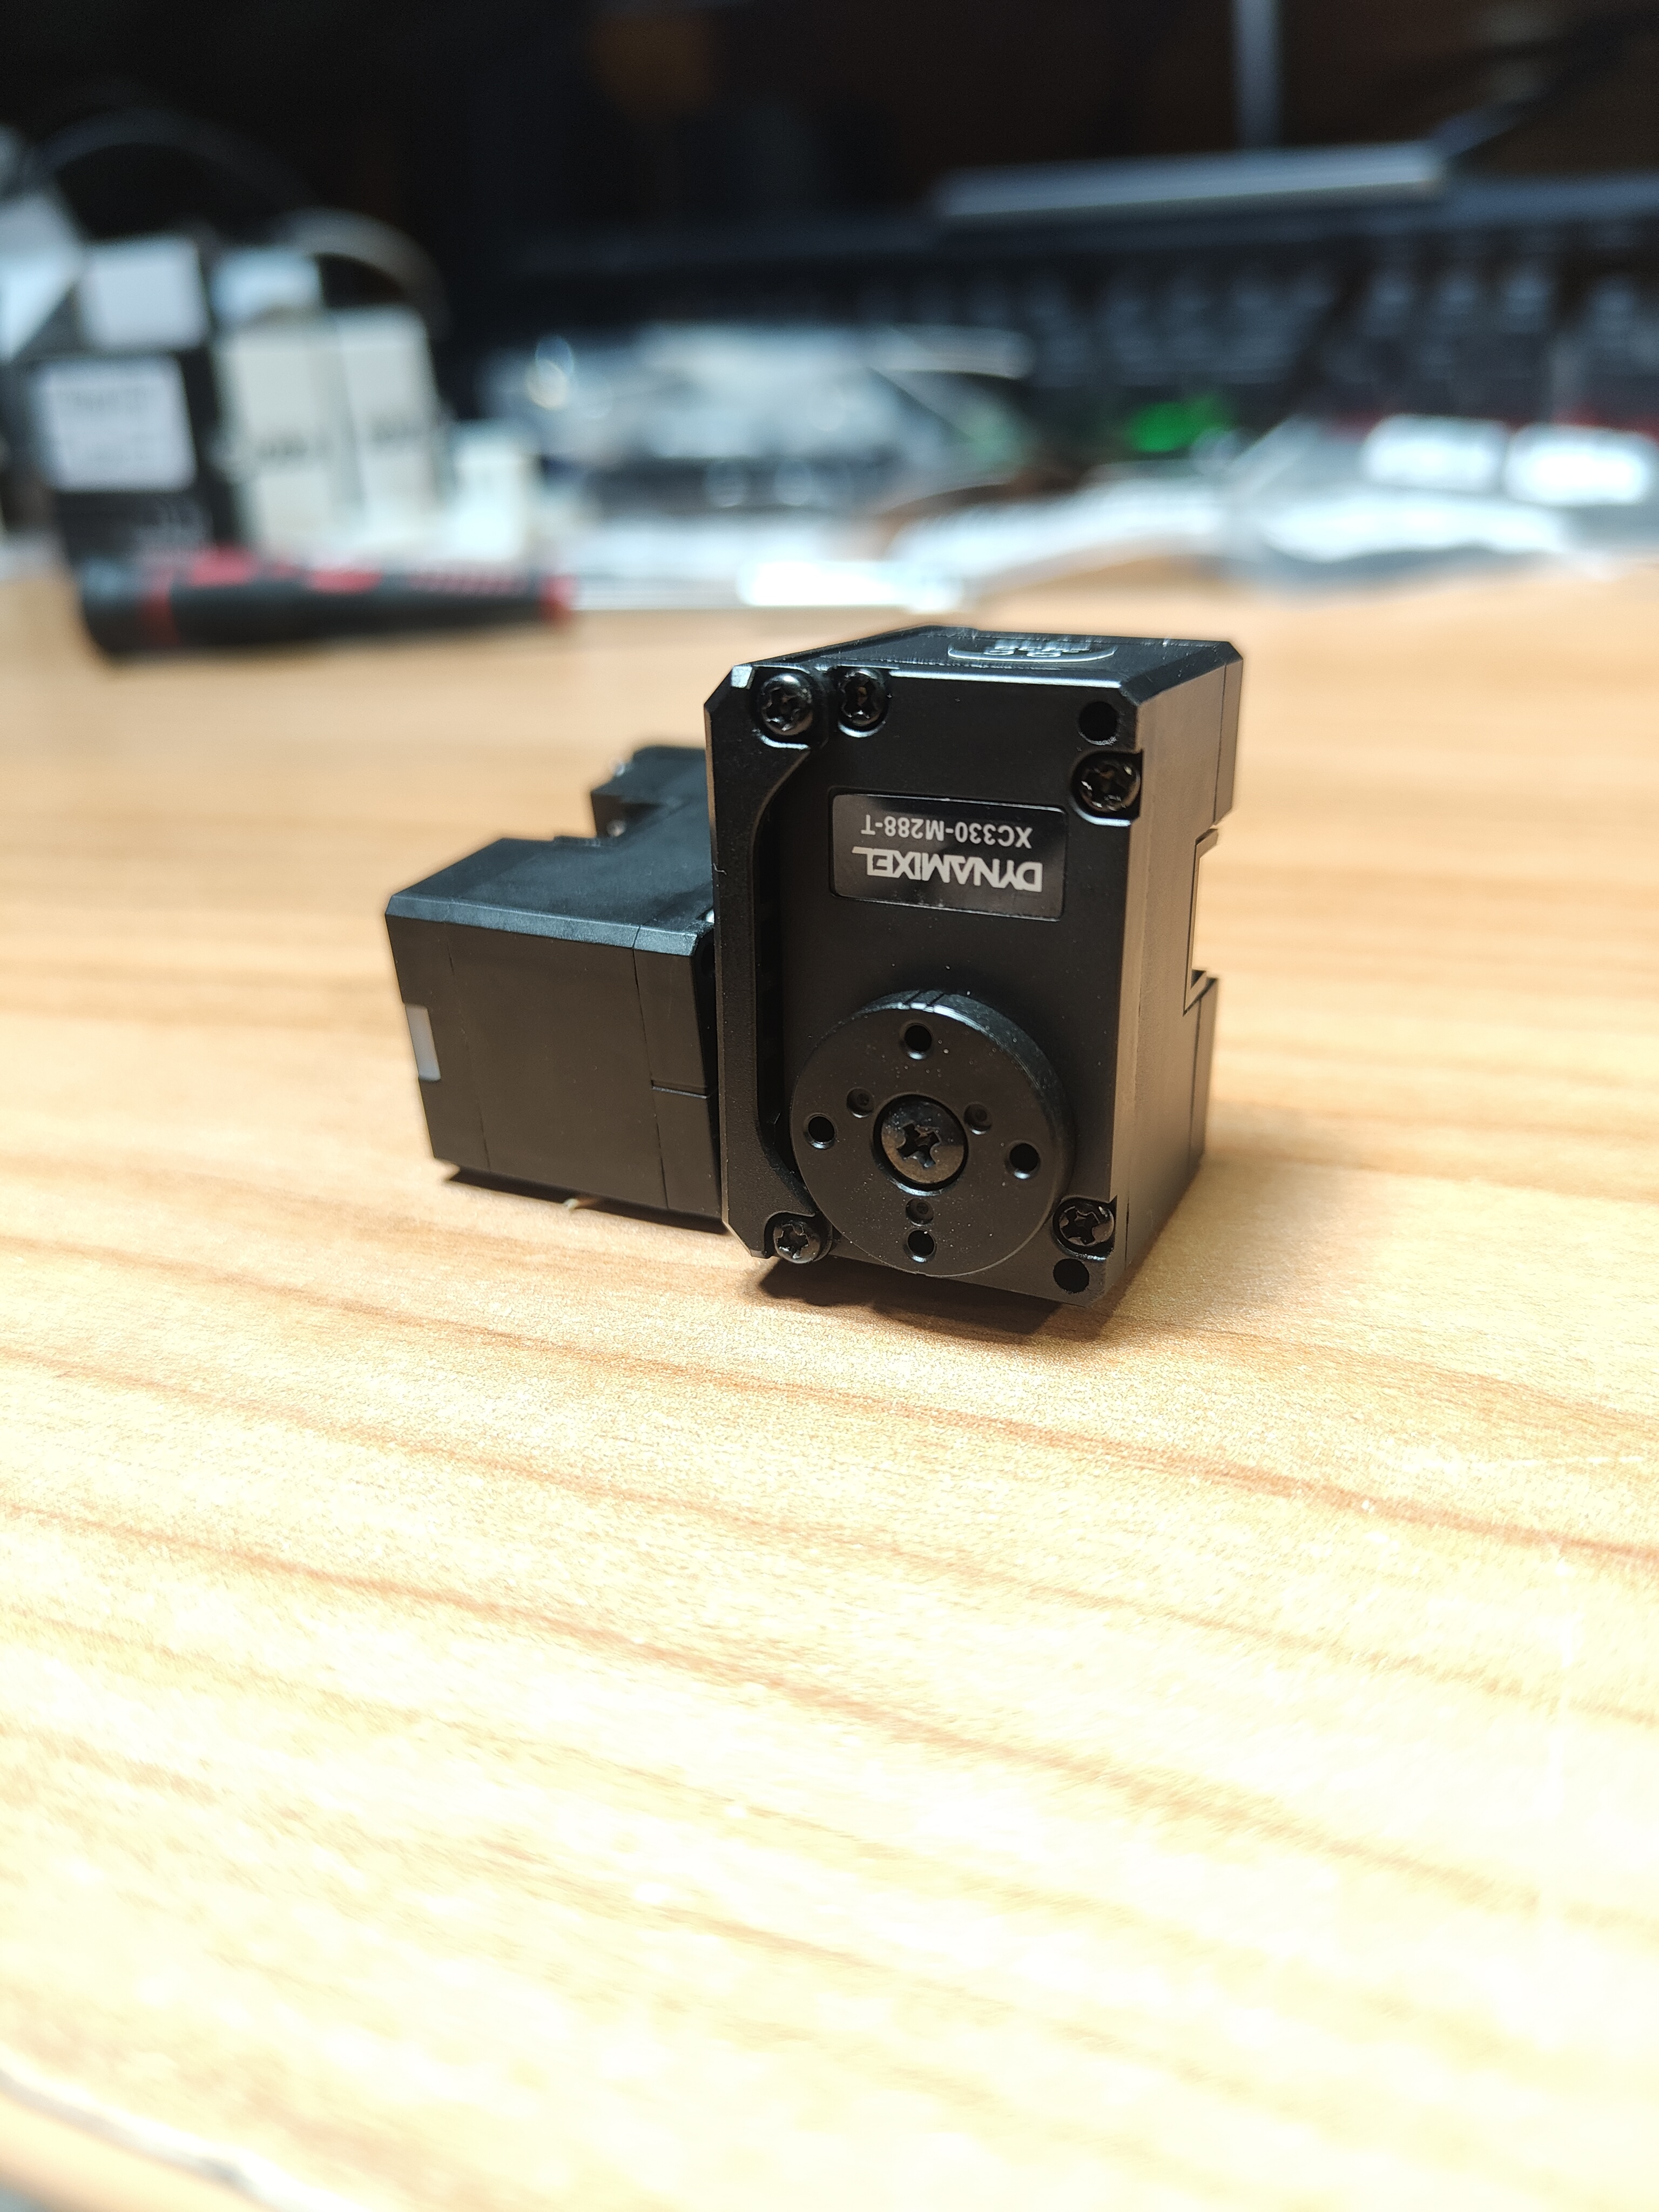
\includegraphics[width=0.25\textwidth]{figs/appendix/polegar/3.jpg} \\
  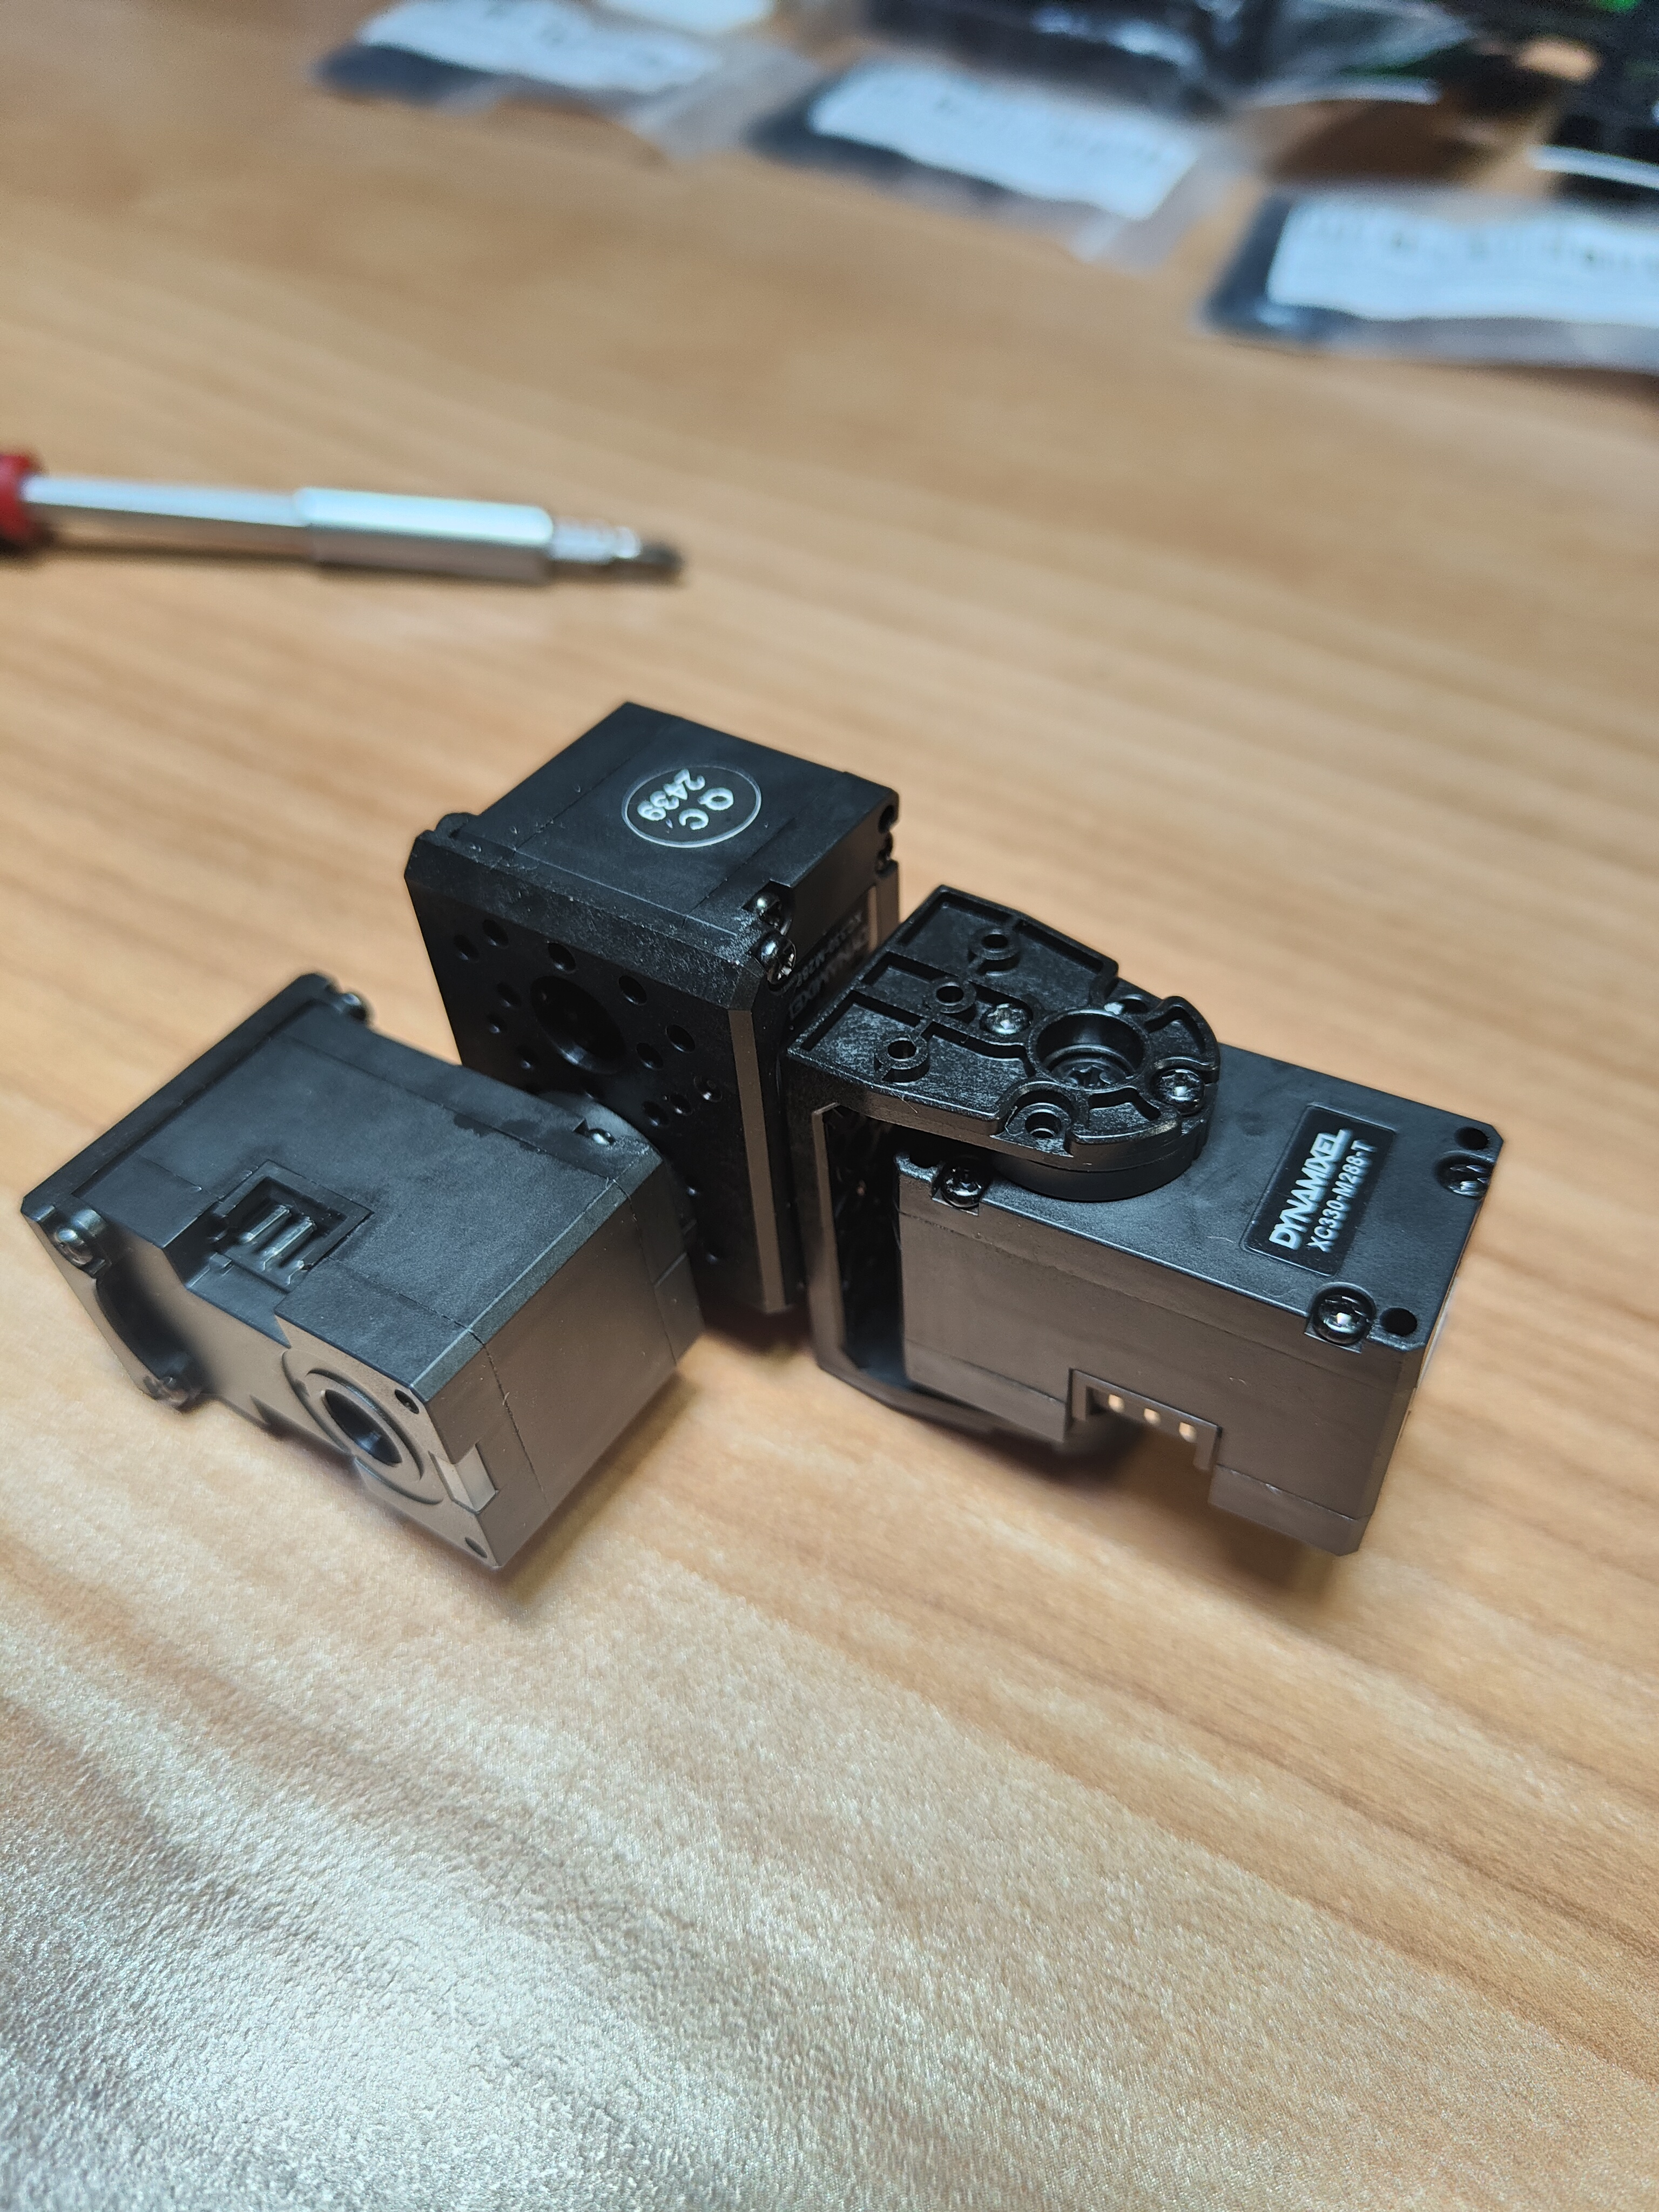
\includegraphics[width=0.25\textwidth]{figs/appendix/polegar/4.jpg} &
  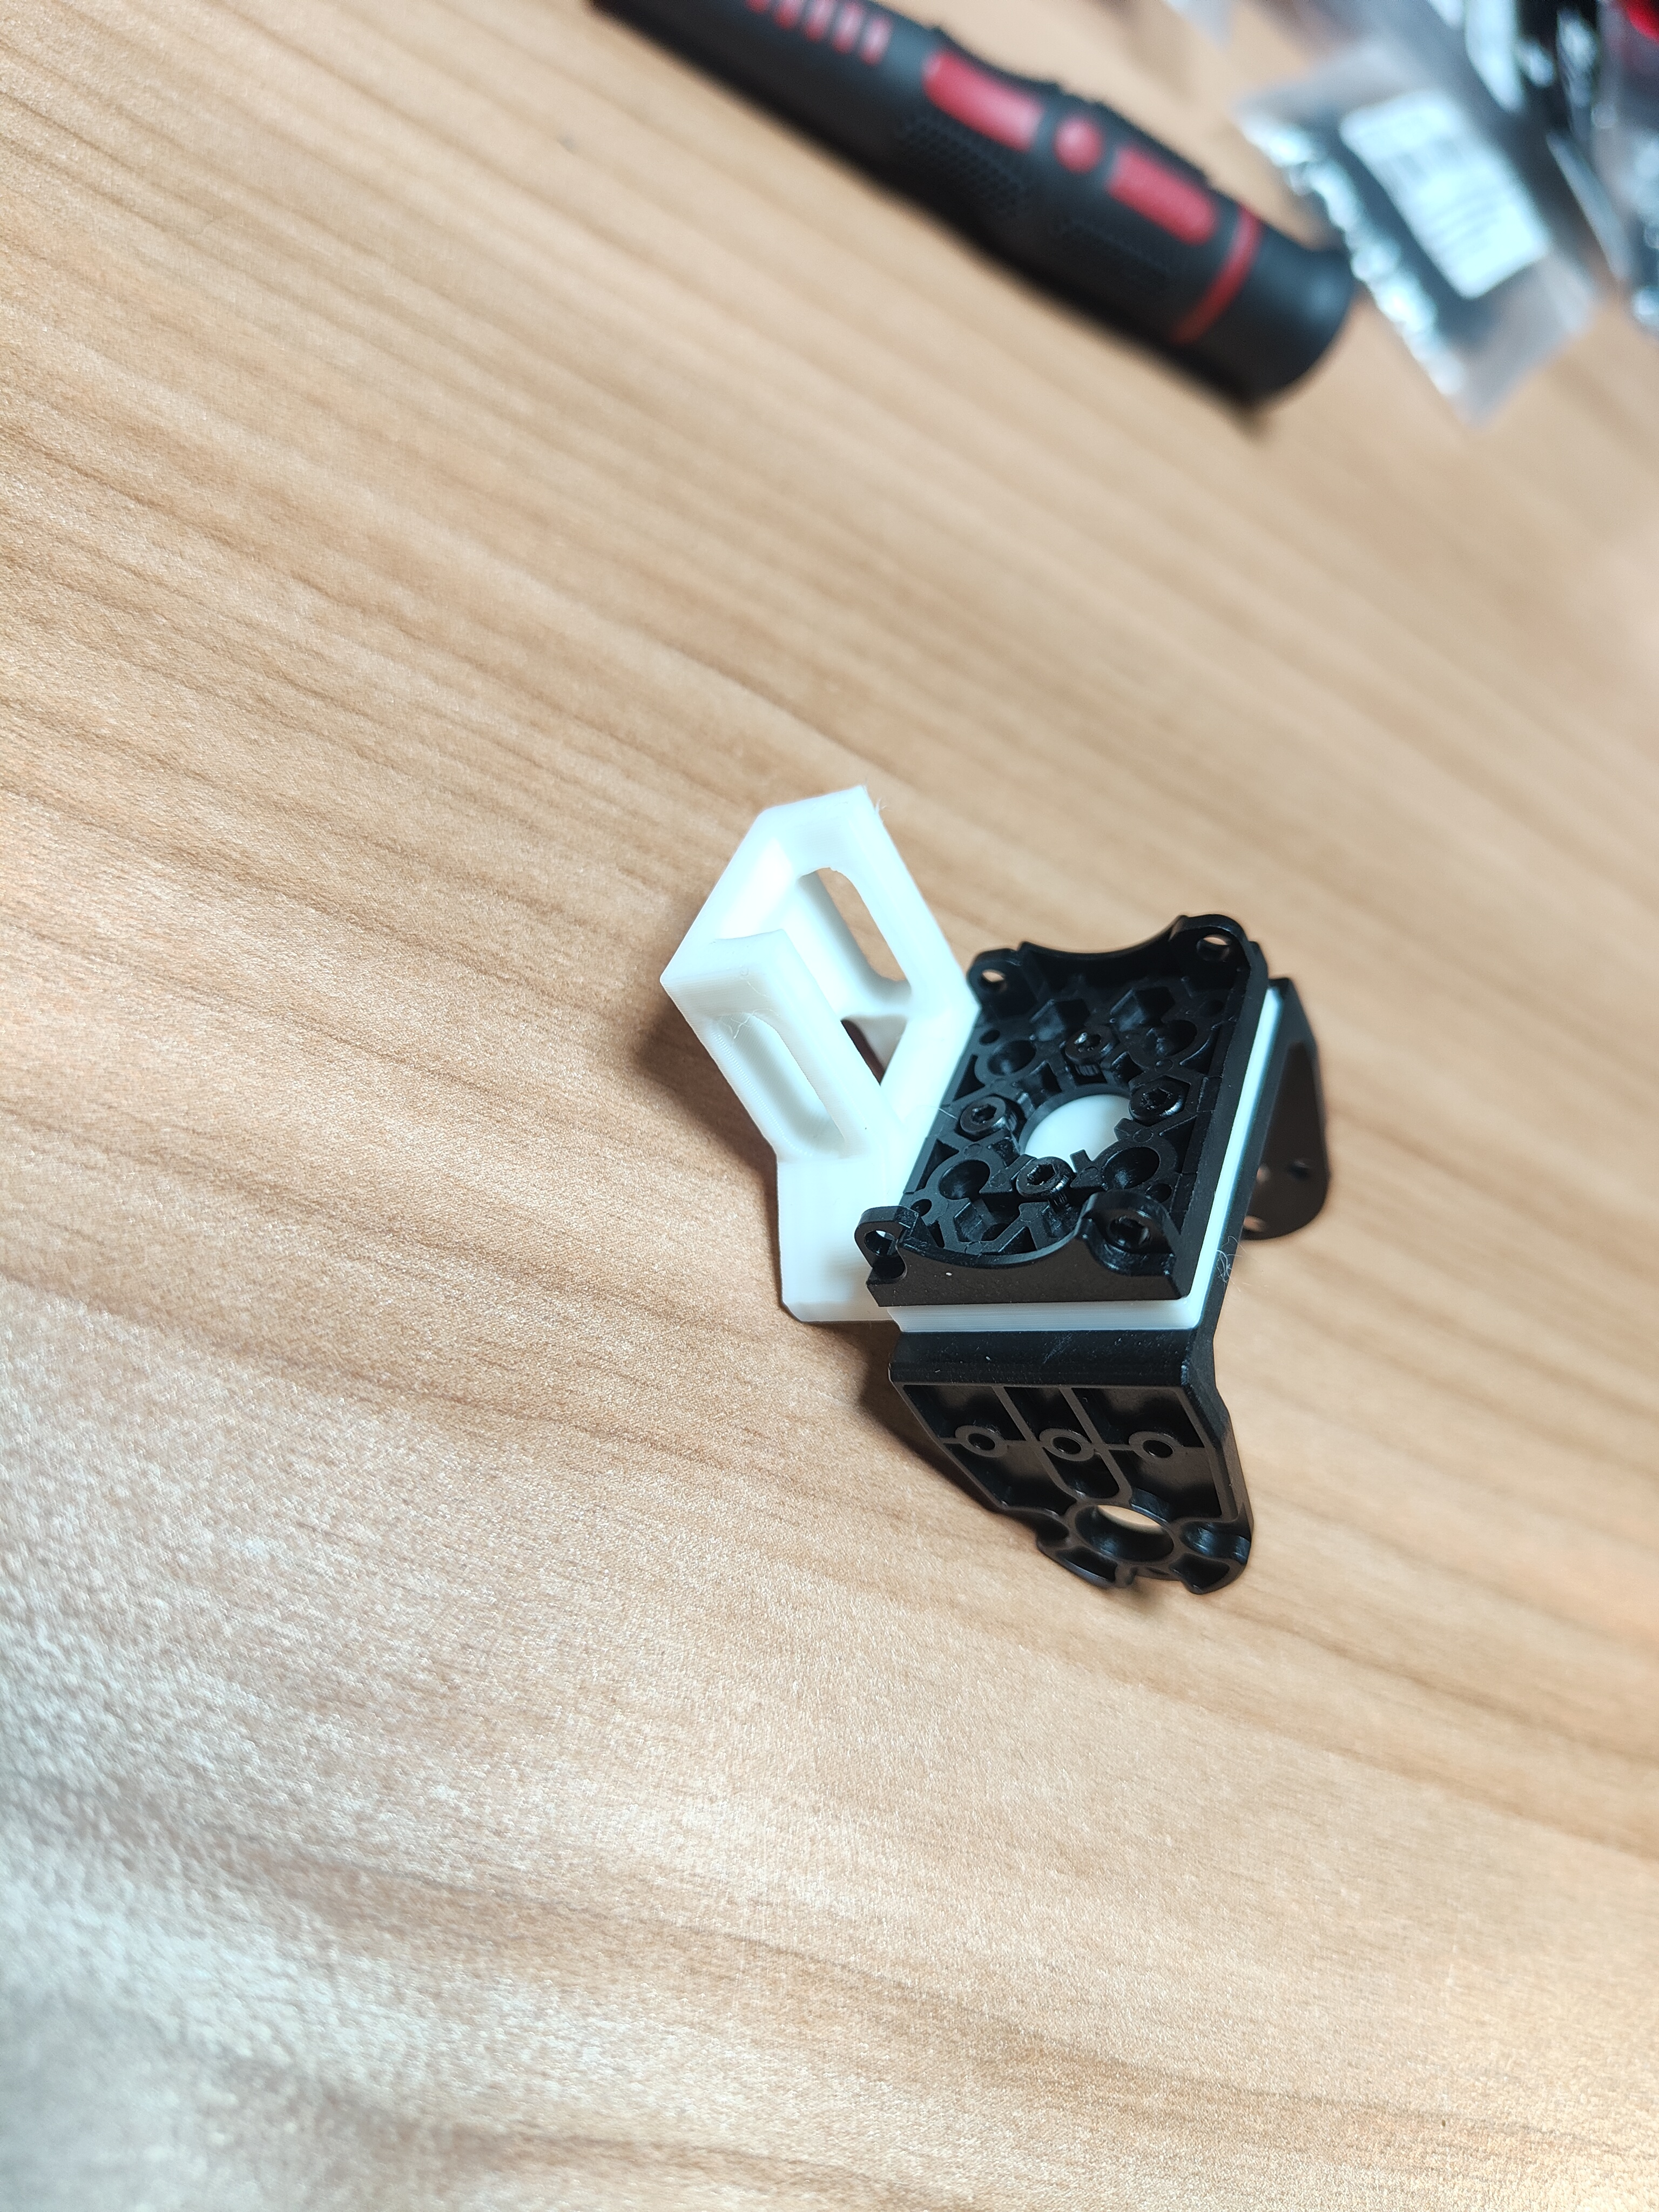
\includegraphics[width=0.25\textwidth]{figs/appendix/polegar/5.jpg} &
  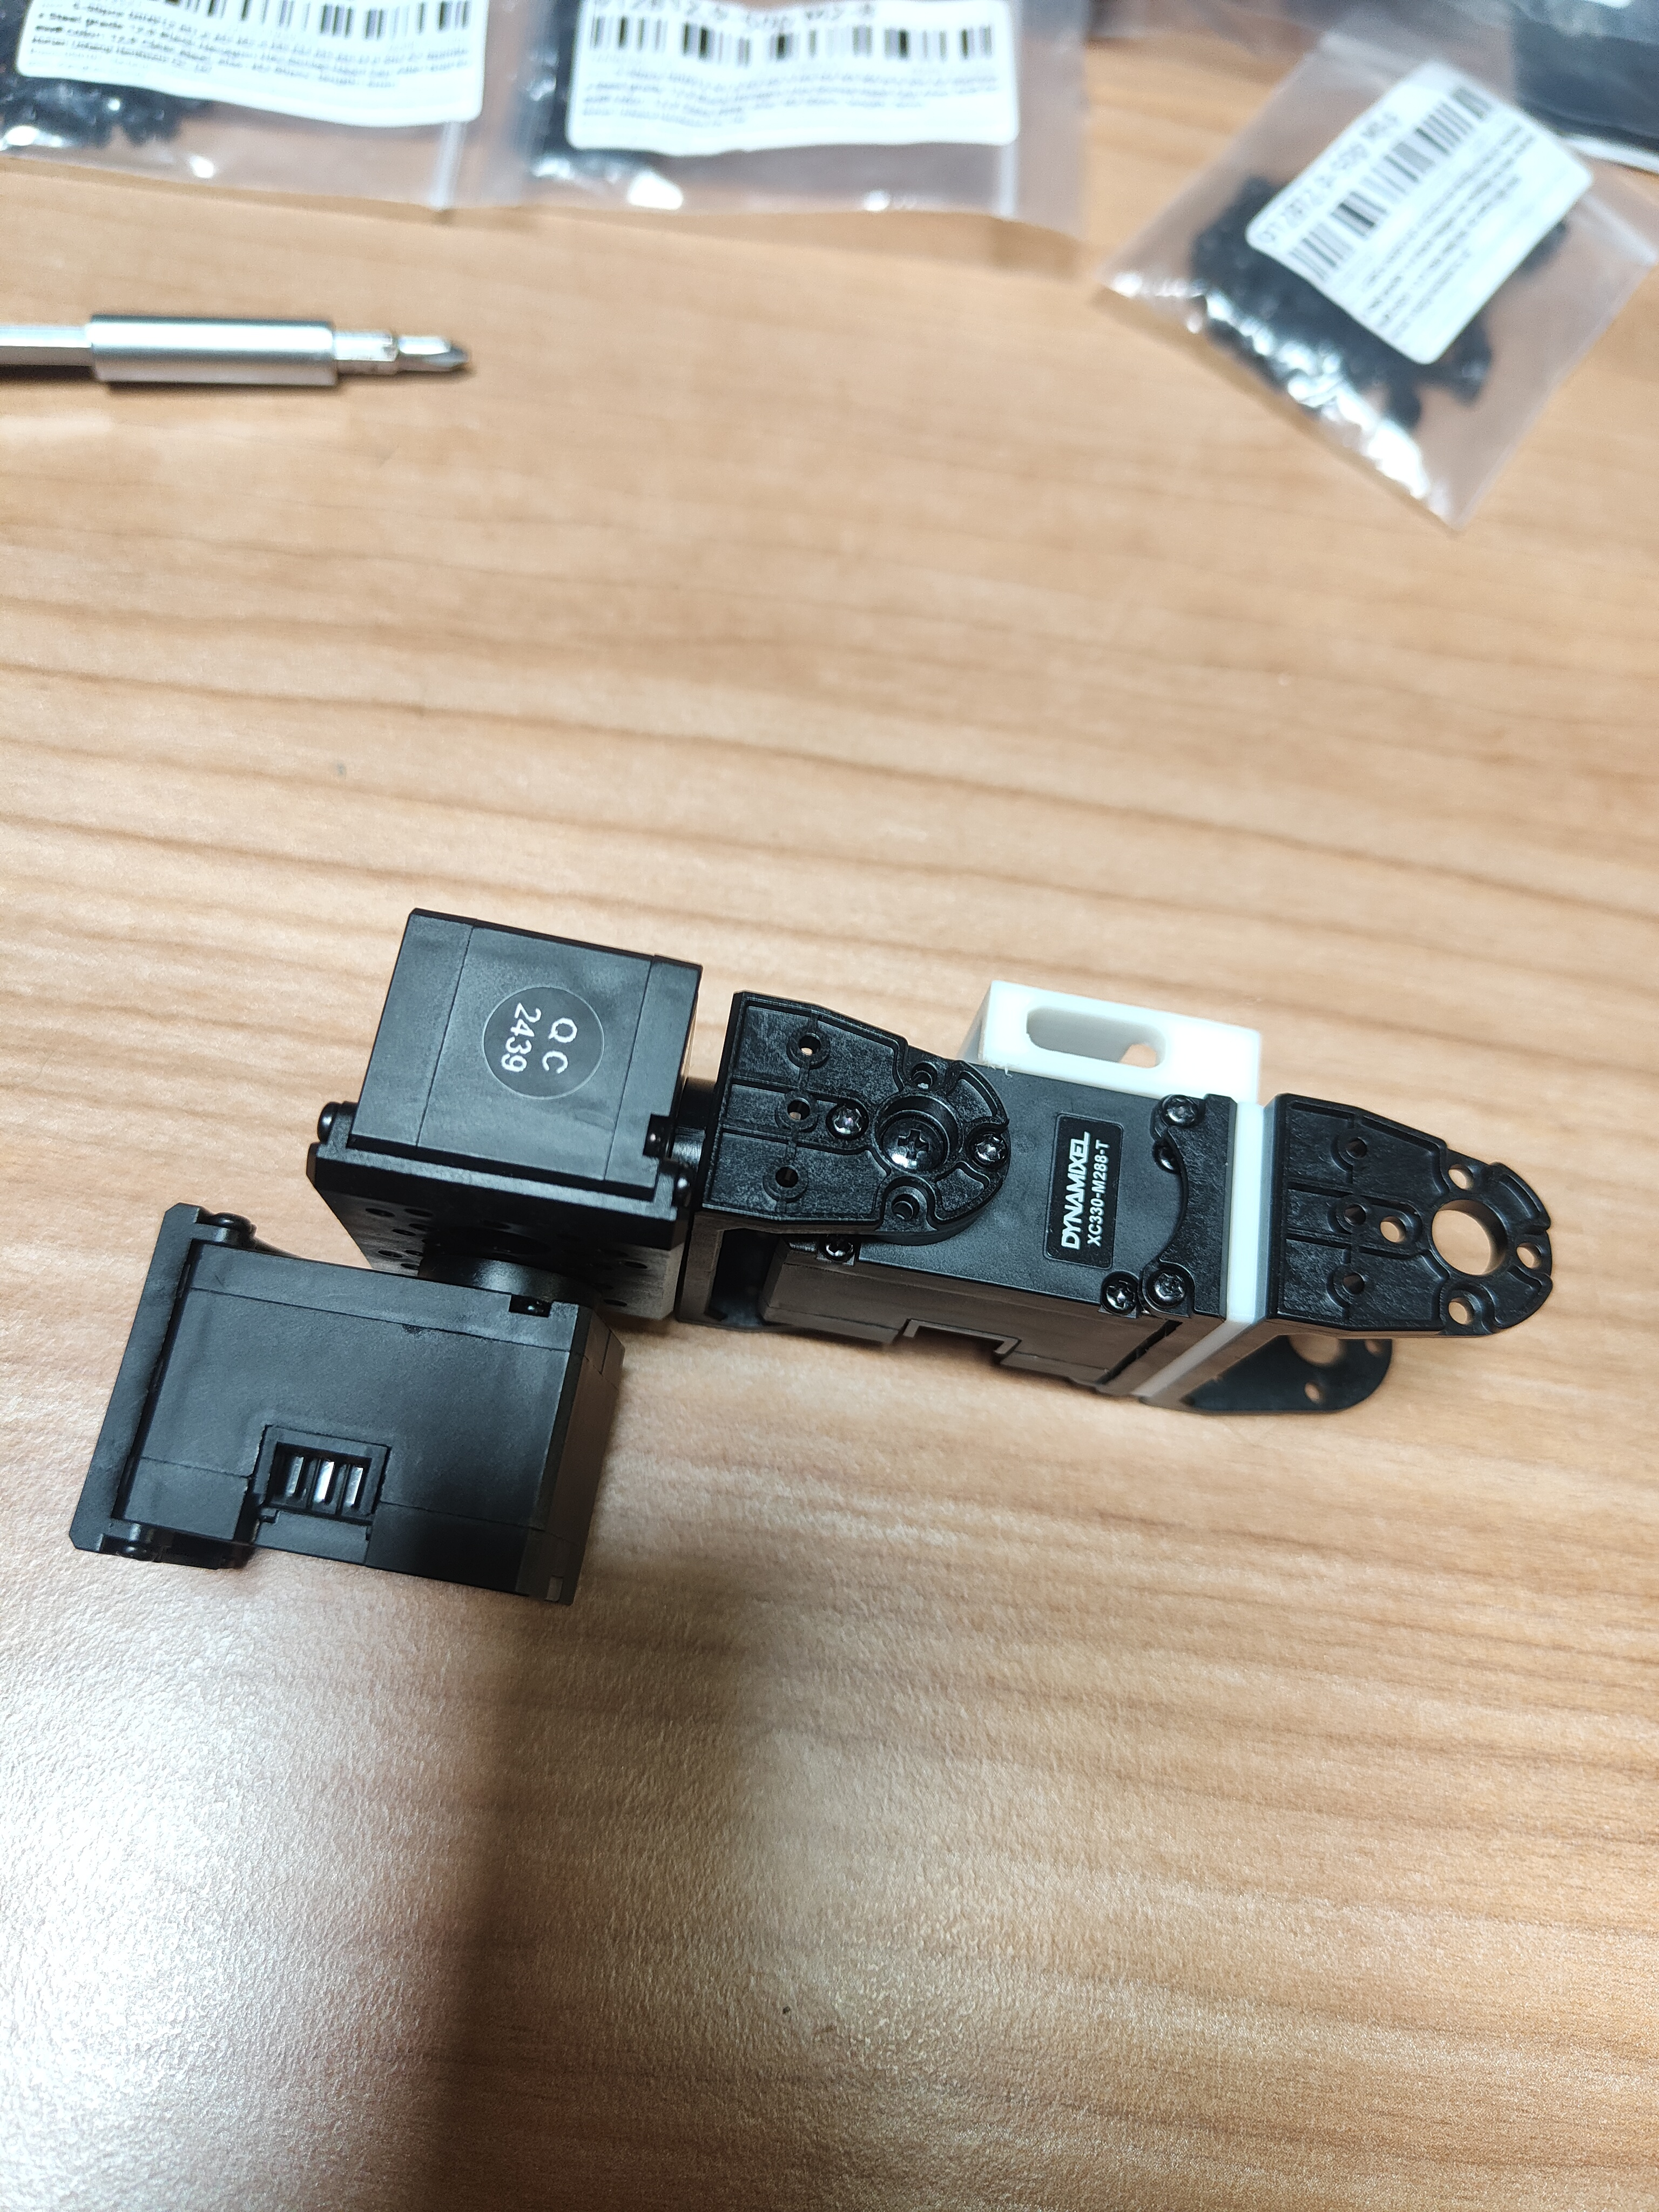
\includegraphics[width=0.25\textwidth]{figs/appendix/polegar/6.jpg} \\
  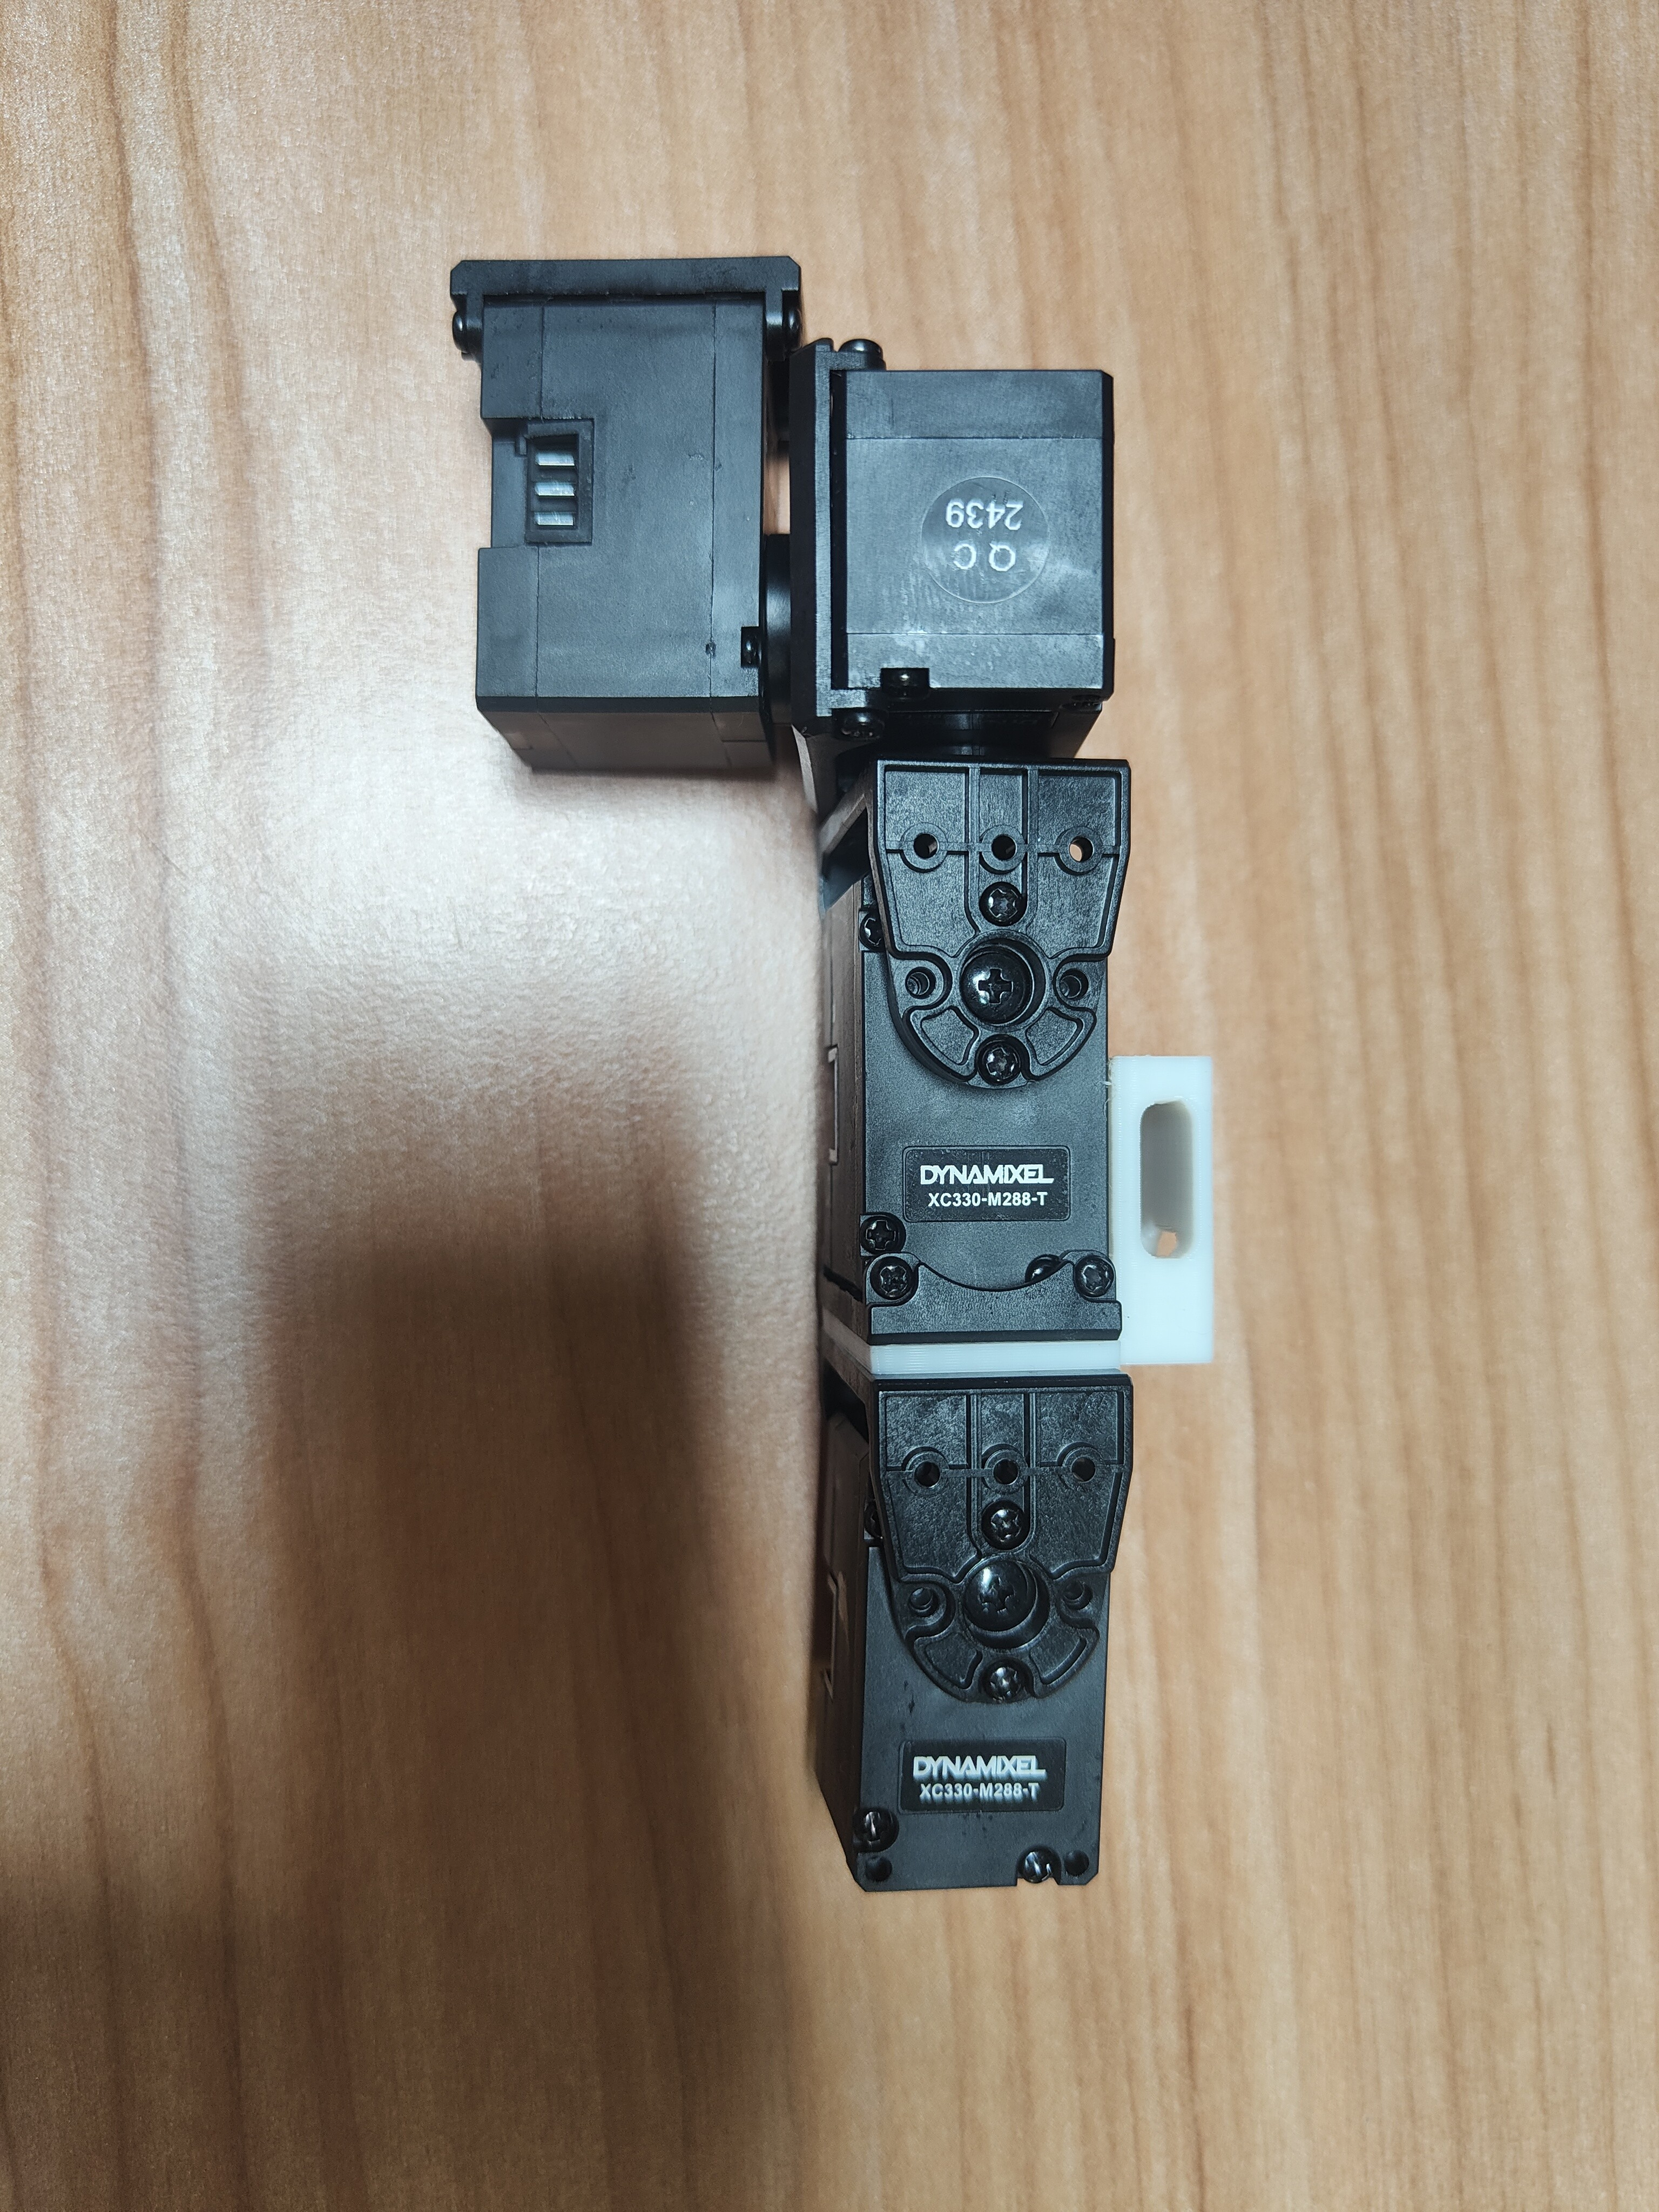
\includegraphics[width=0.25\textwidth]{figs/appendix/polegar/7.jpg} &
  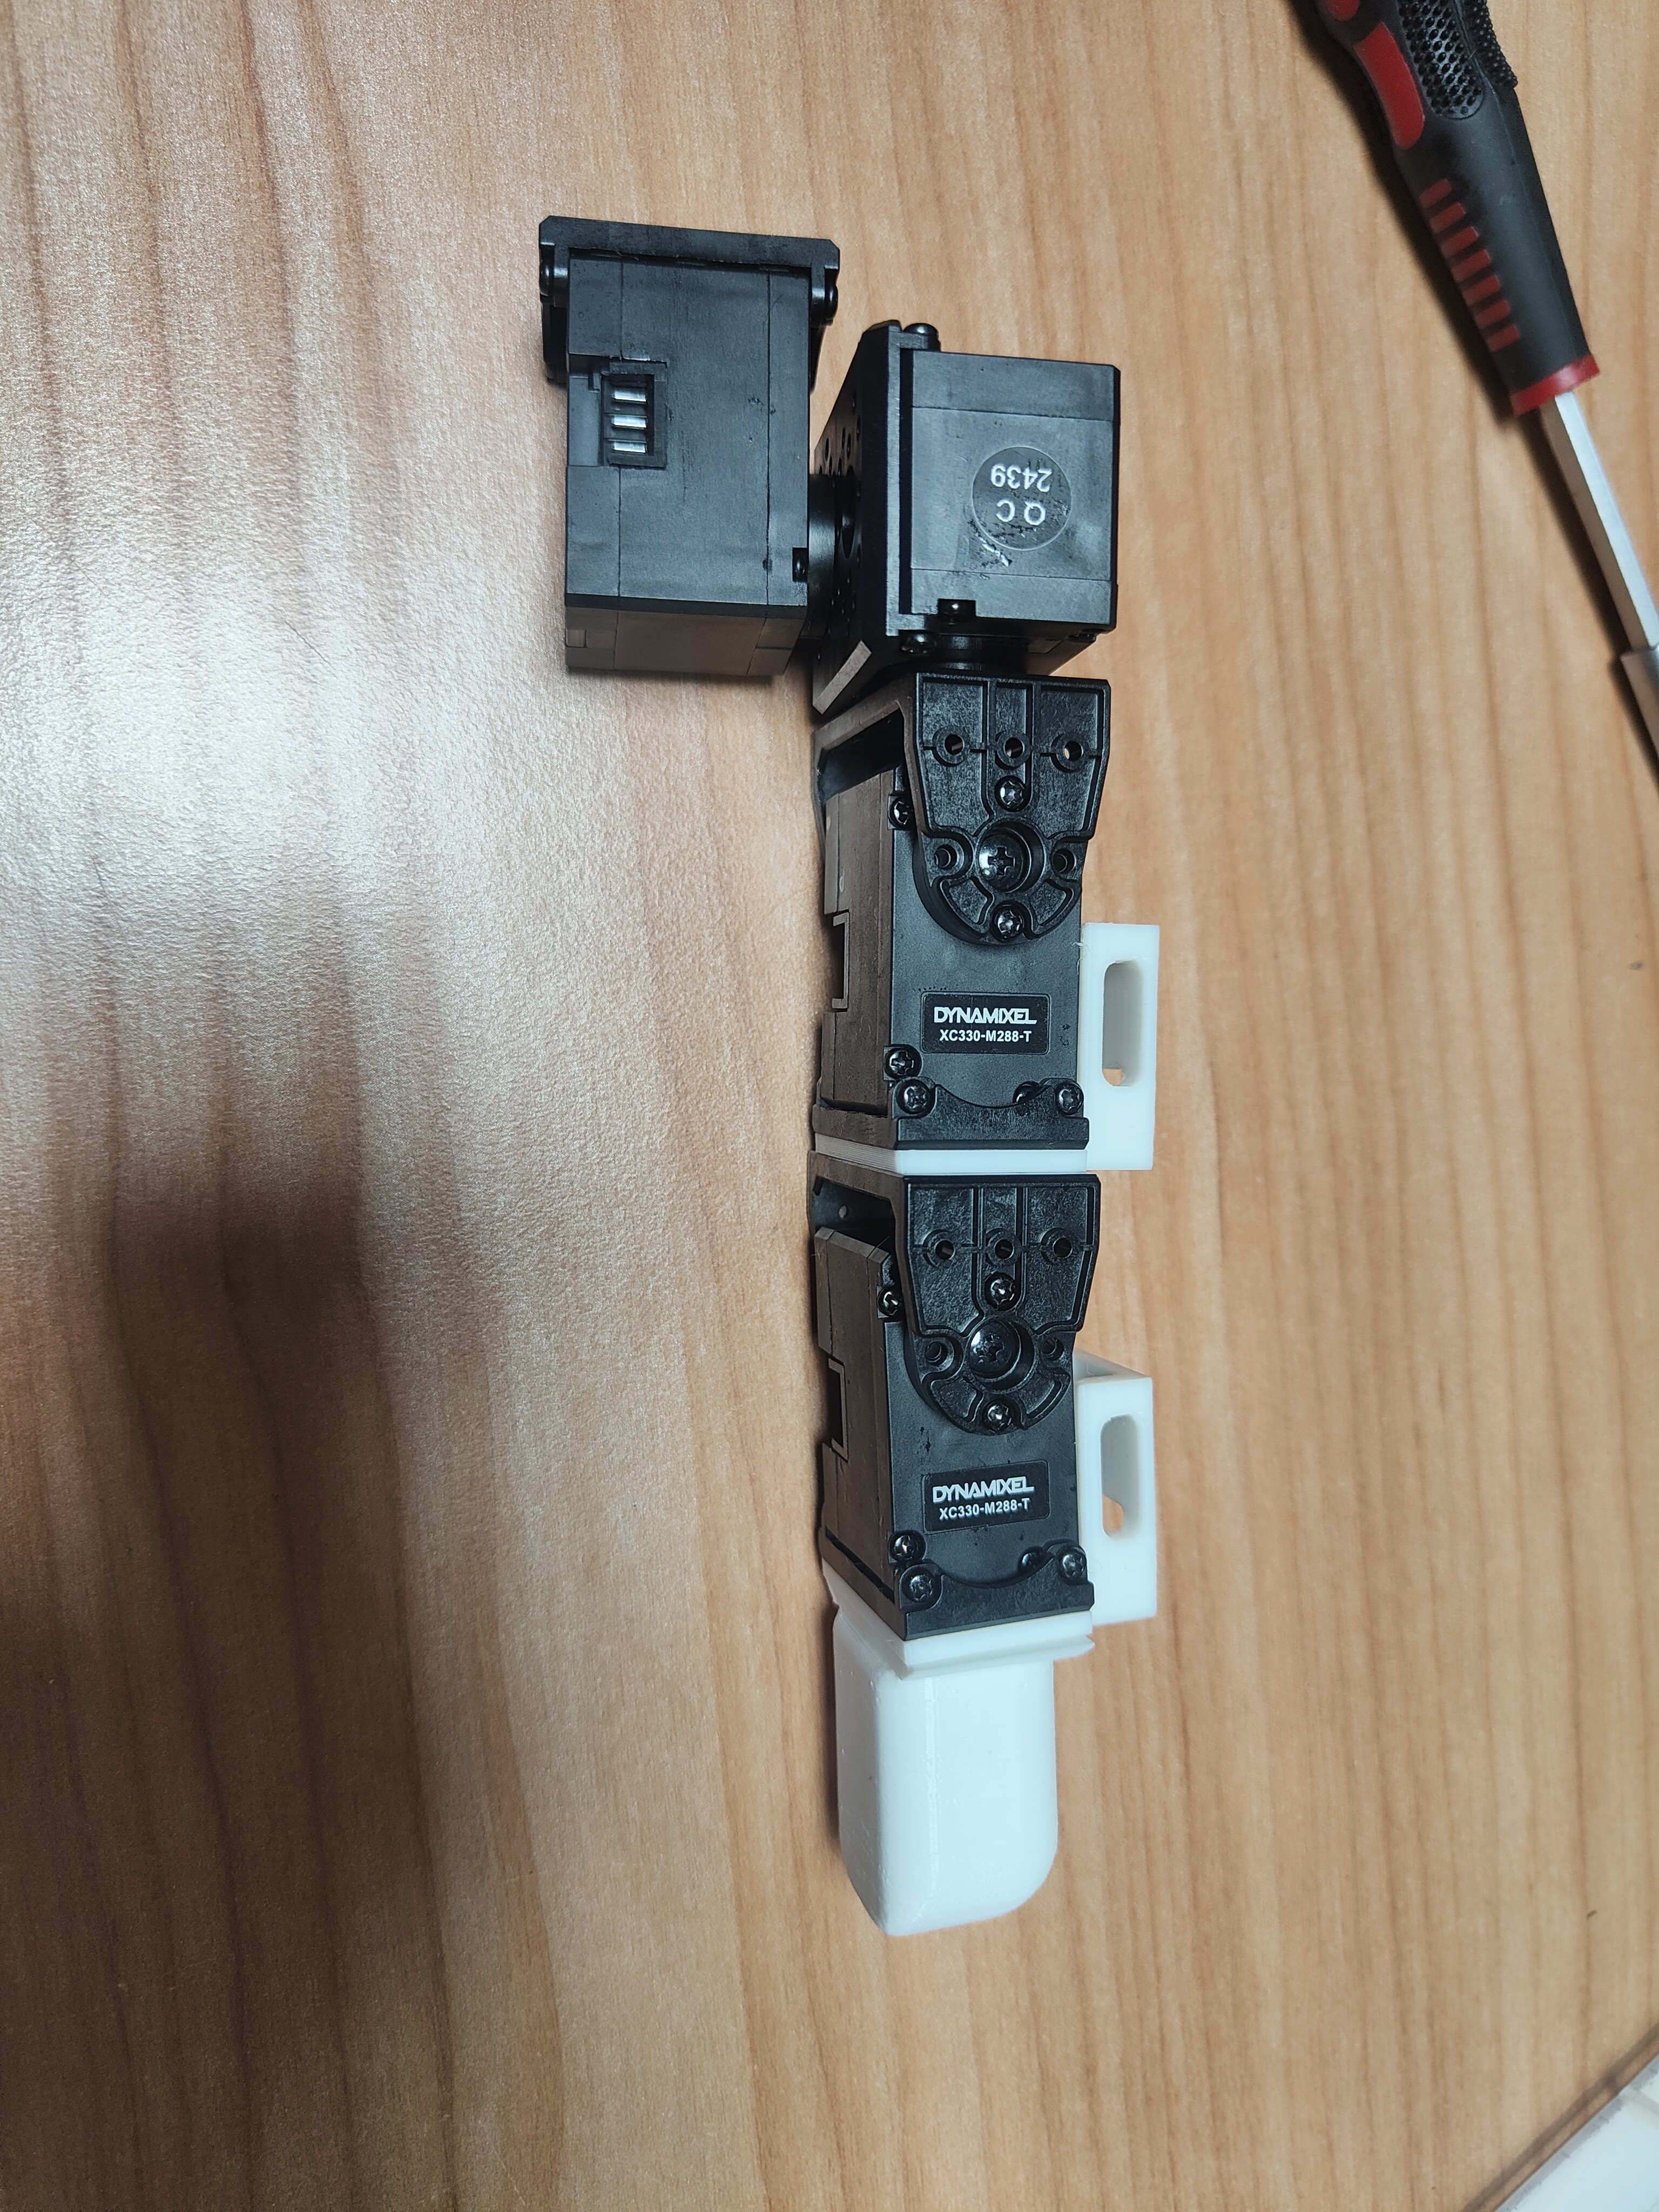
\includegraphics[width=0.25\textwidth]{figs/appendix/polegar/8.jpg} &
  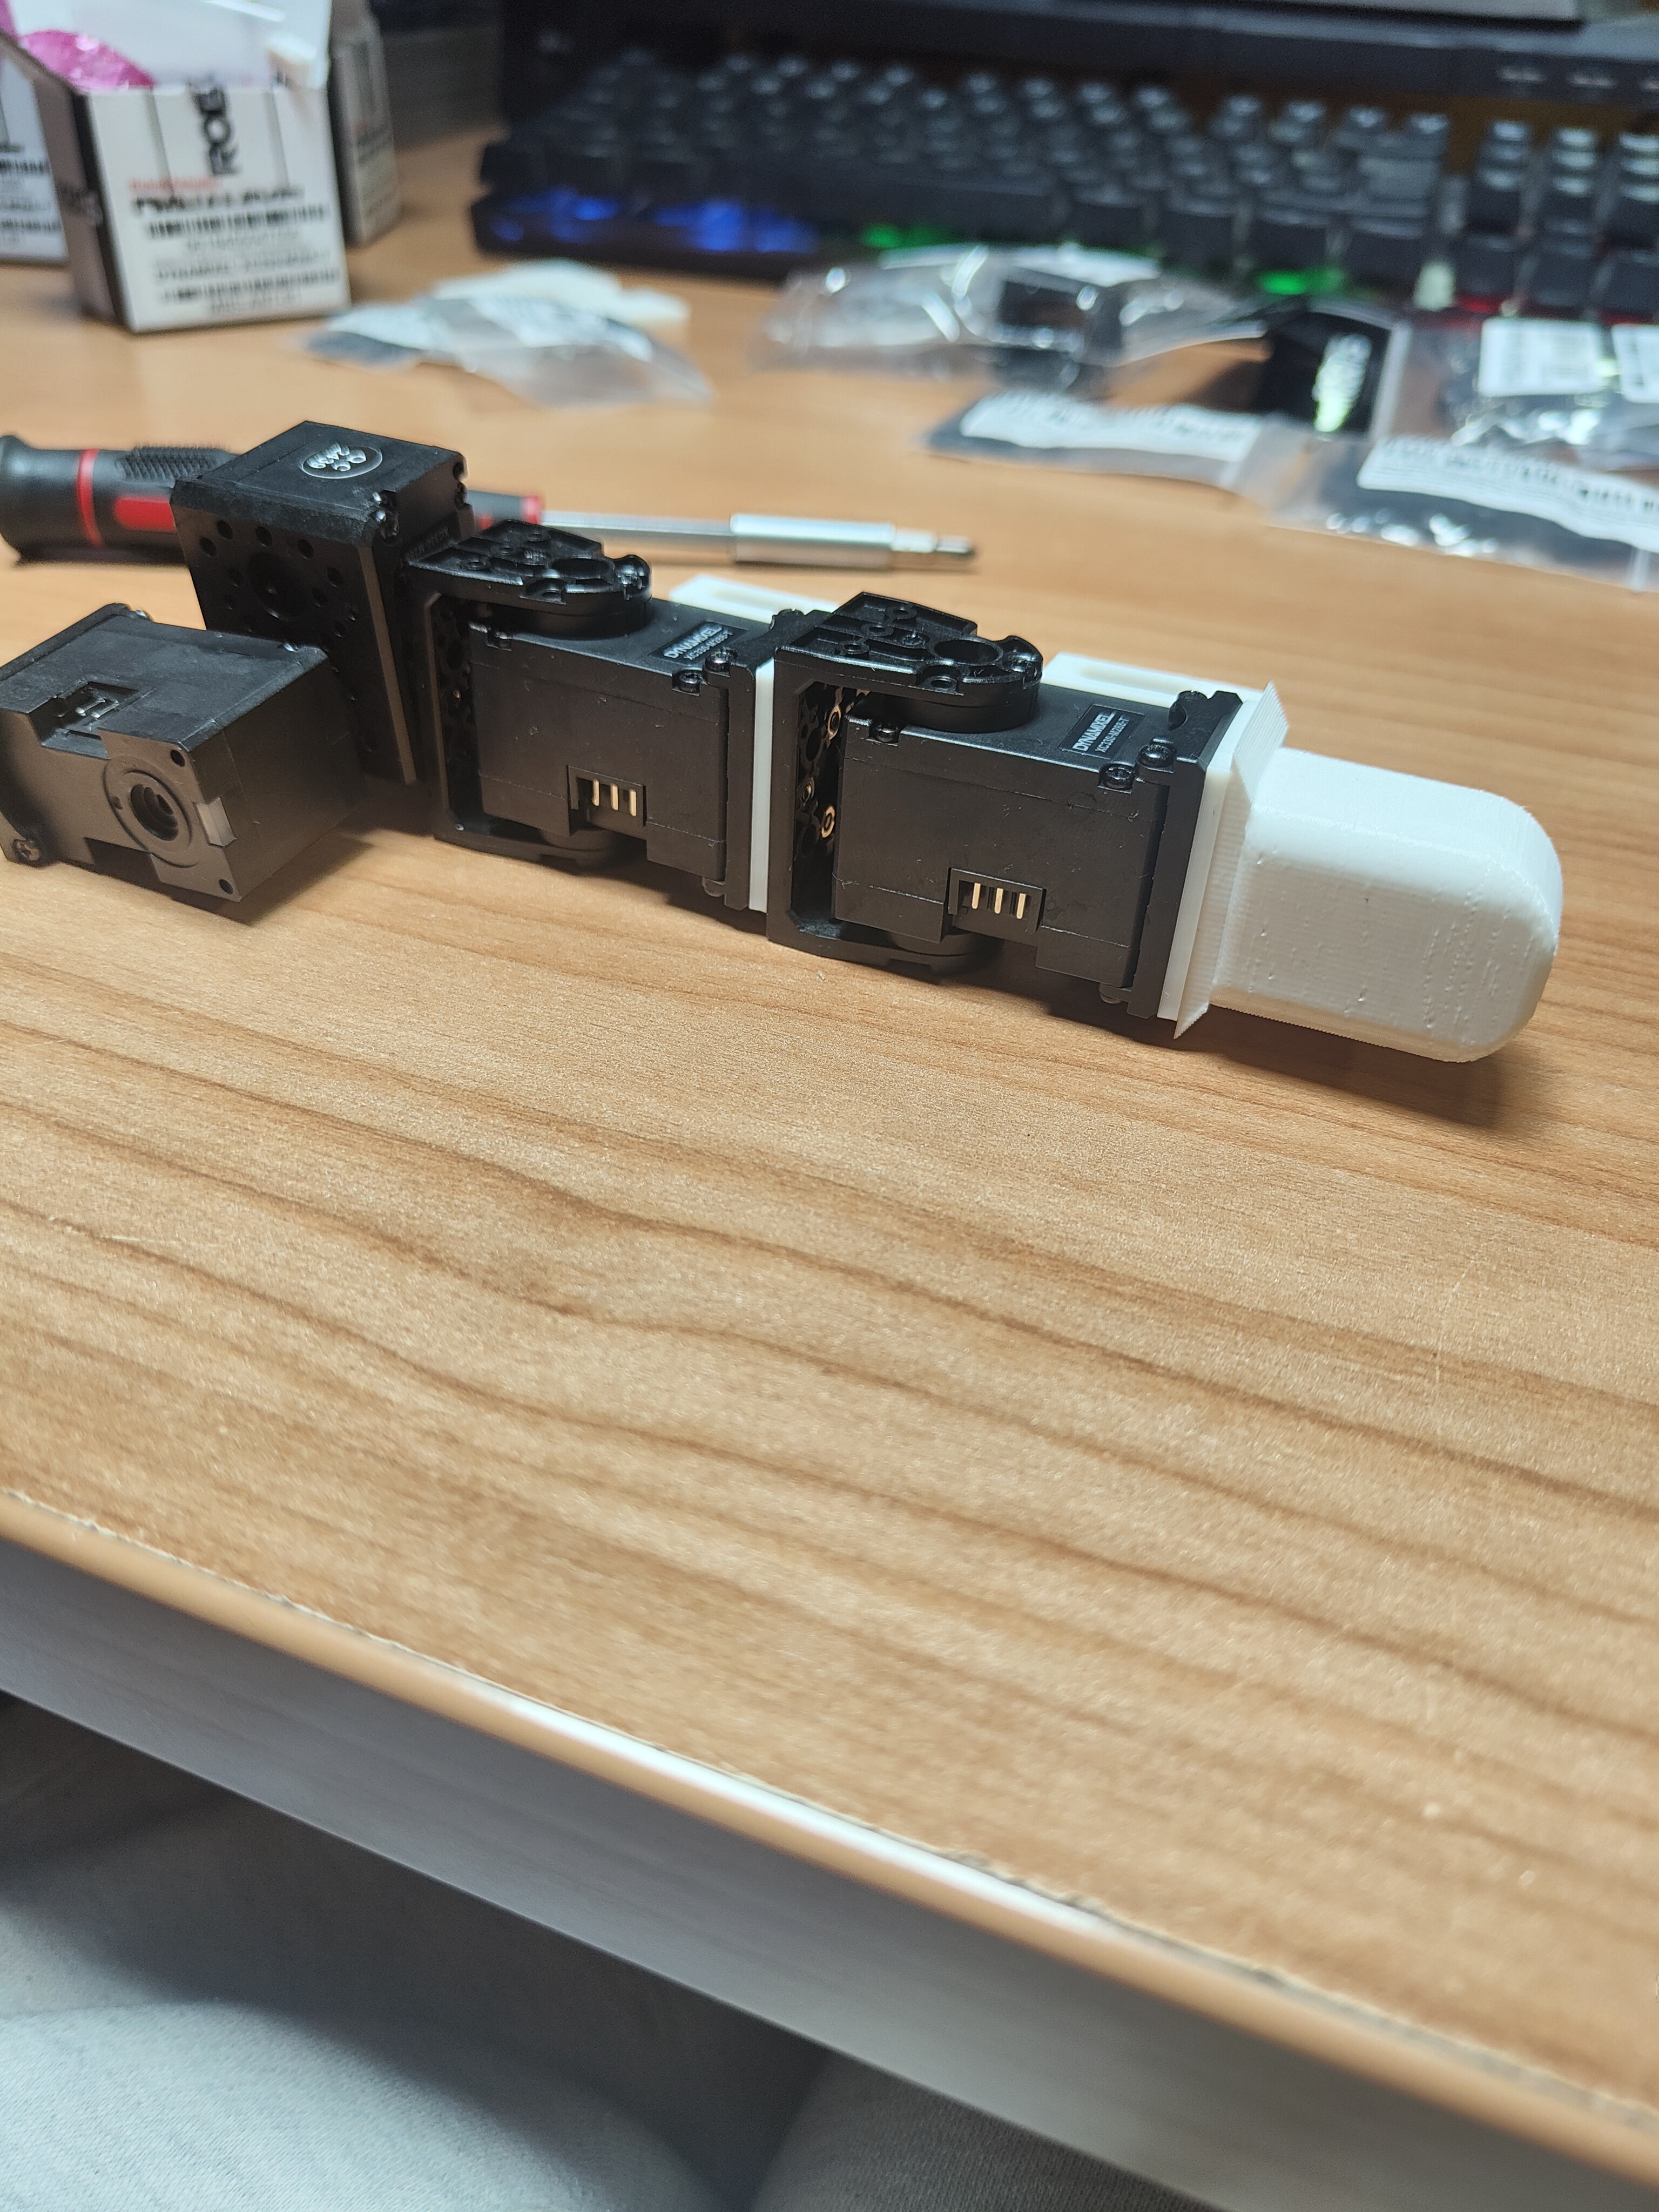
\includegraphics[width=0.25\textwidth]{figs/appendix/polegar/9.jpg} \\
\end{tabular}
\caption{Fotografias sequenciais da montagem do polegar}
\end{figure}
\label{appendix:montagem_polegar}

\subsection{Montagem dos restantes dedos}

\begin{figure}[H]
\centering
\begin{tabular}{ccc}
  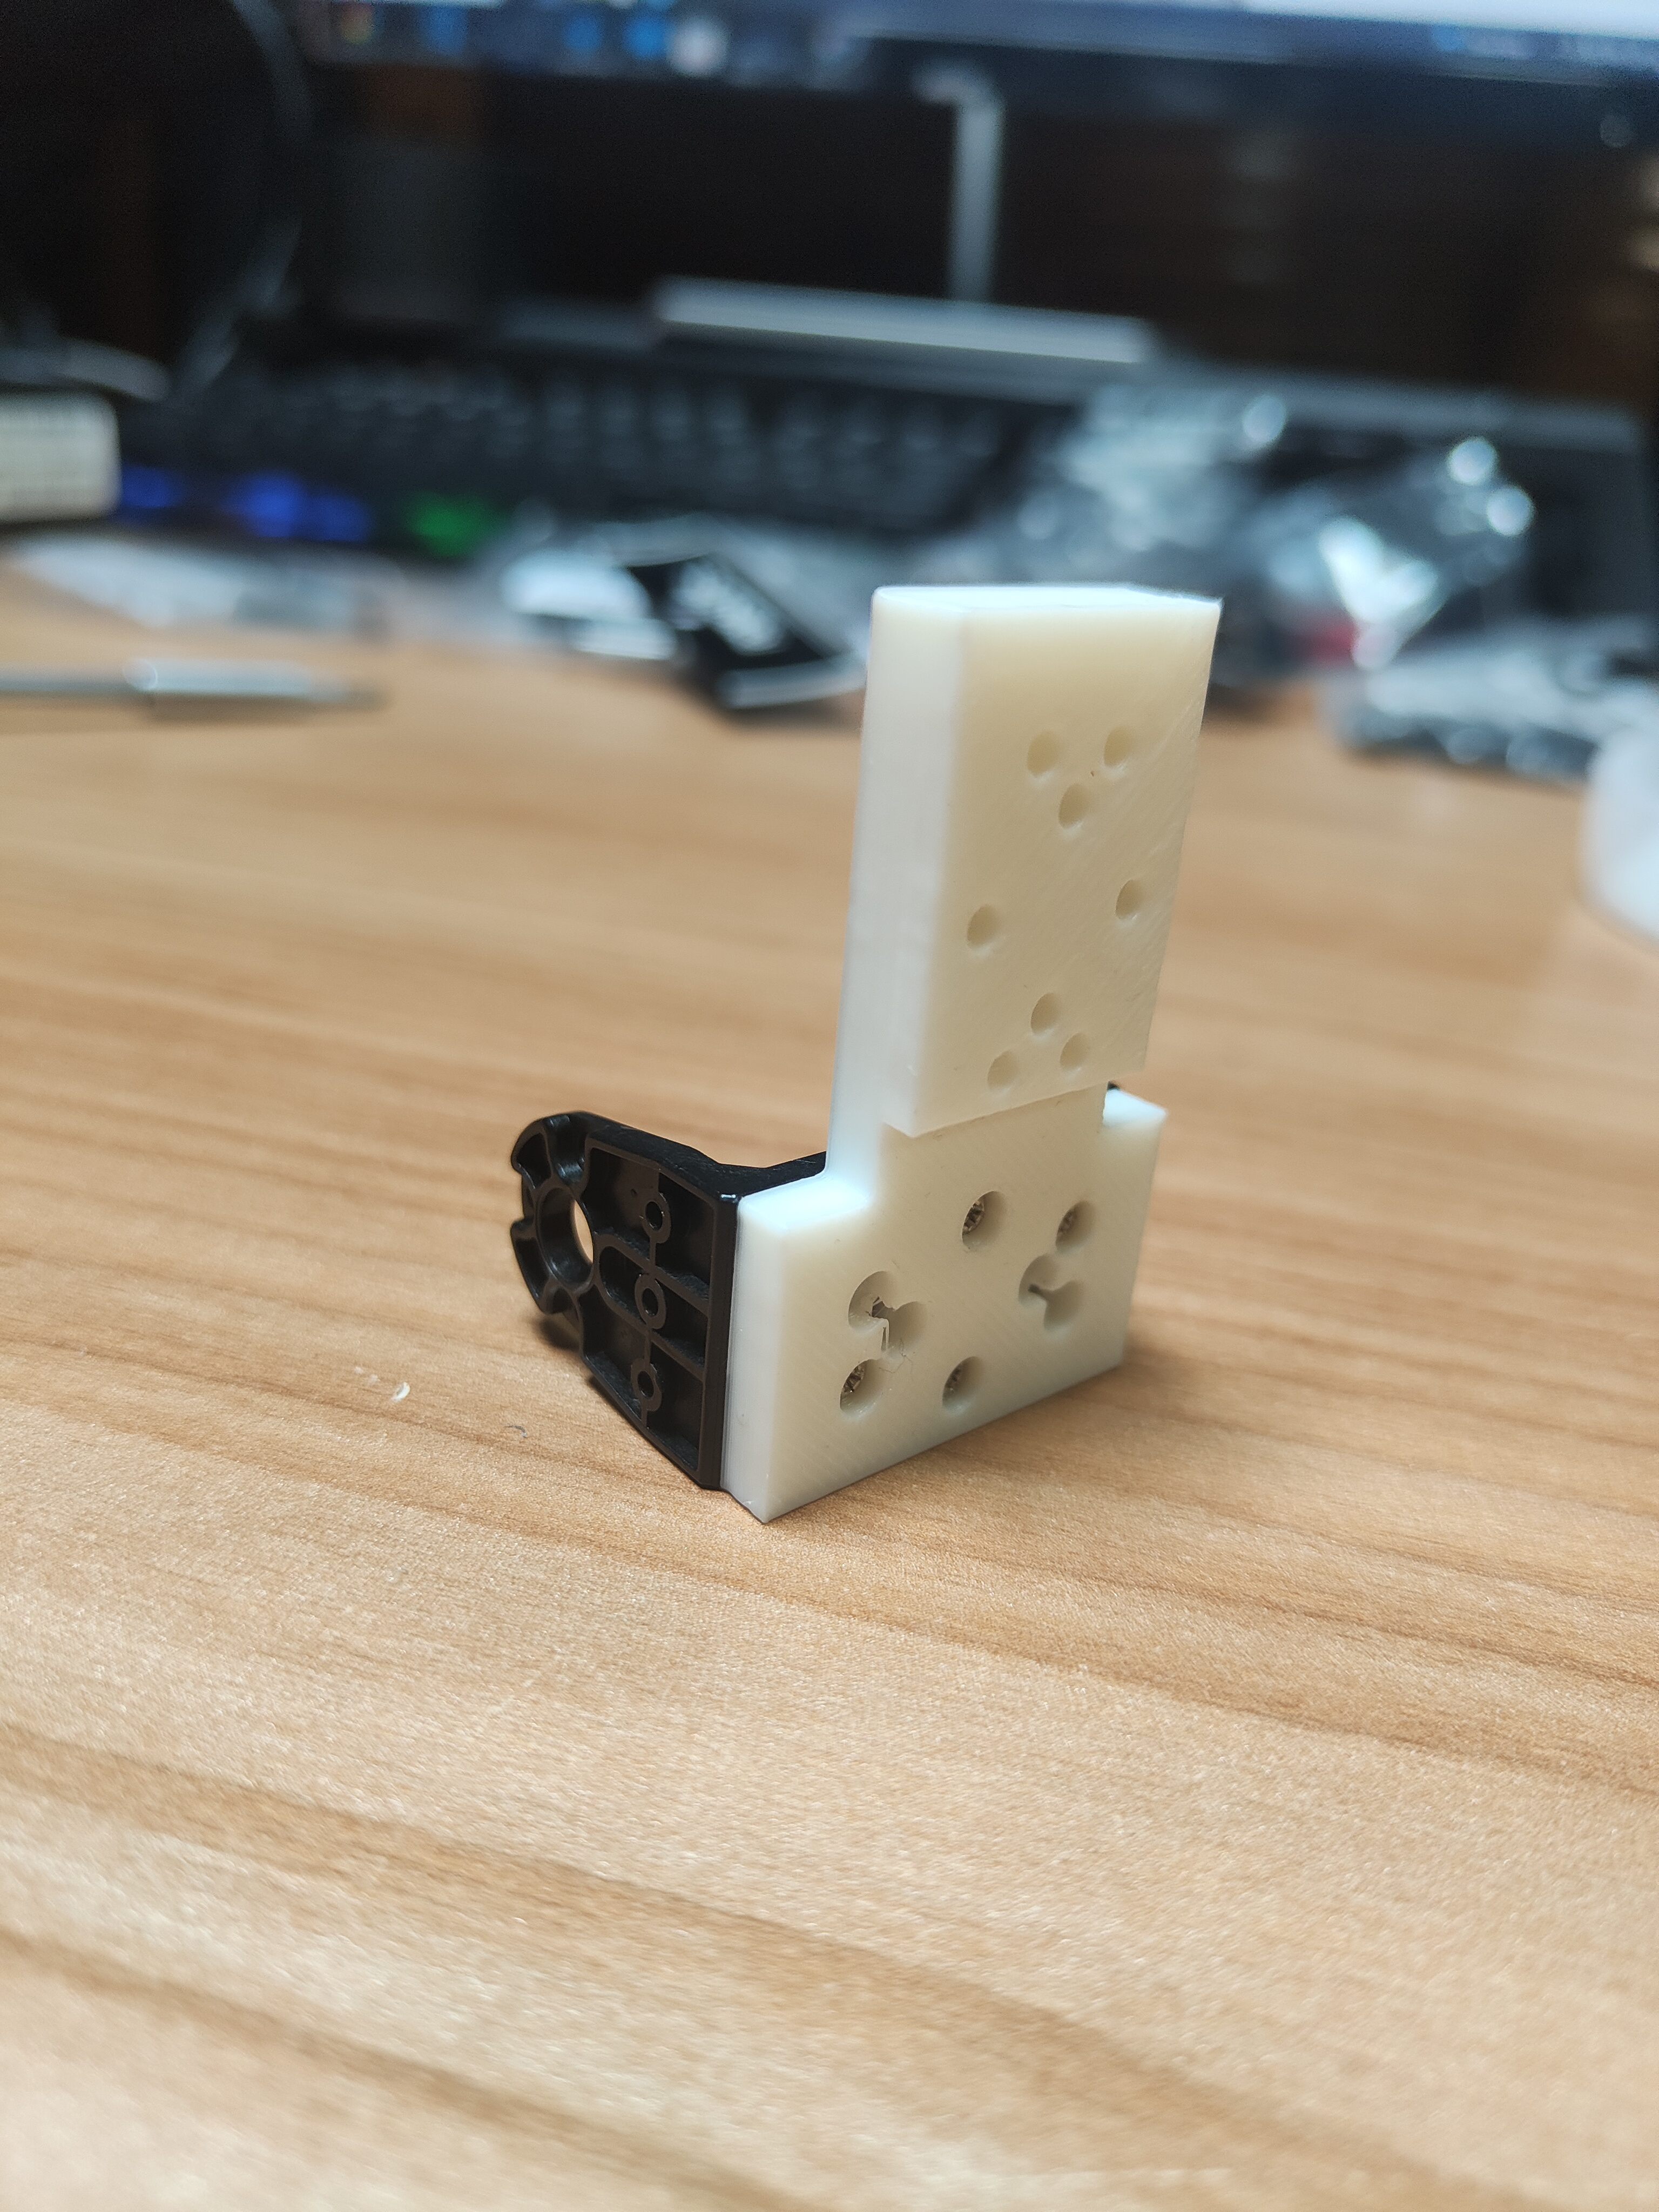
\includegraphics[width=0.25\textwidth]{figs/appendix/dedo/1.jpg} &
  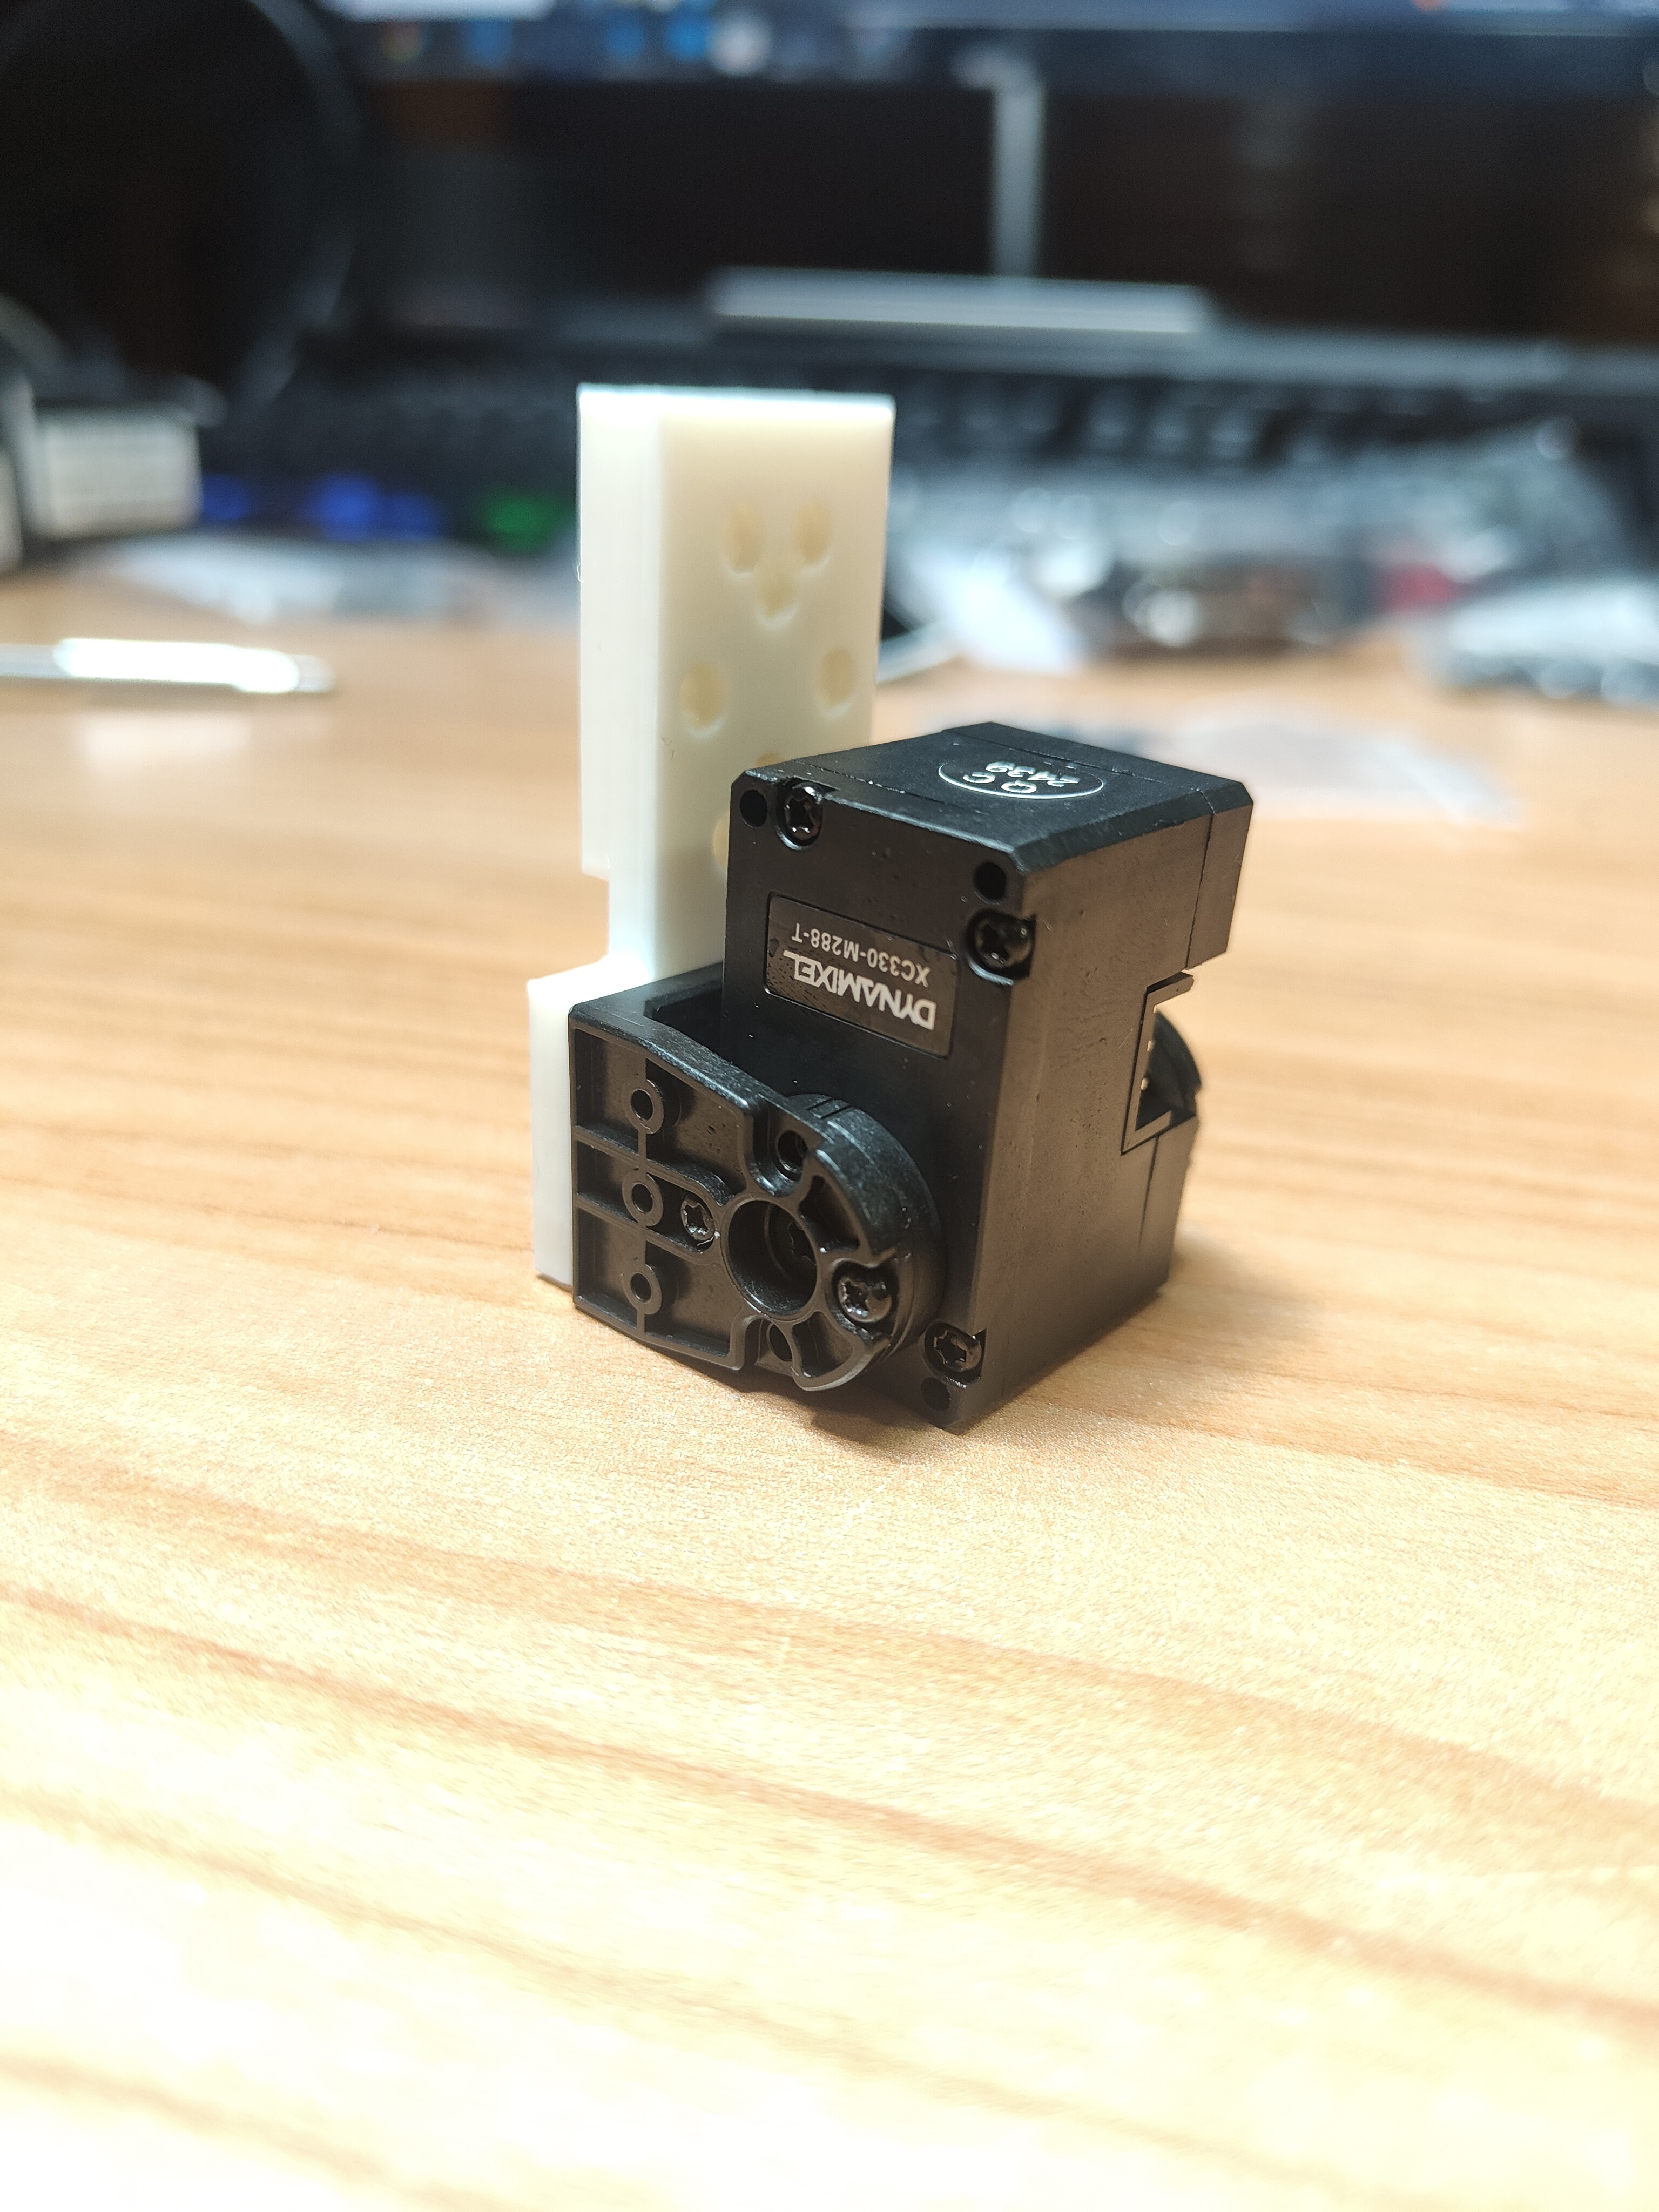
\includegraphics[width=0.25\textwidth]{figs/appendix/dedo/2.jpg} &
  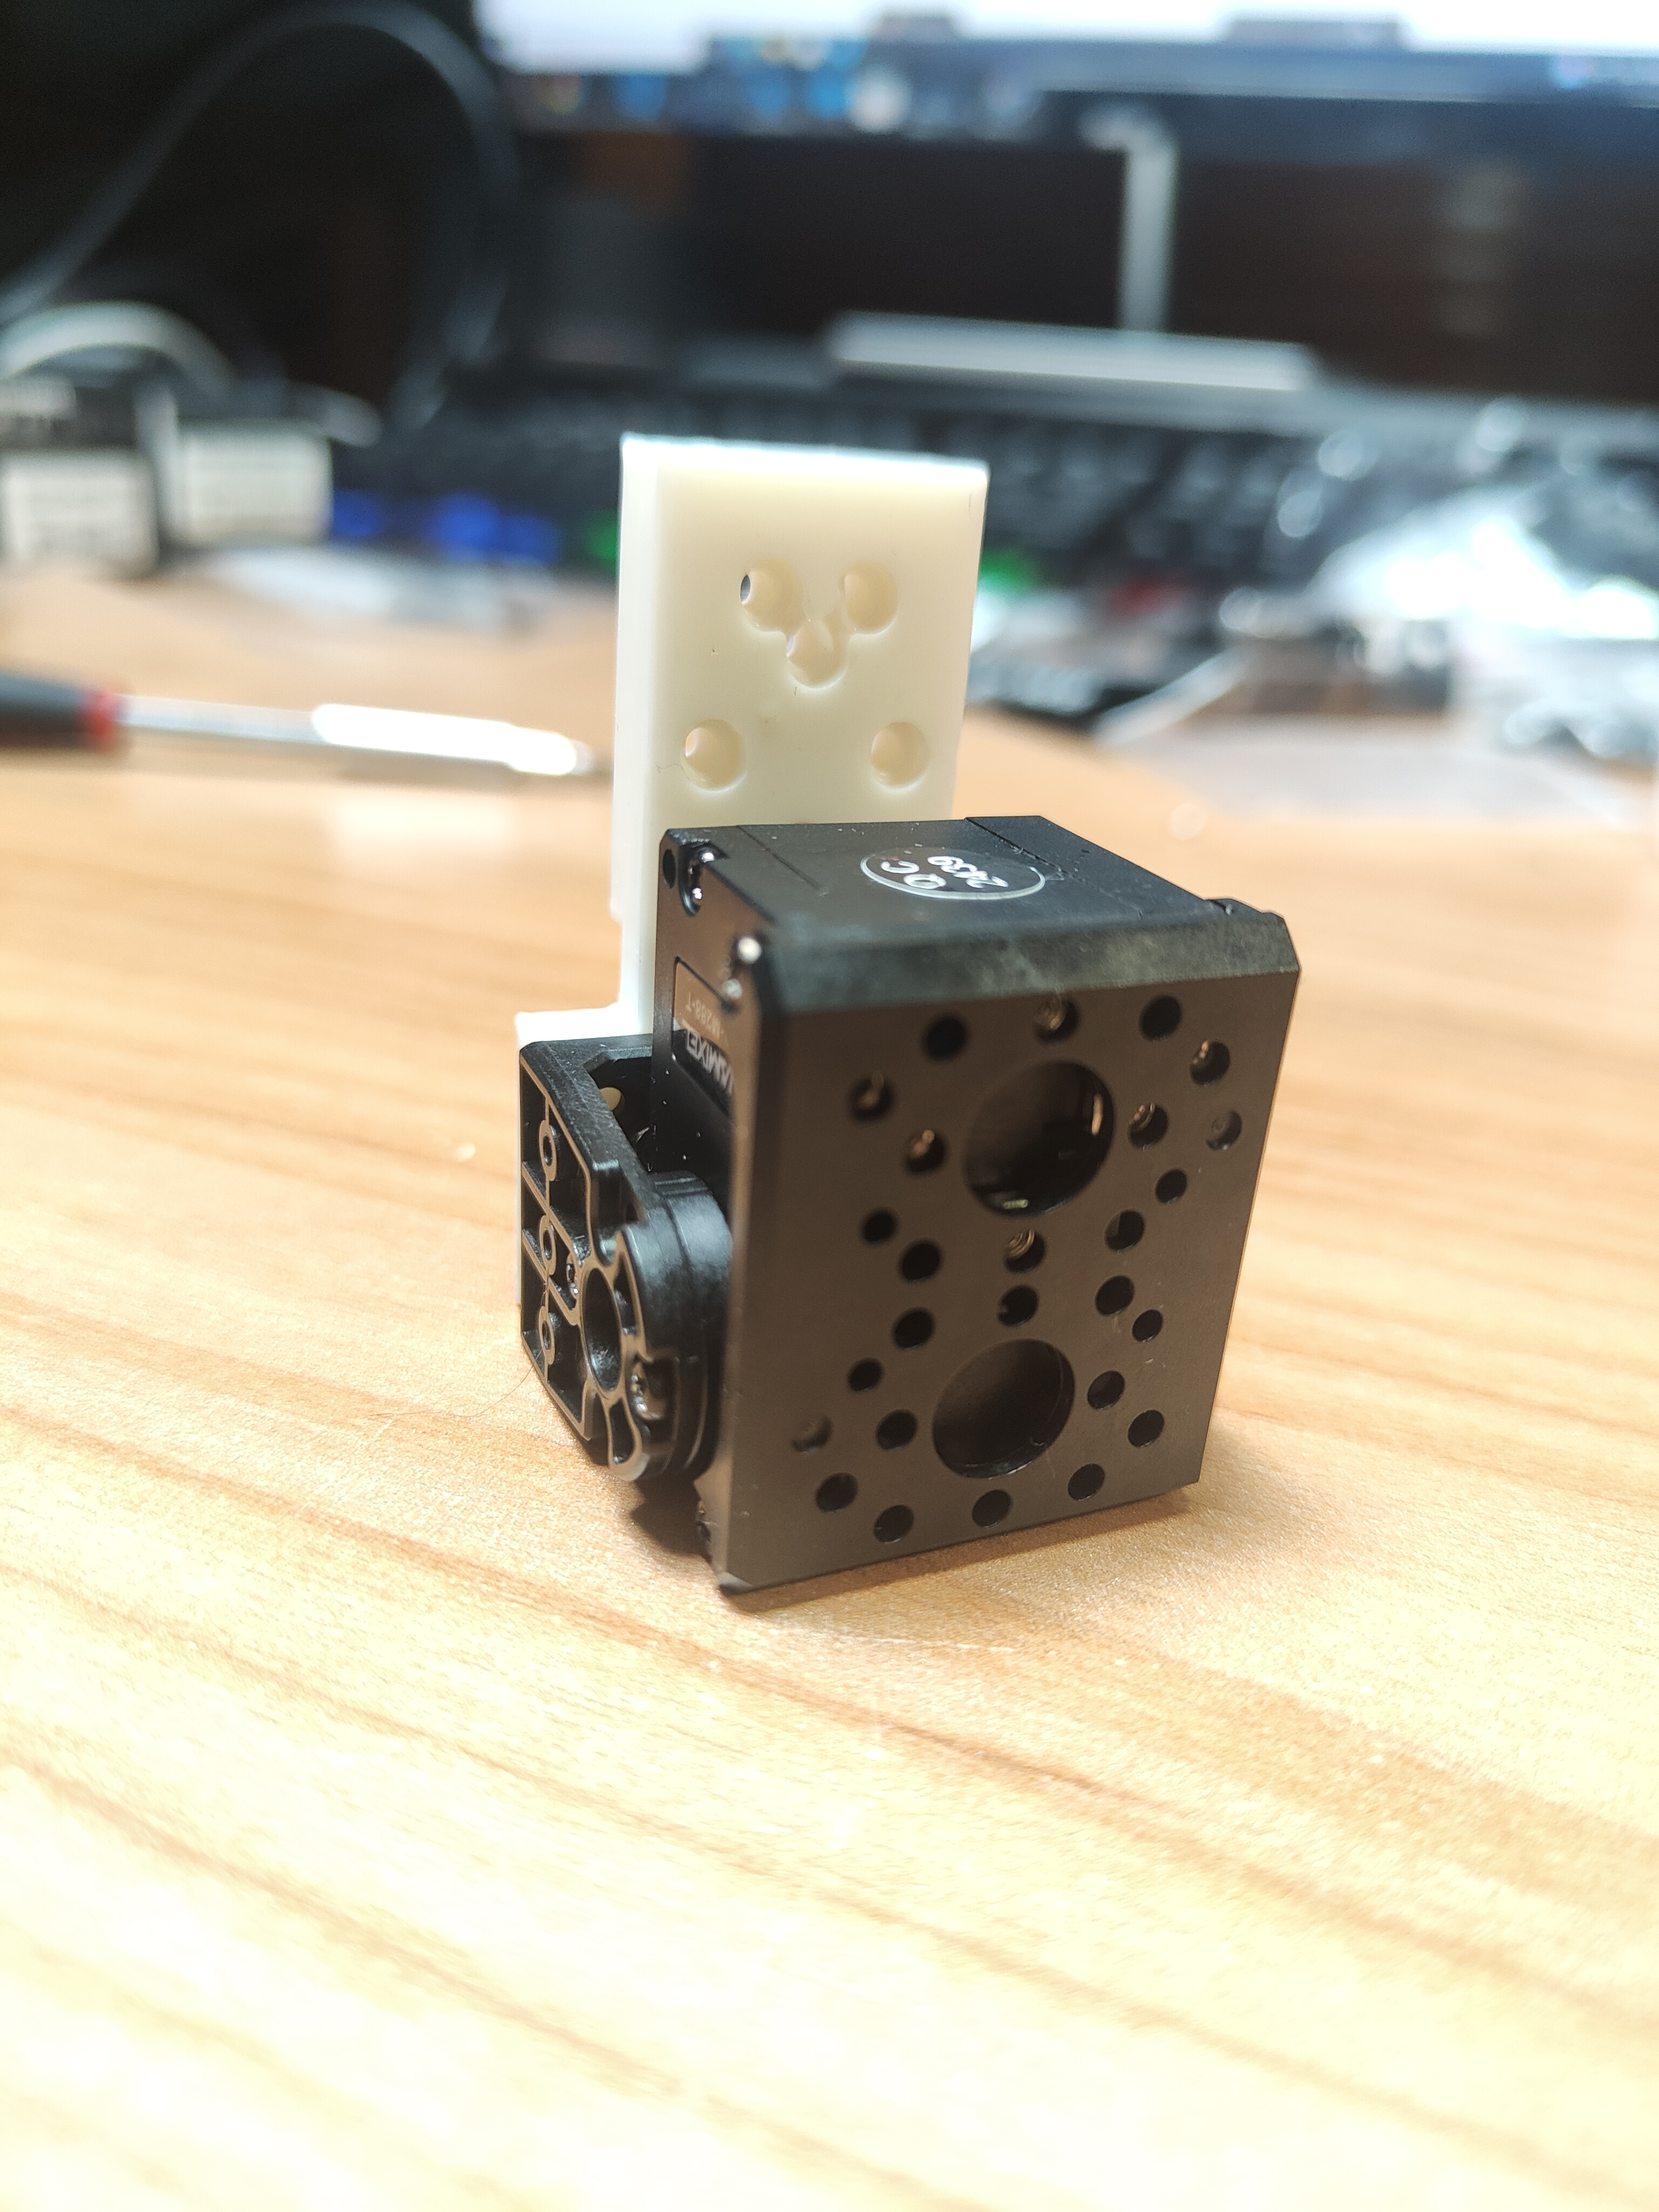
\includegraphics[width=0.25\textwidth]{figs/appendix/dedo/3.jpg} \\
  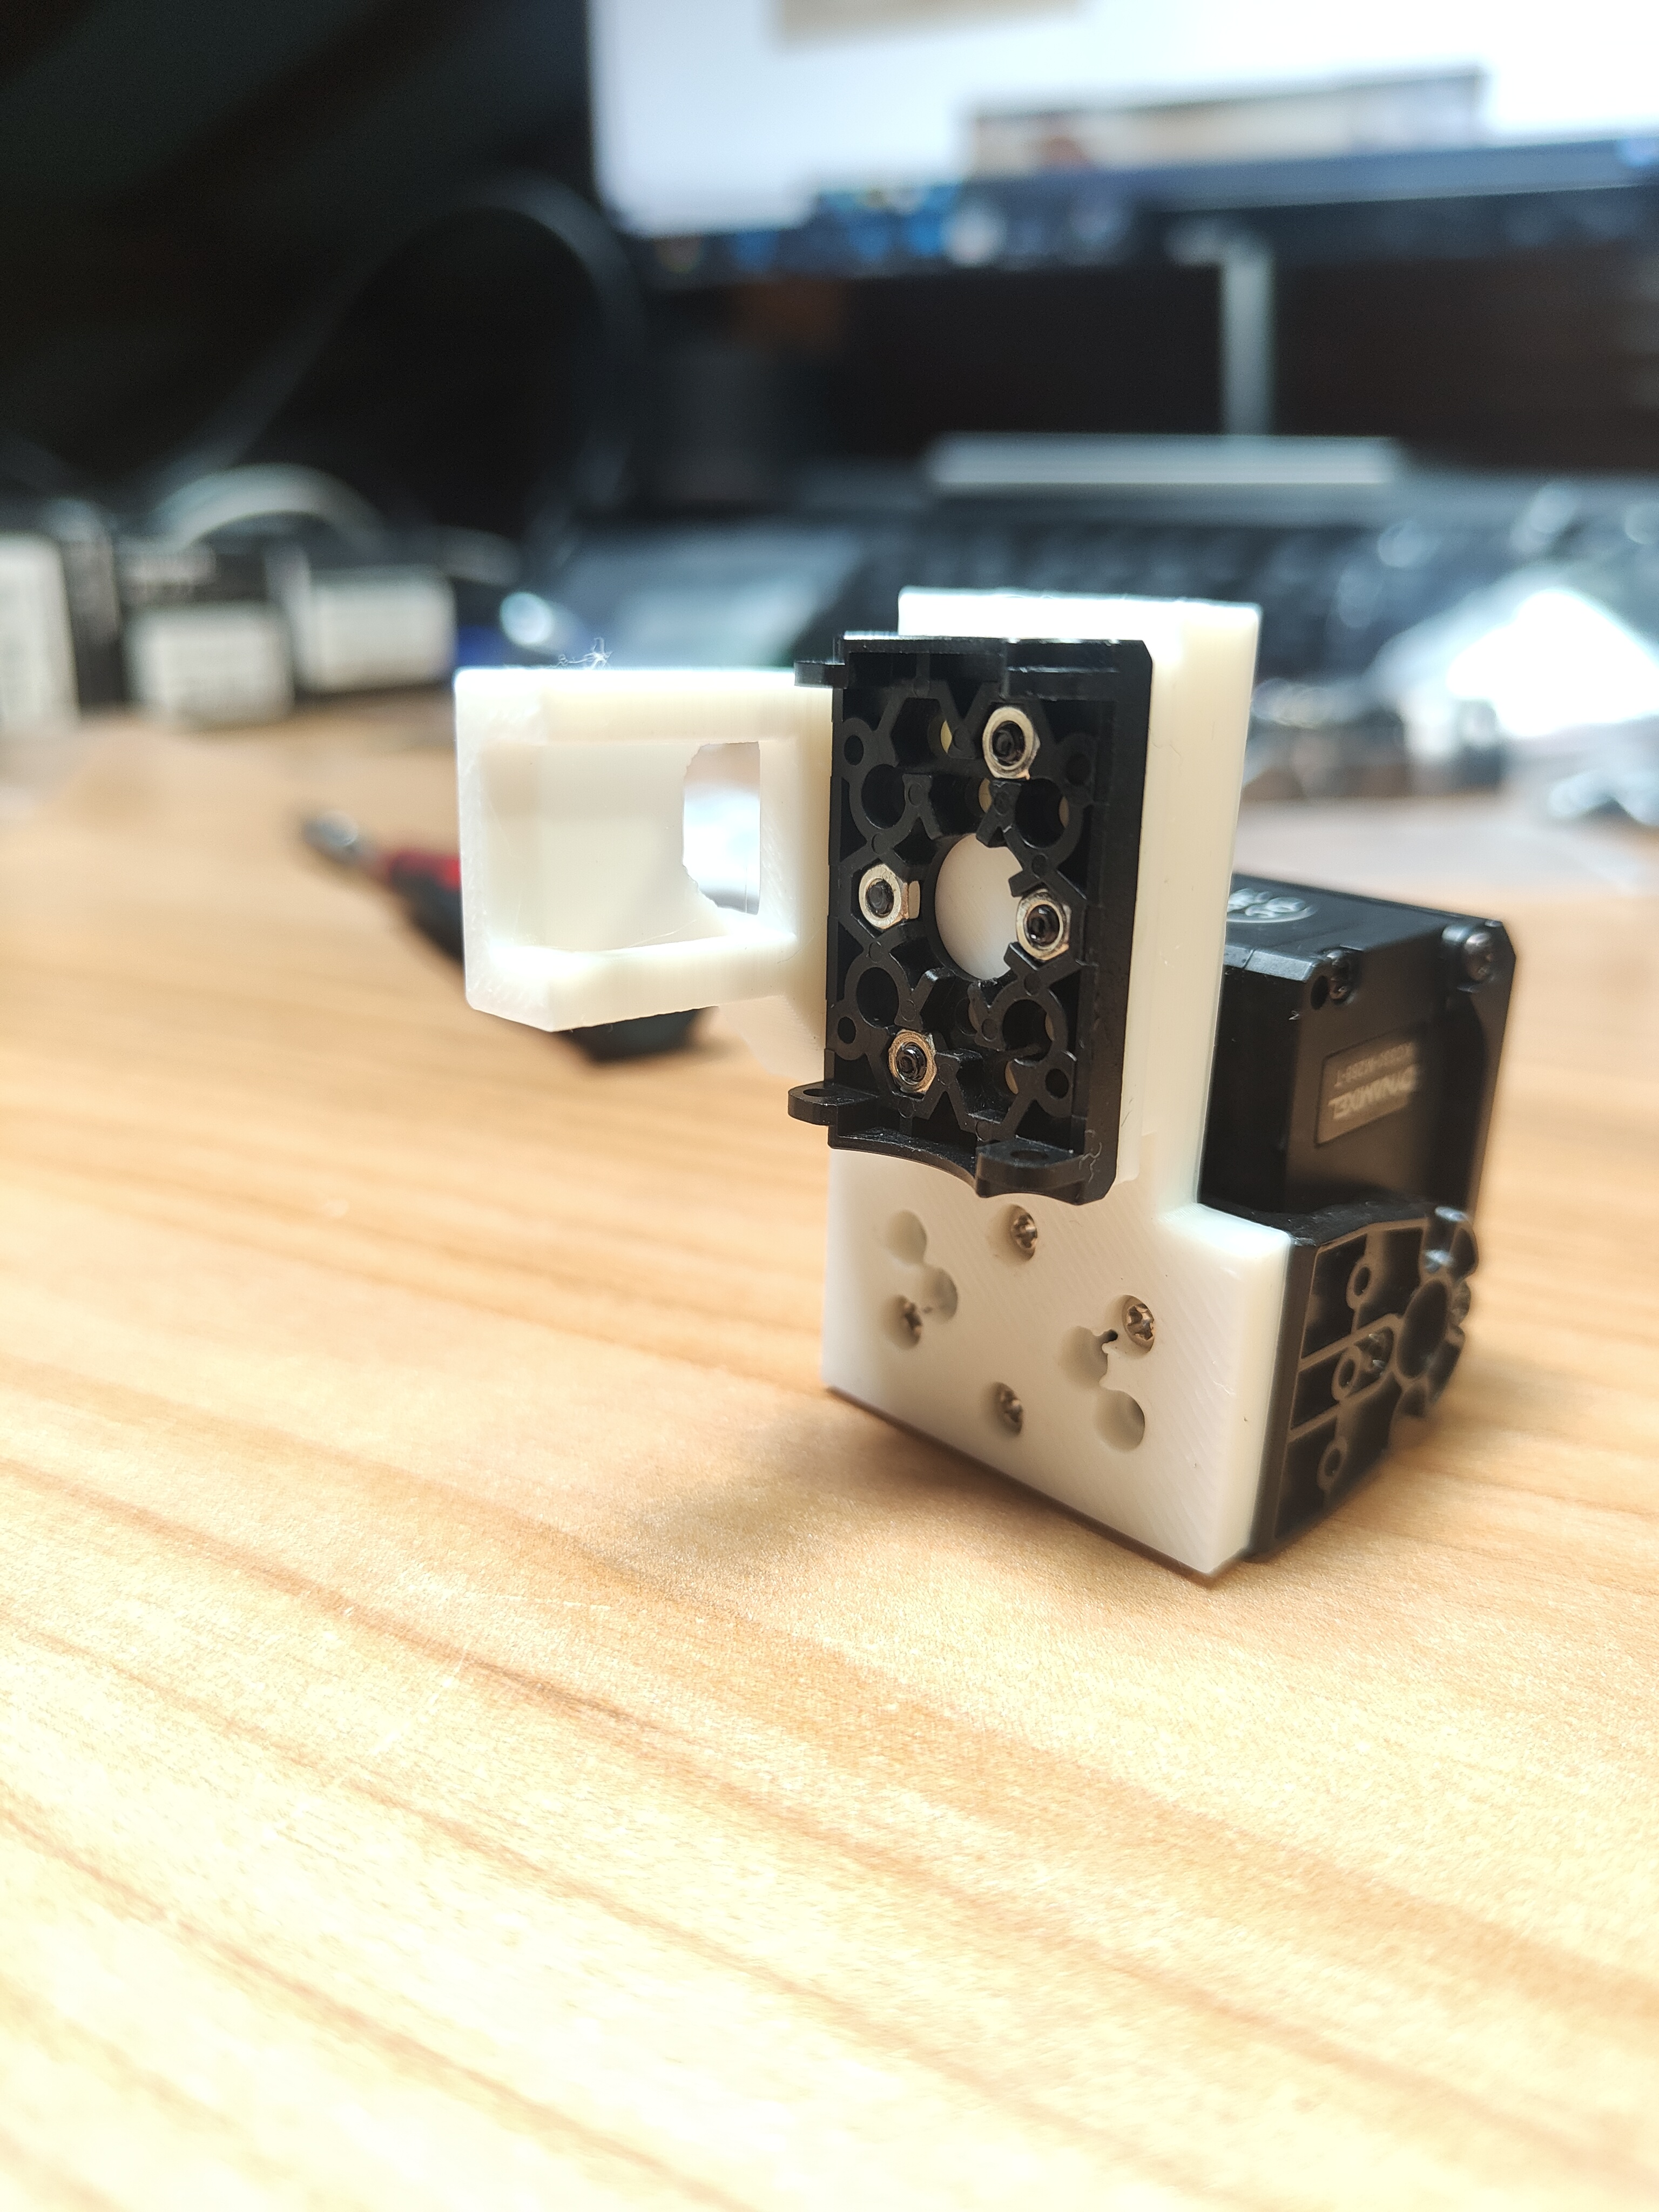
\includegraphics[width=0.25\textwidth]{figs/appendix/dedo/4.jpg} &
  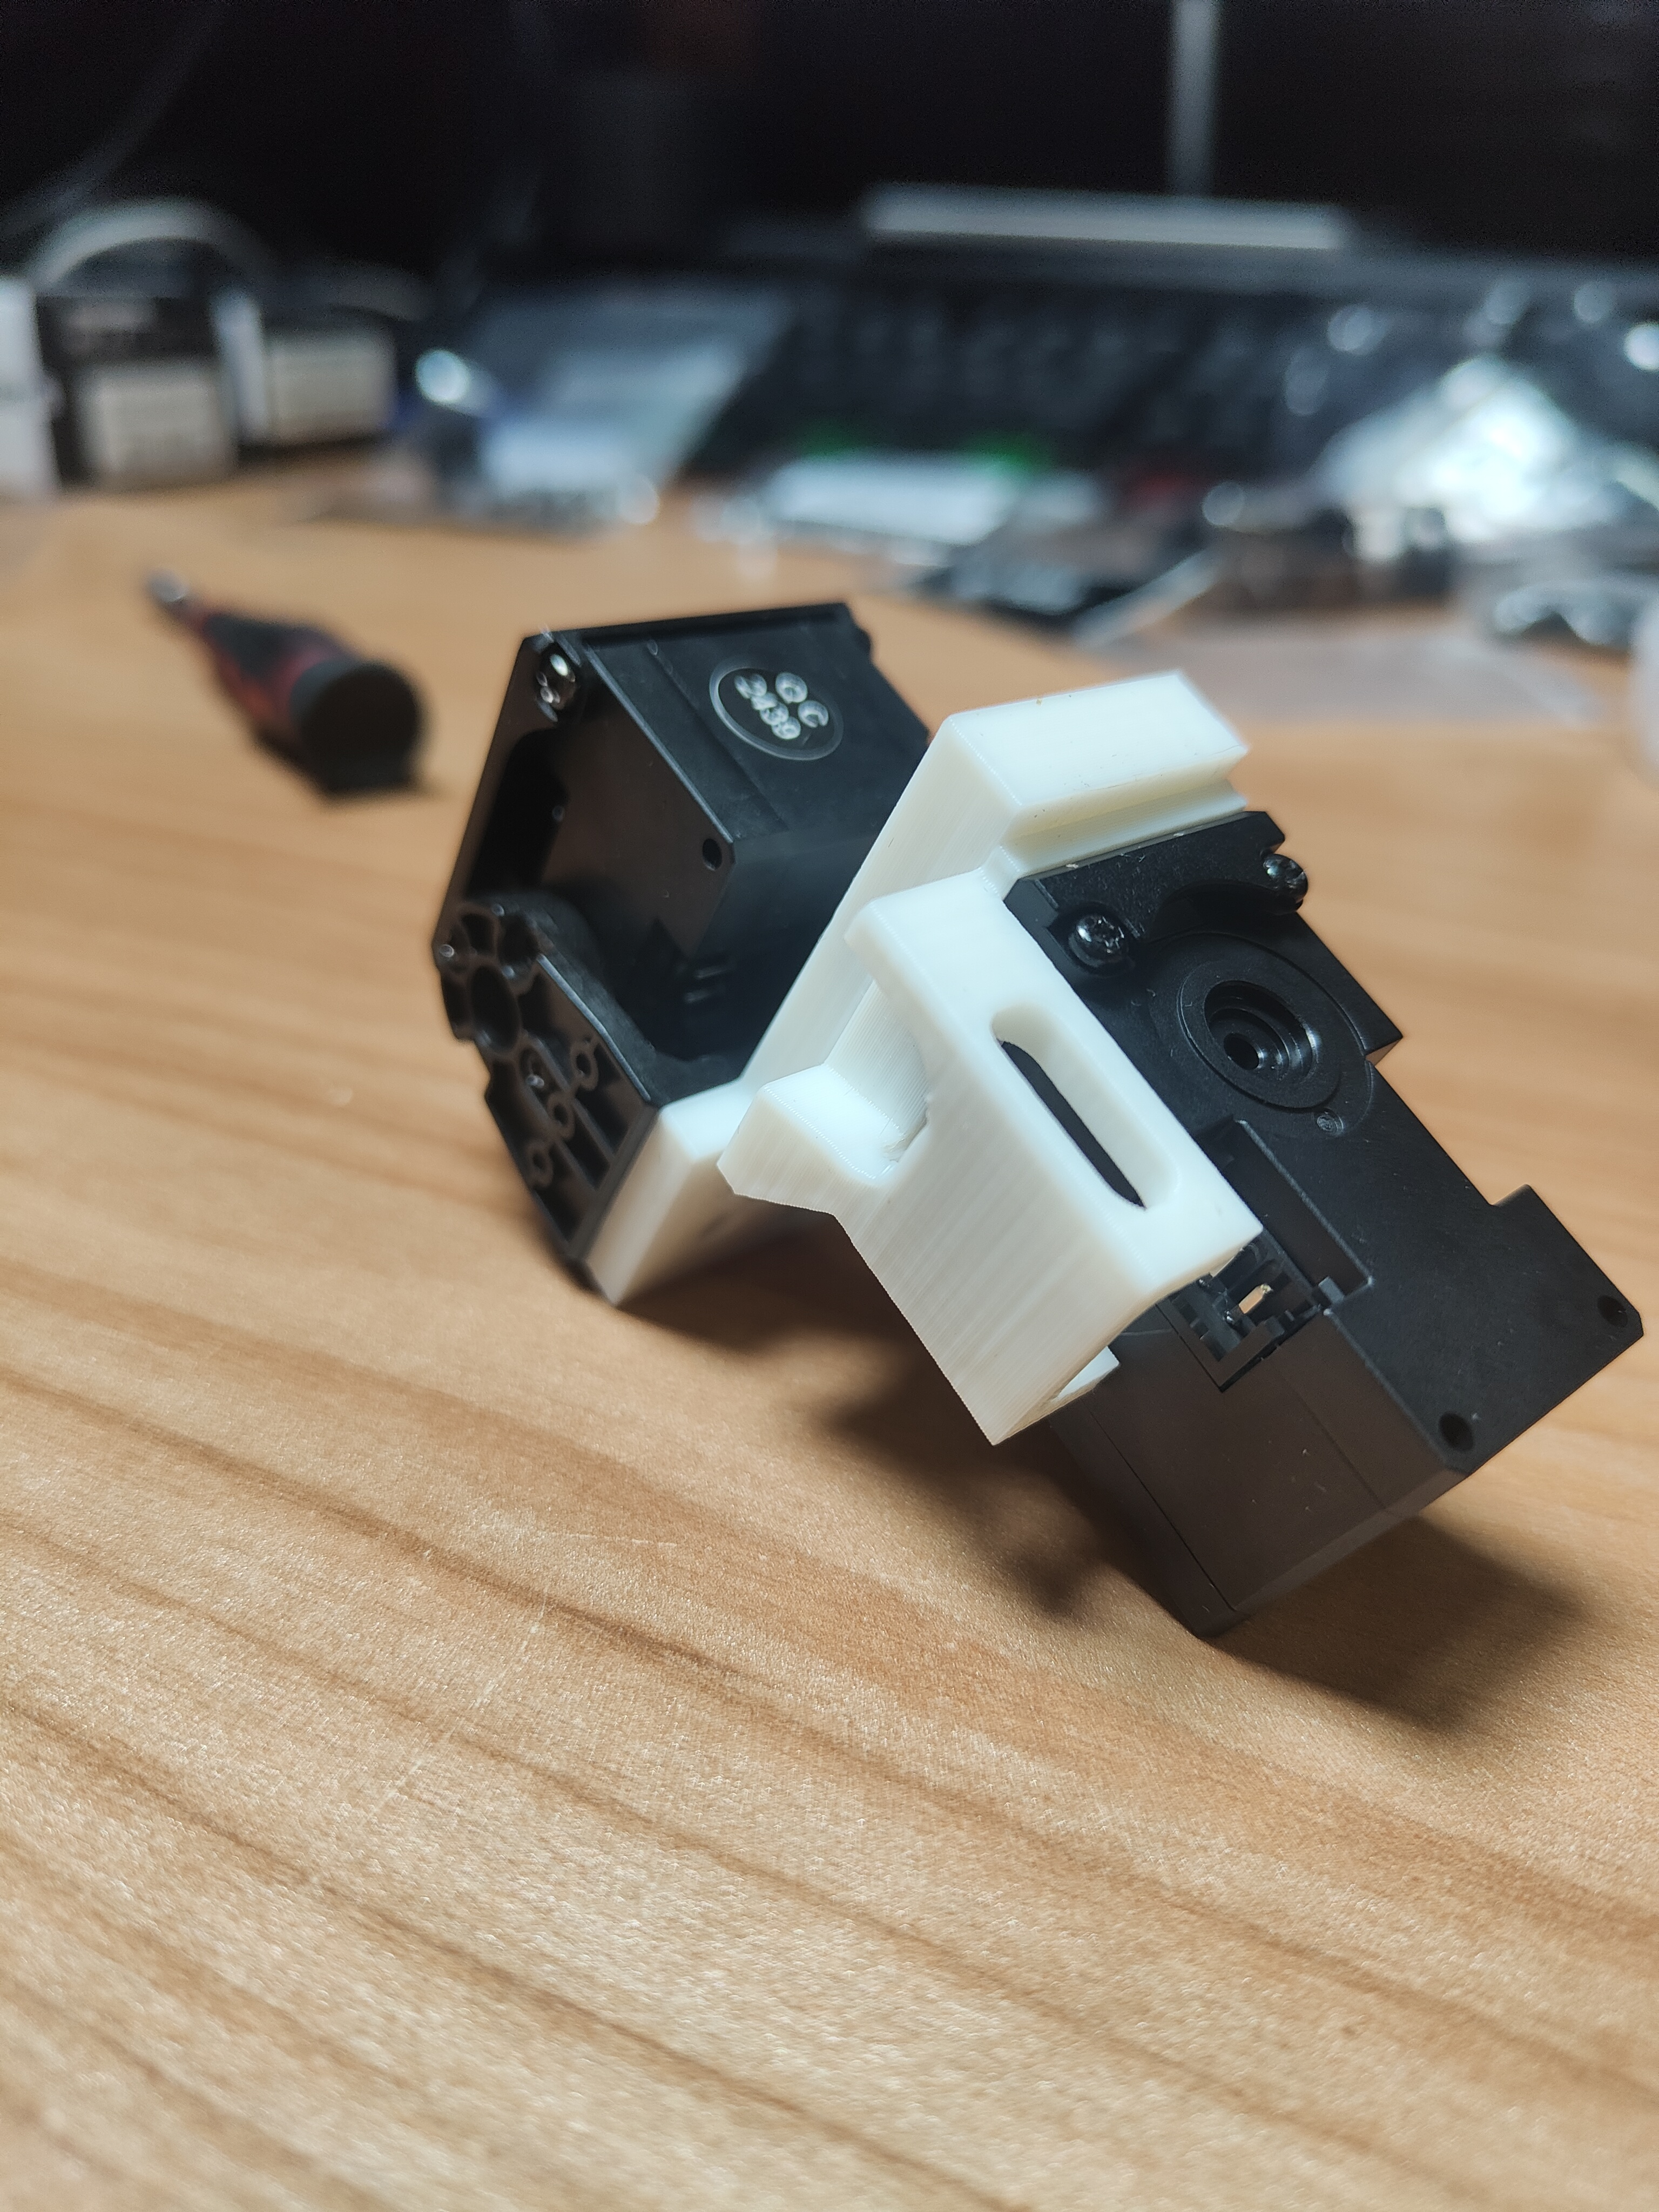
\includegraphics[width=0.25\textwidth]{figs/appendix/dedo/5.jpg} &
  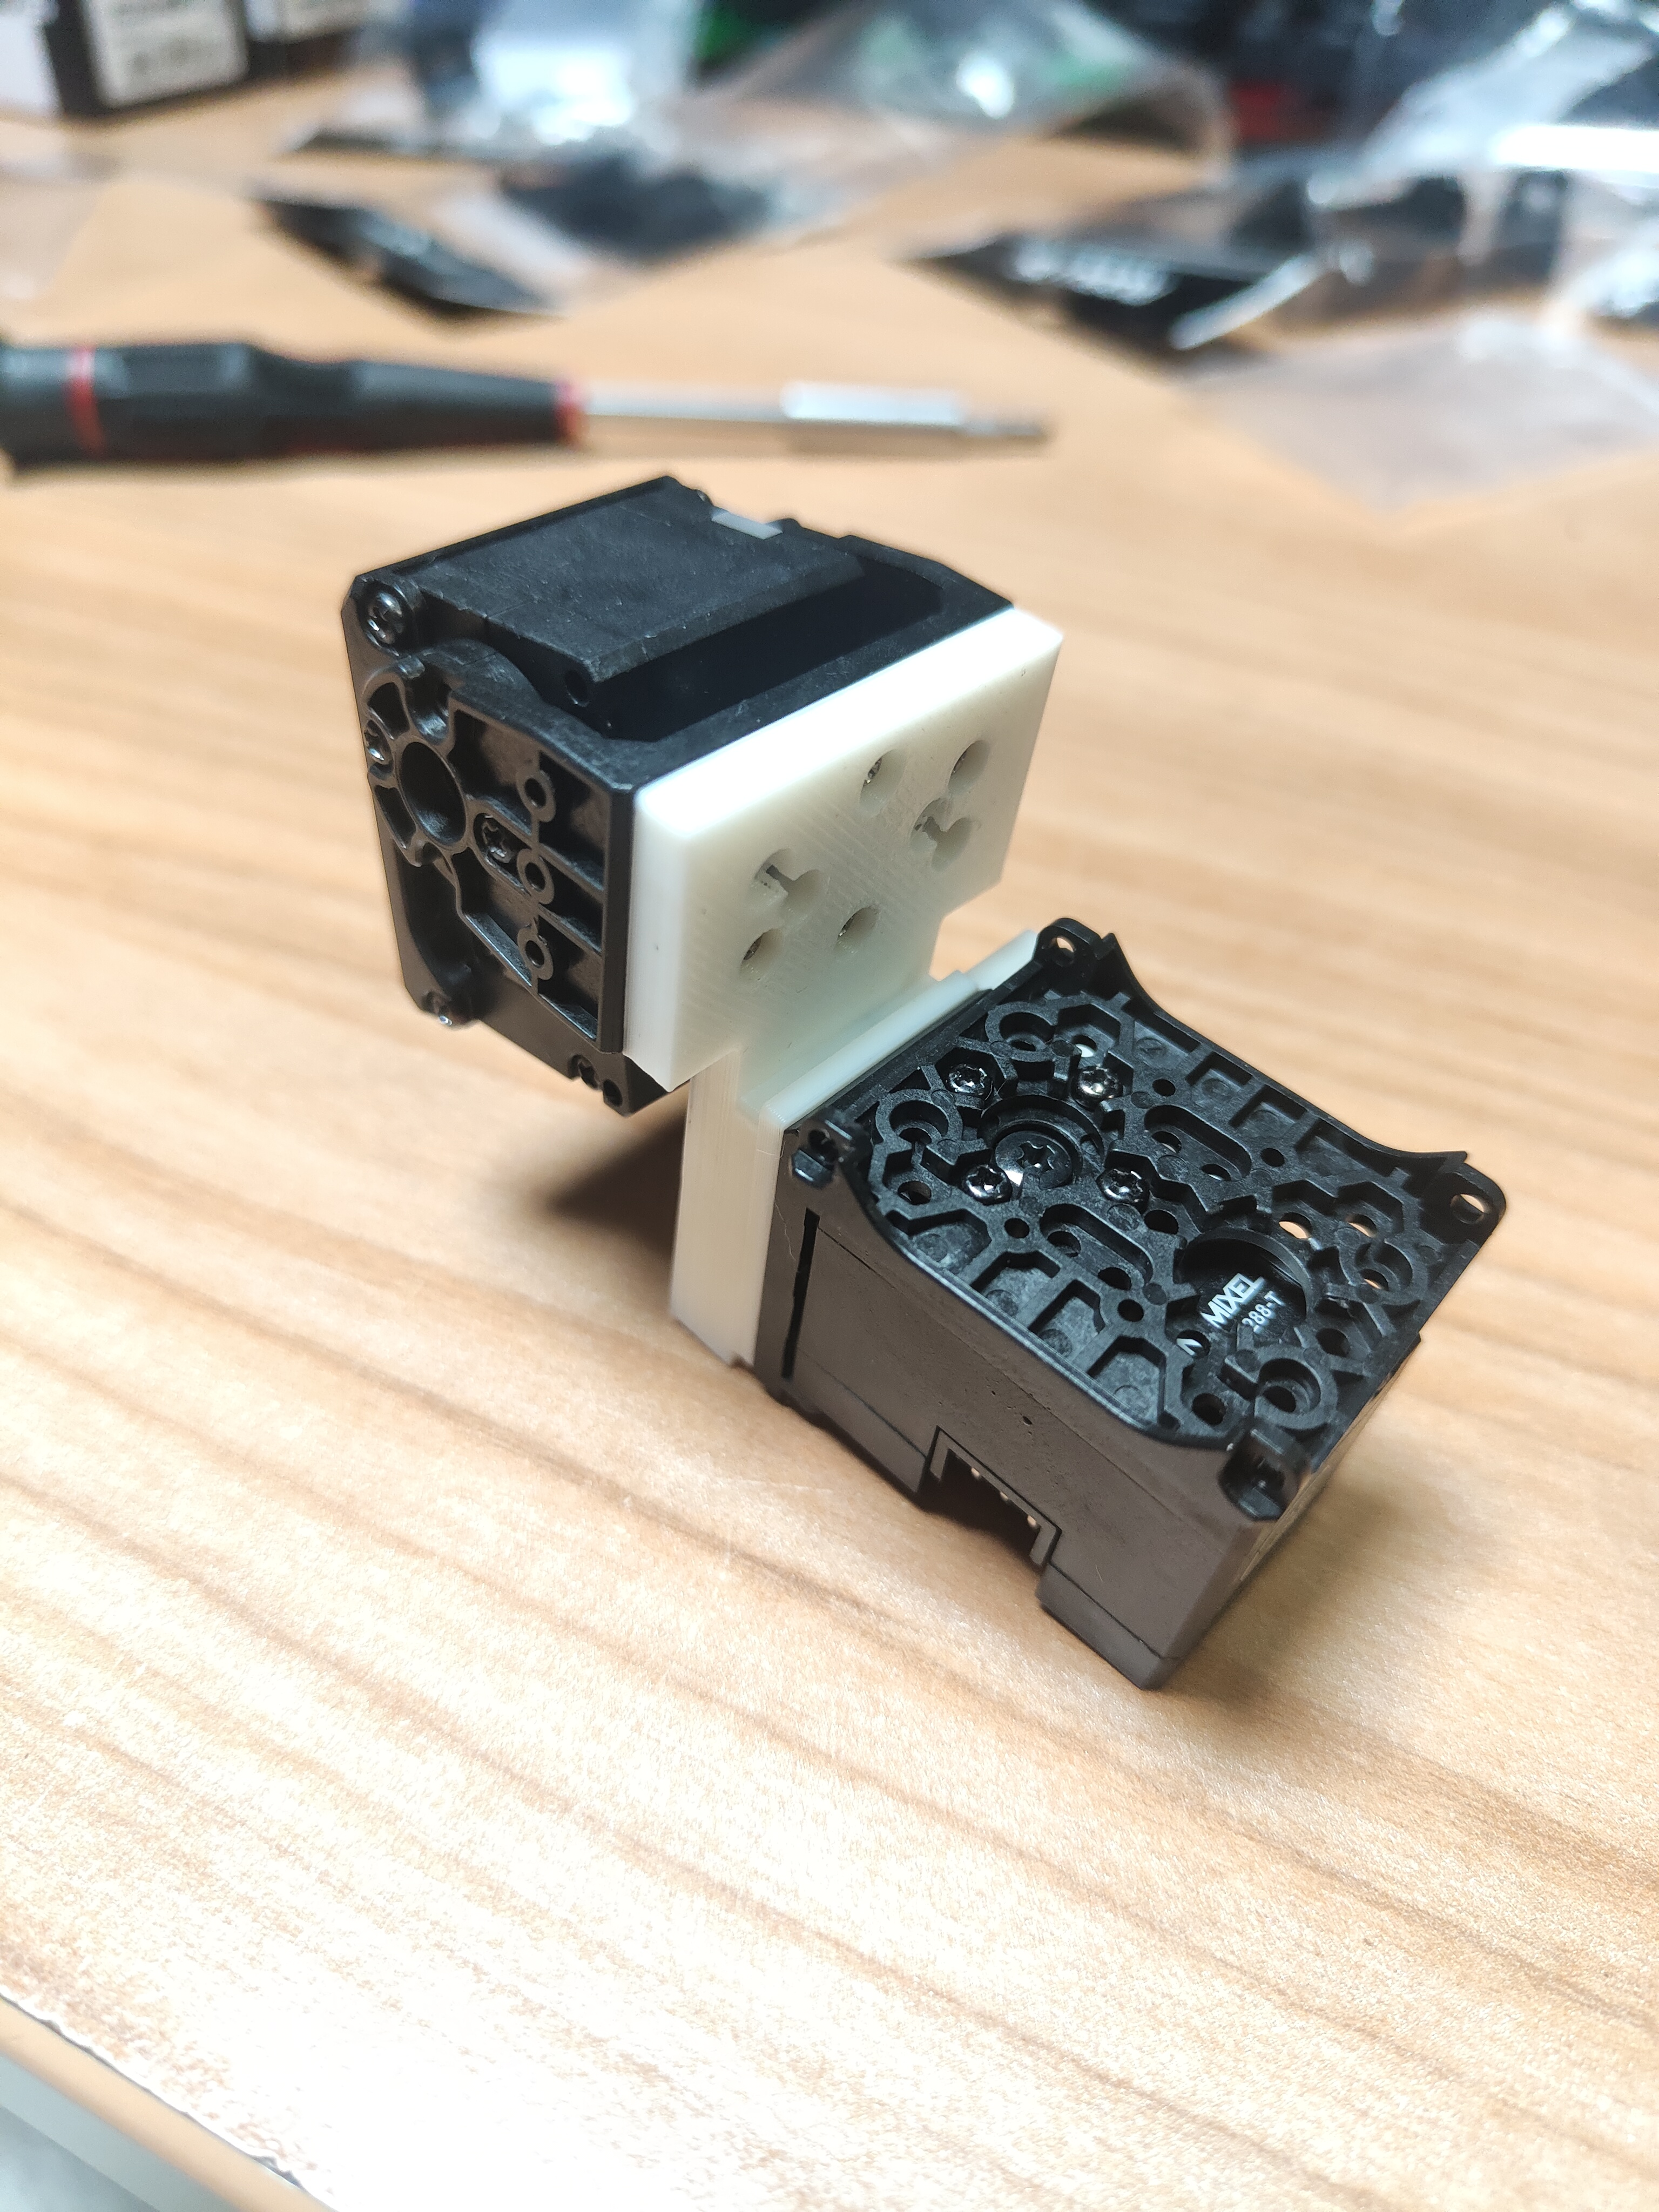
\includegraphics[width=0.25\textwidth]{figs/appendix/dedo/6.jpg} \\
  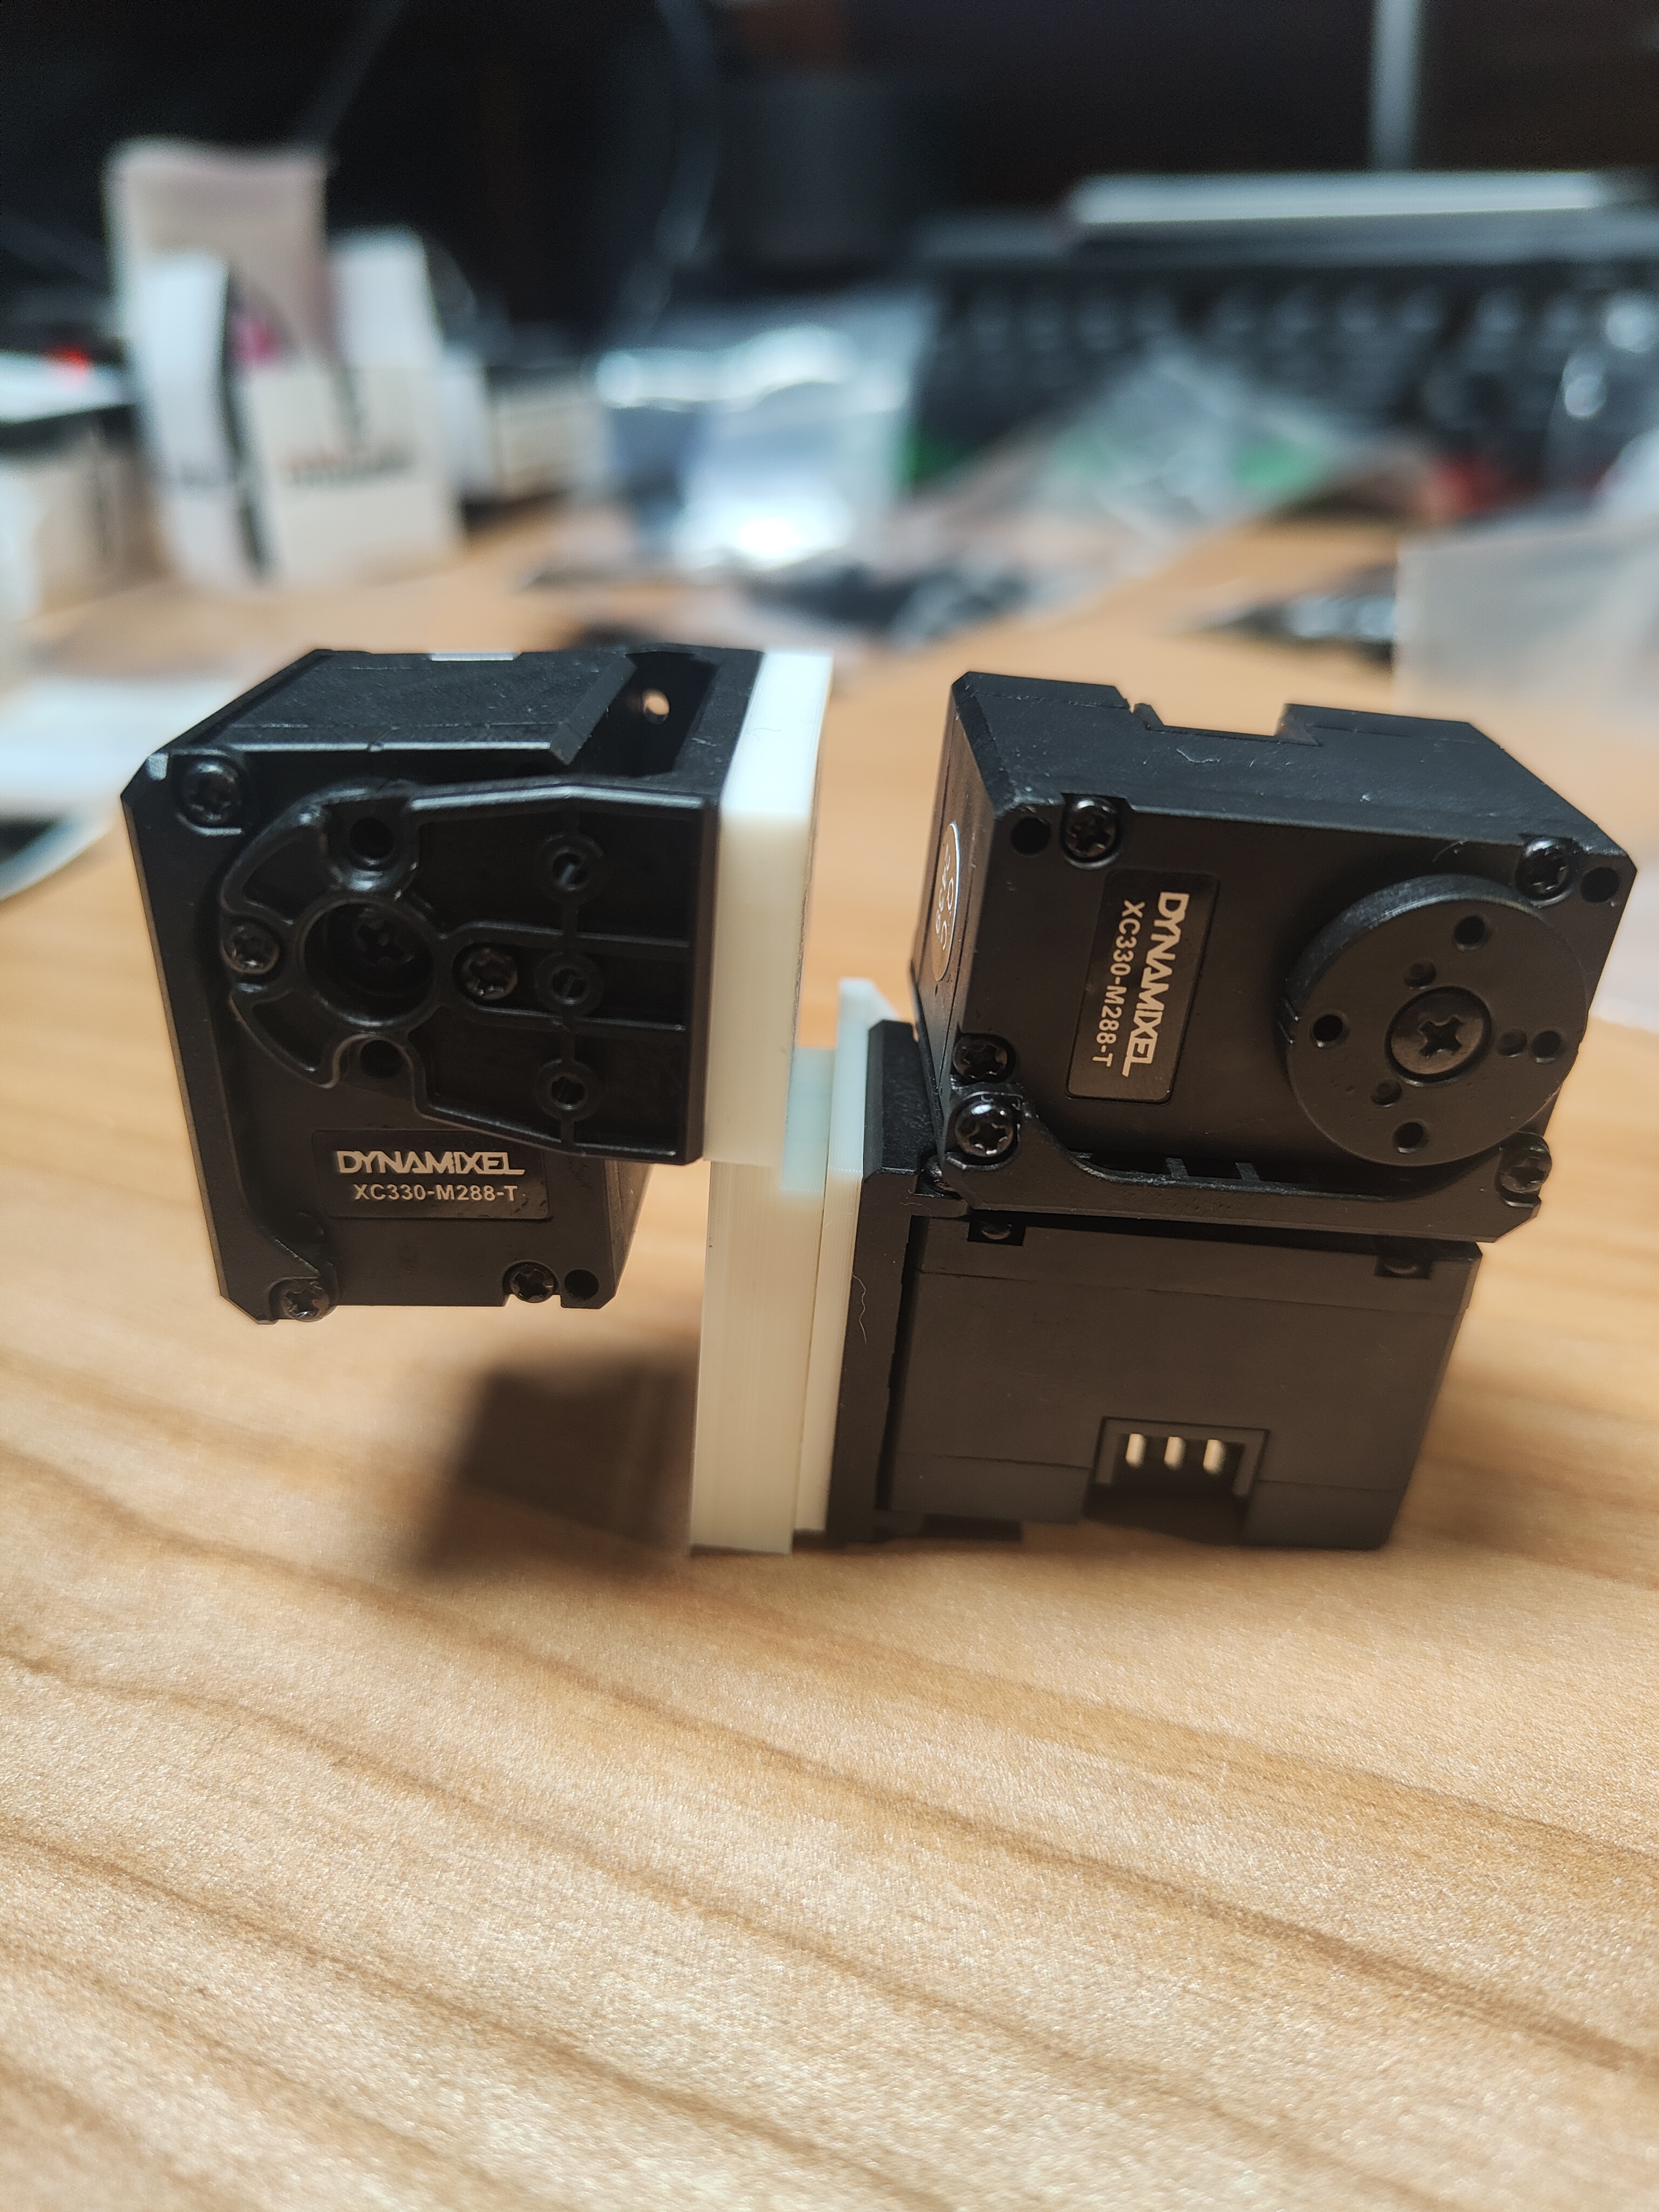
\includegraphics[width=0.25\textwidth]{figs/appendix/dedo/7.jpg} &
  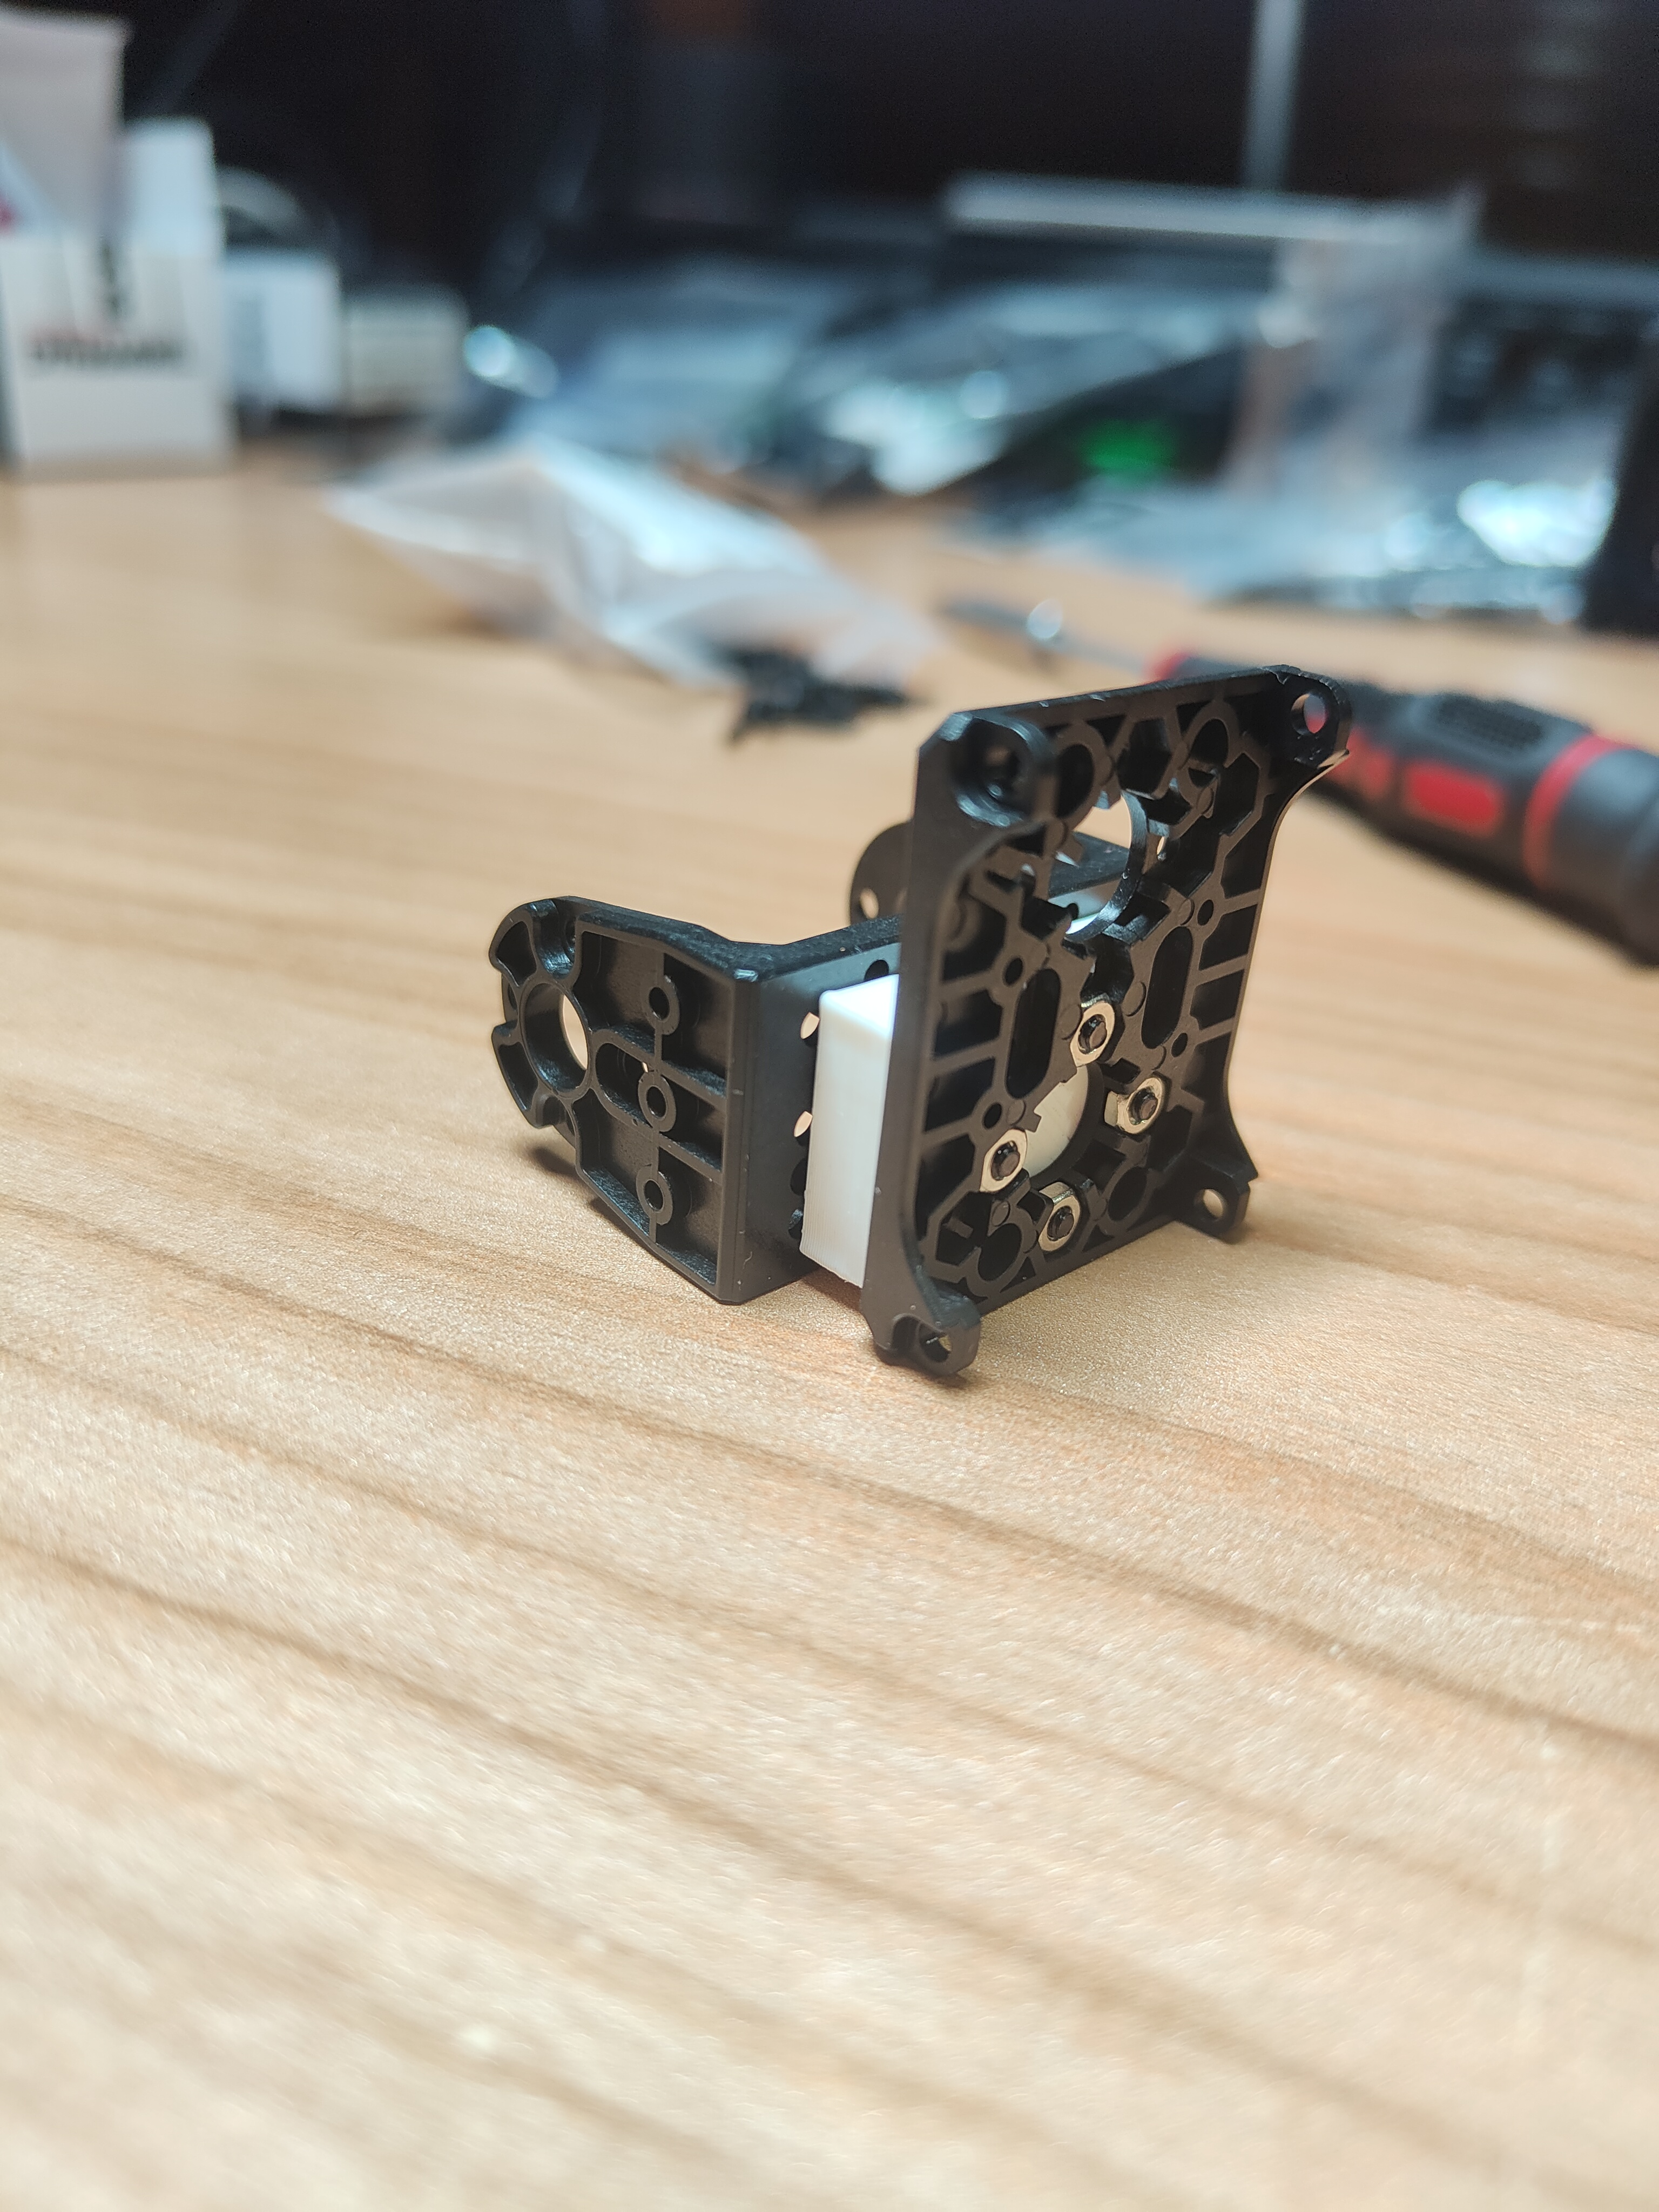
\includegraphics[width=0.25\textwidth]{figs/appendix/dedo/8.jpg} &
  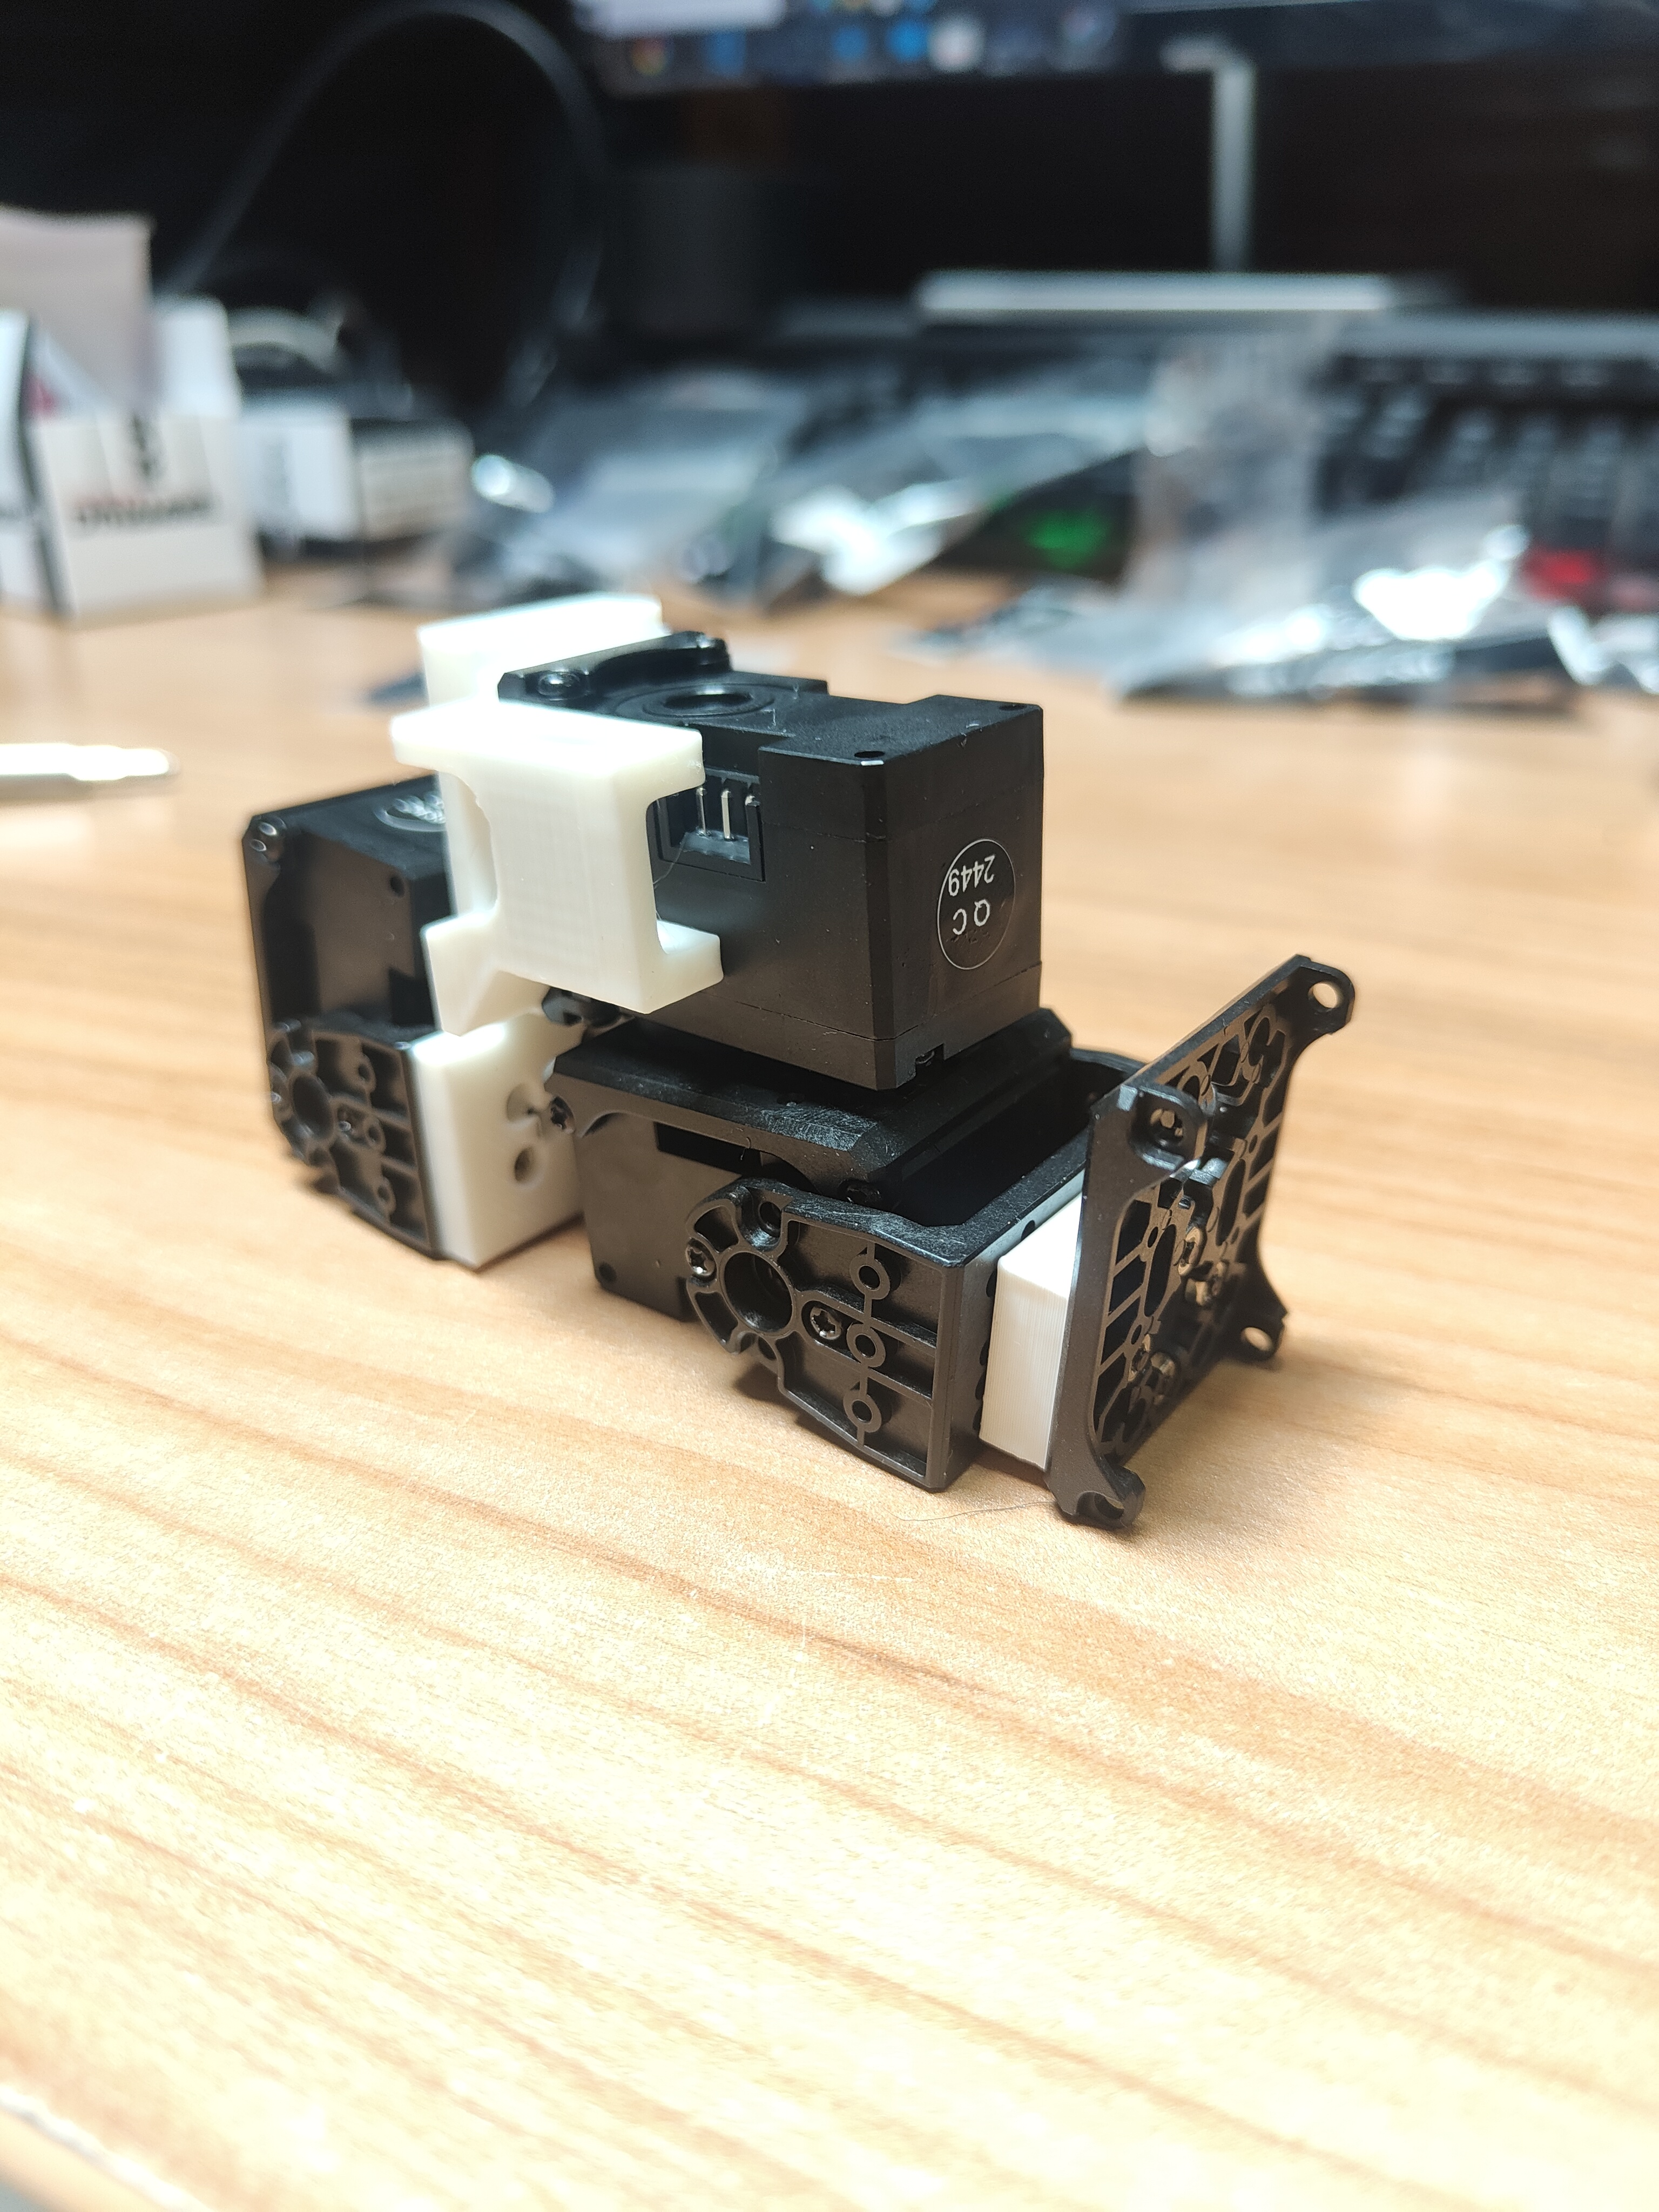
\includegraphics[width=0.25\textwidth]{figs/appendix/dedo/9.jpg} \\
  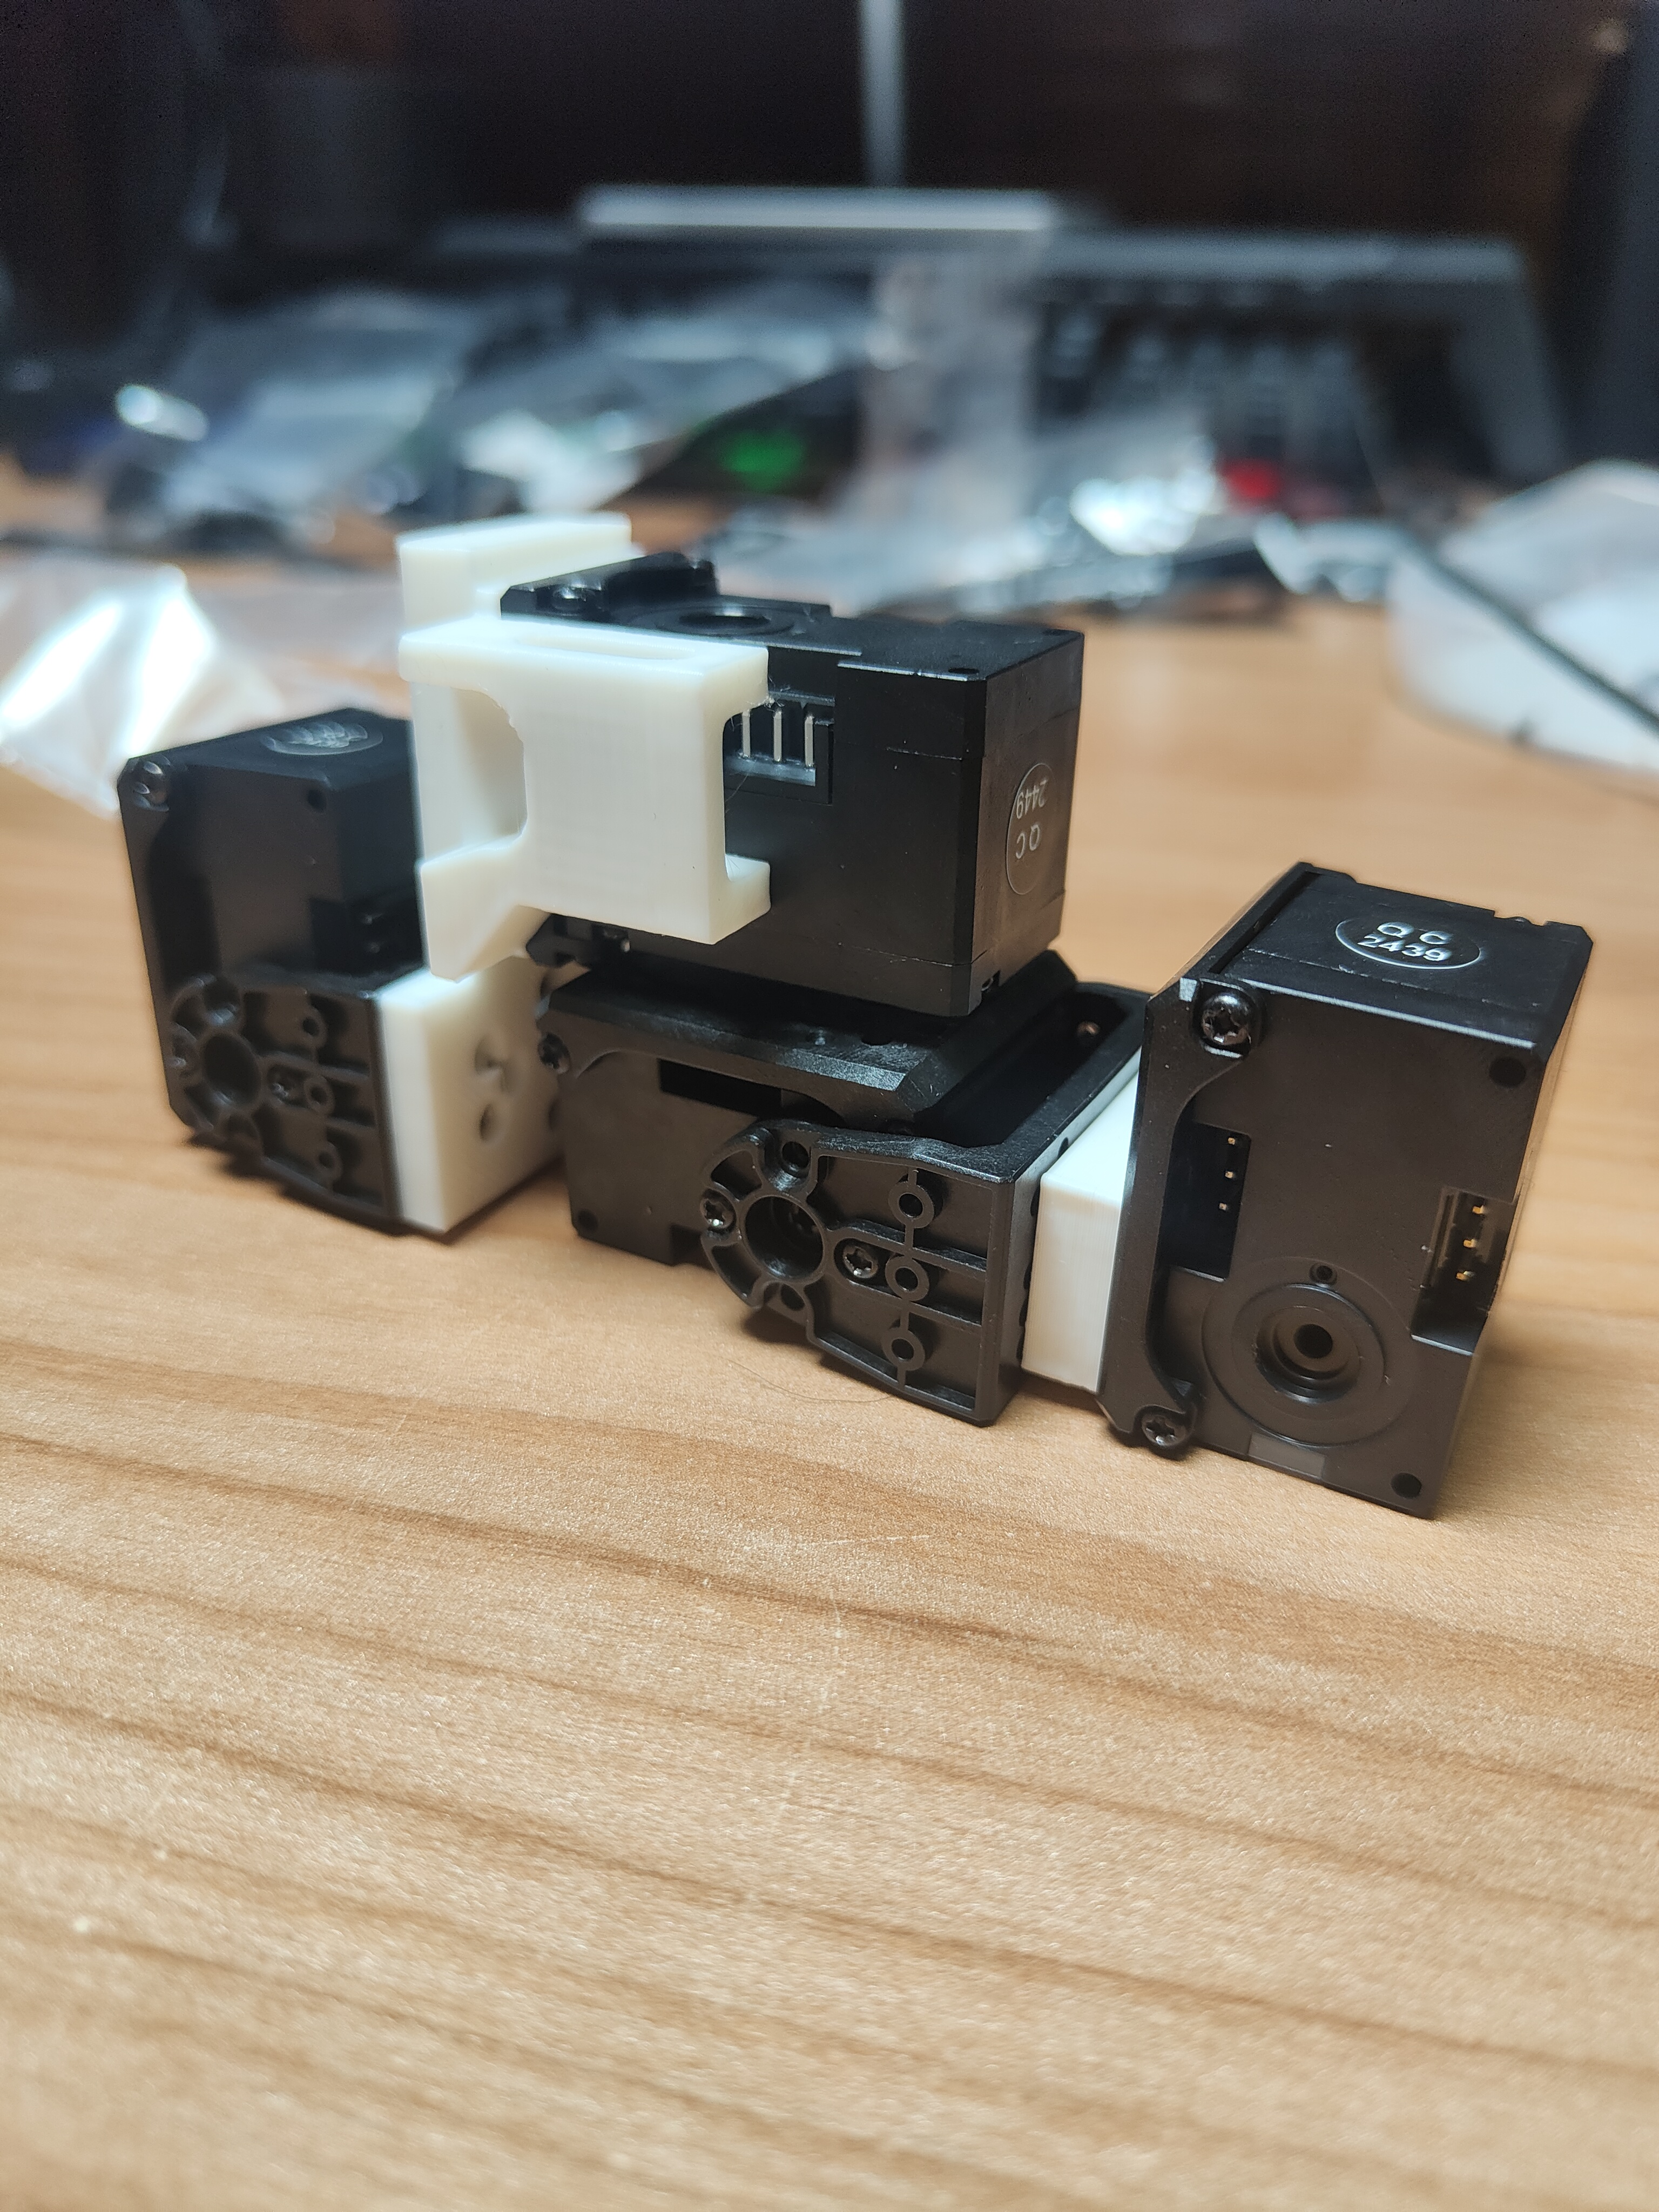
\includegraphics[width=0.25\textwidth]{figs/appendix/dedo/10.jpg} &
  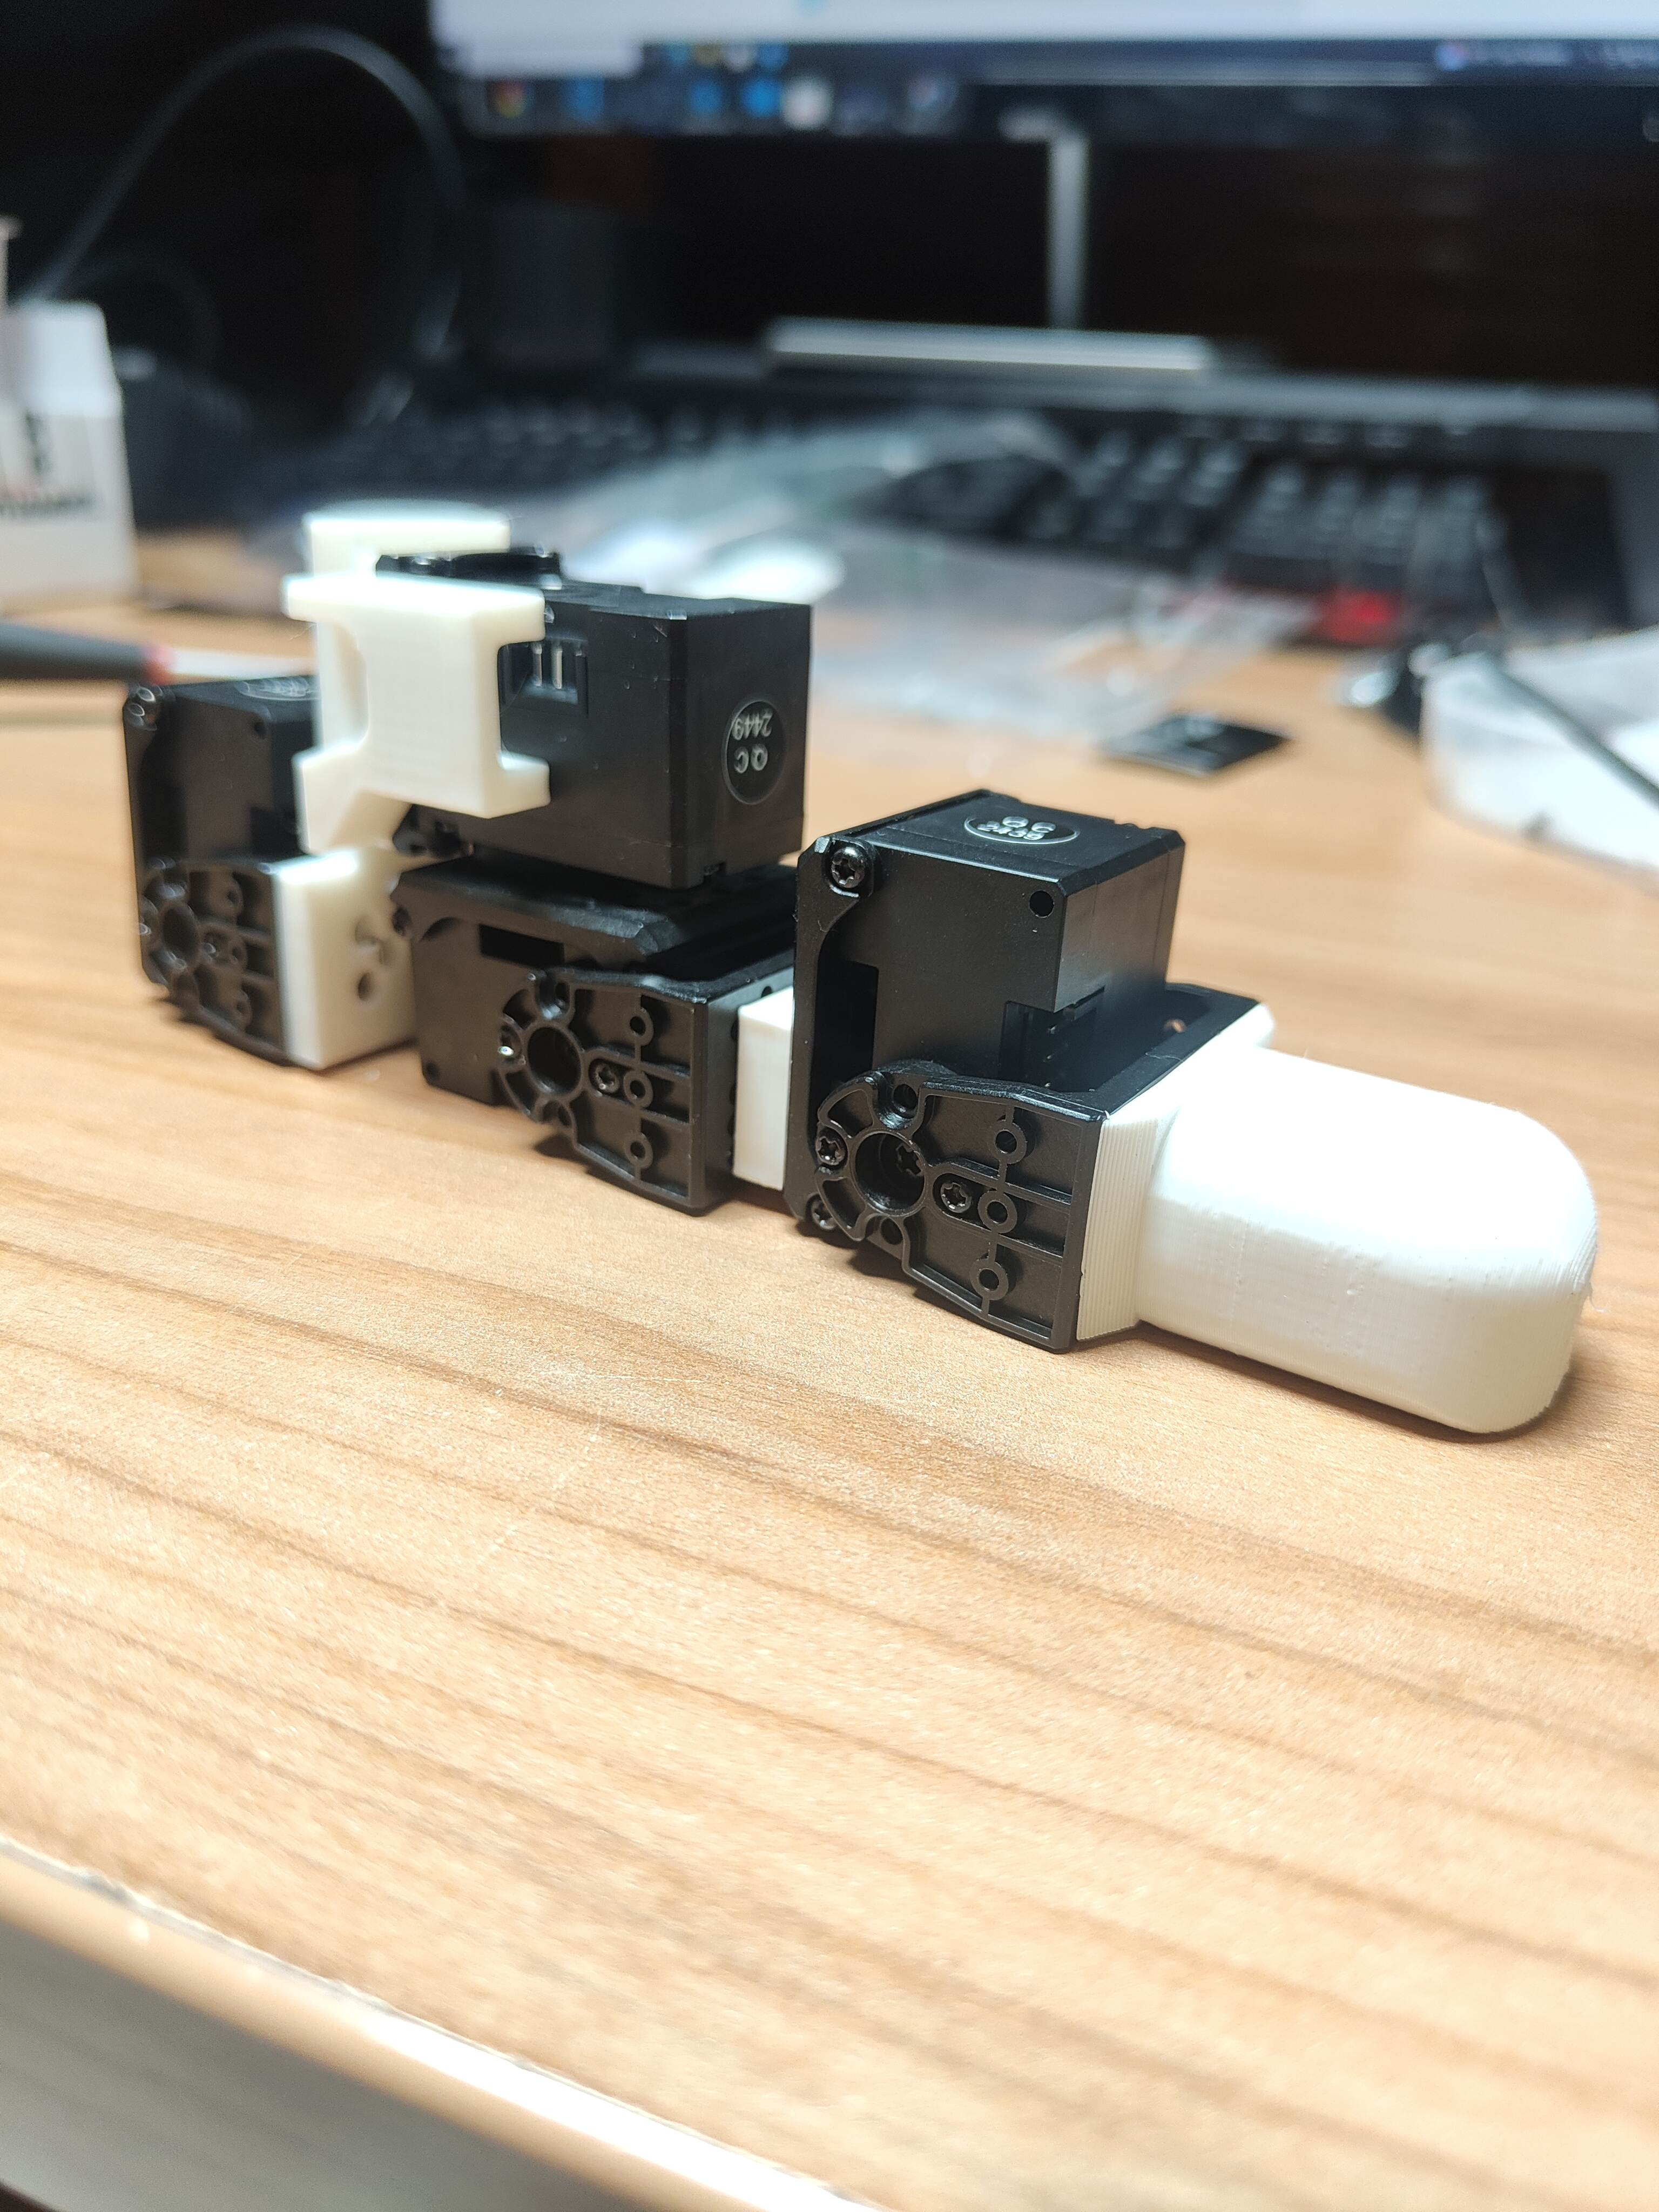
\includegraphics[width=0.25\textwidth]{figs/appendix/dedo/11.jpg} &
\end{tabular}
\caption{Fotografias sequenciais da montagem do dedo referente ao dedo indicador, médio ou anelar}
\end{figure}

\label{appendix:montagem_dedo}

\subsection{Hiperligações}

\label{appendix:videos}

\section{Testes realizados com um dedo}

\subsection{Teste com duas velocidades diferentes}

\begin{figure}[H]
\centering
\begin{tabular}{ccc}
  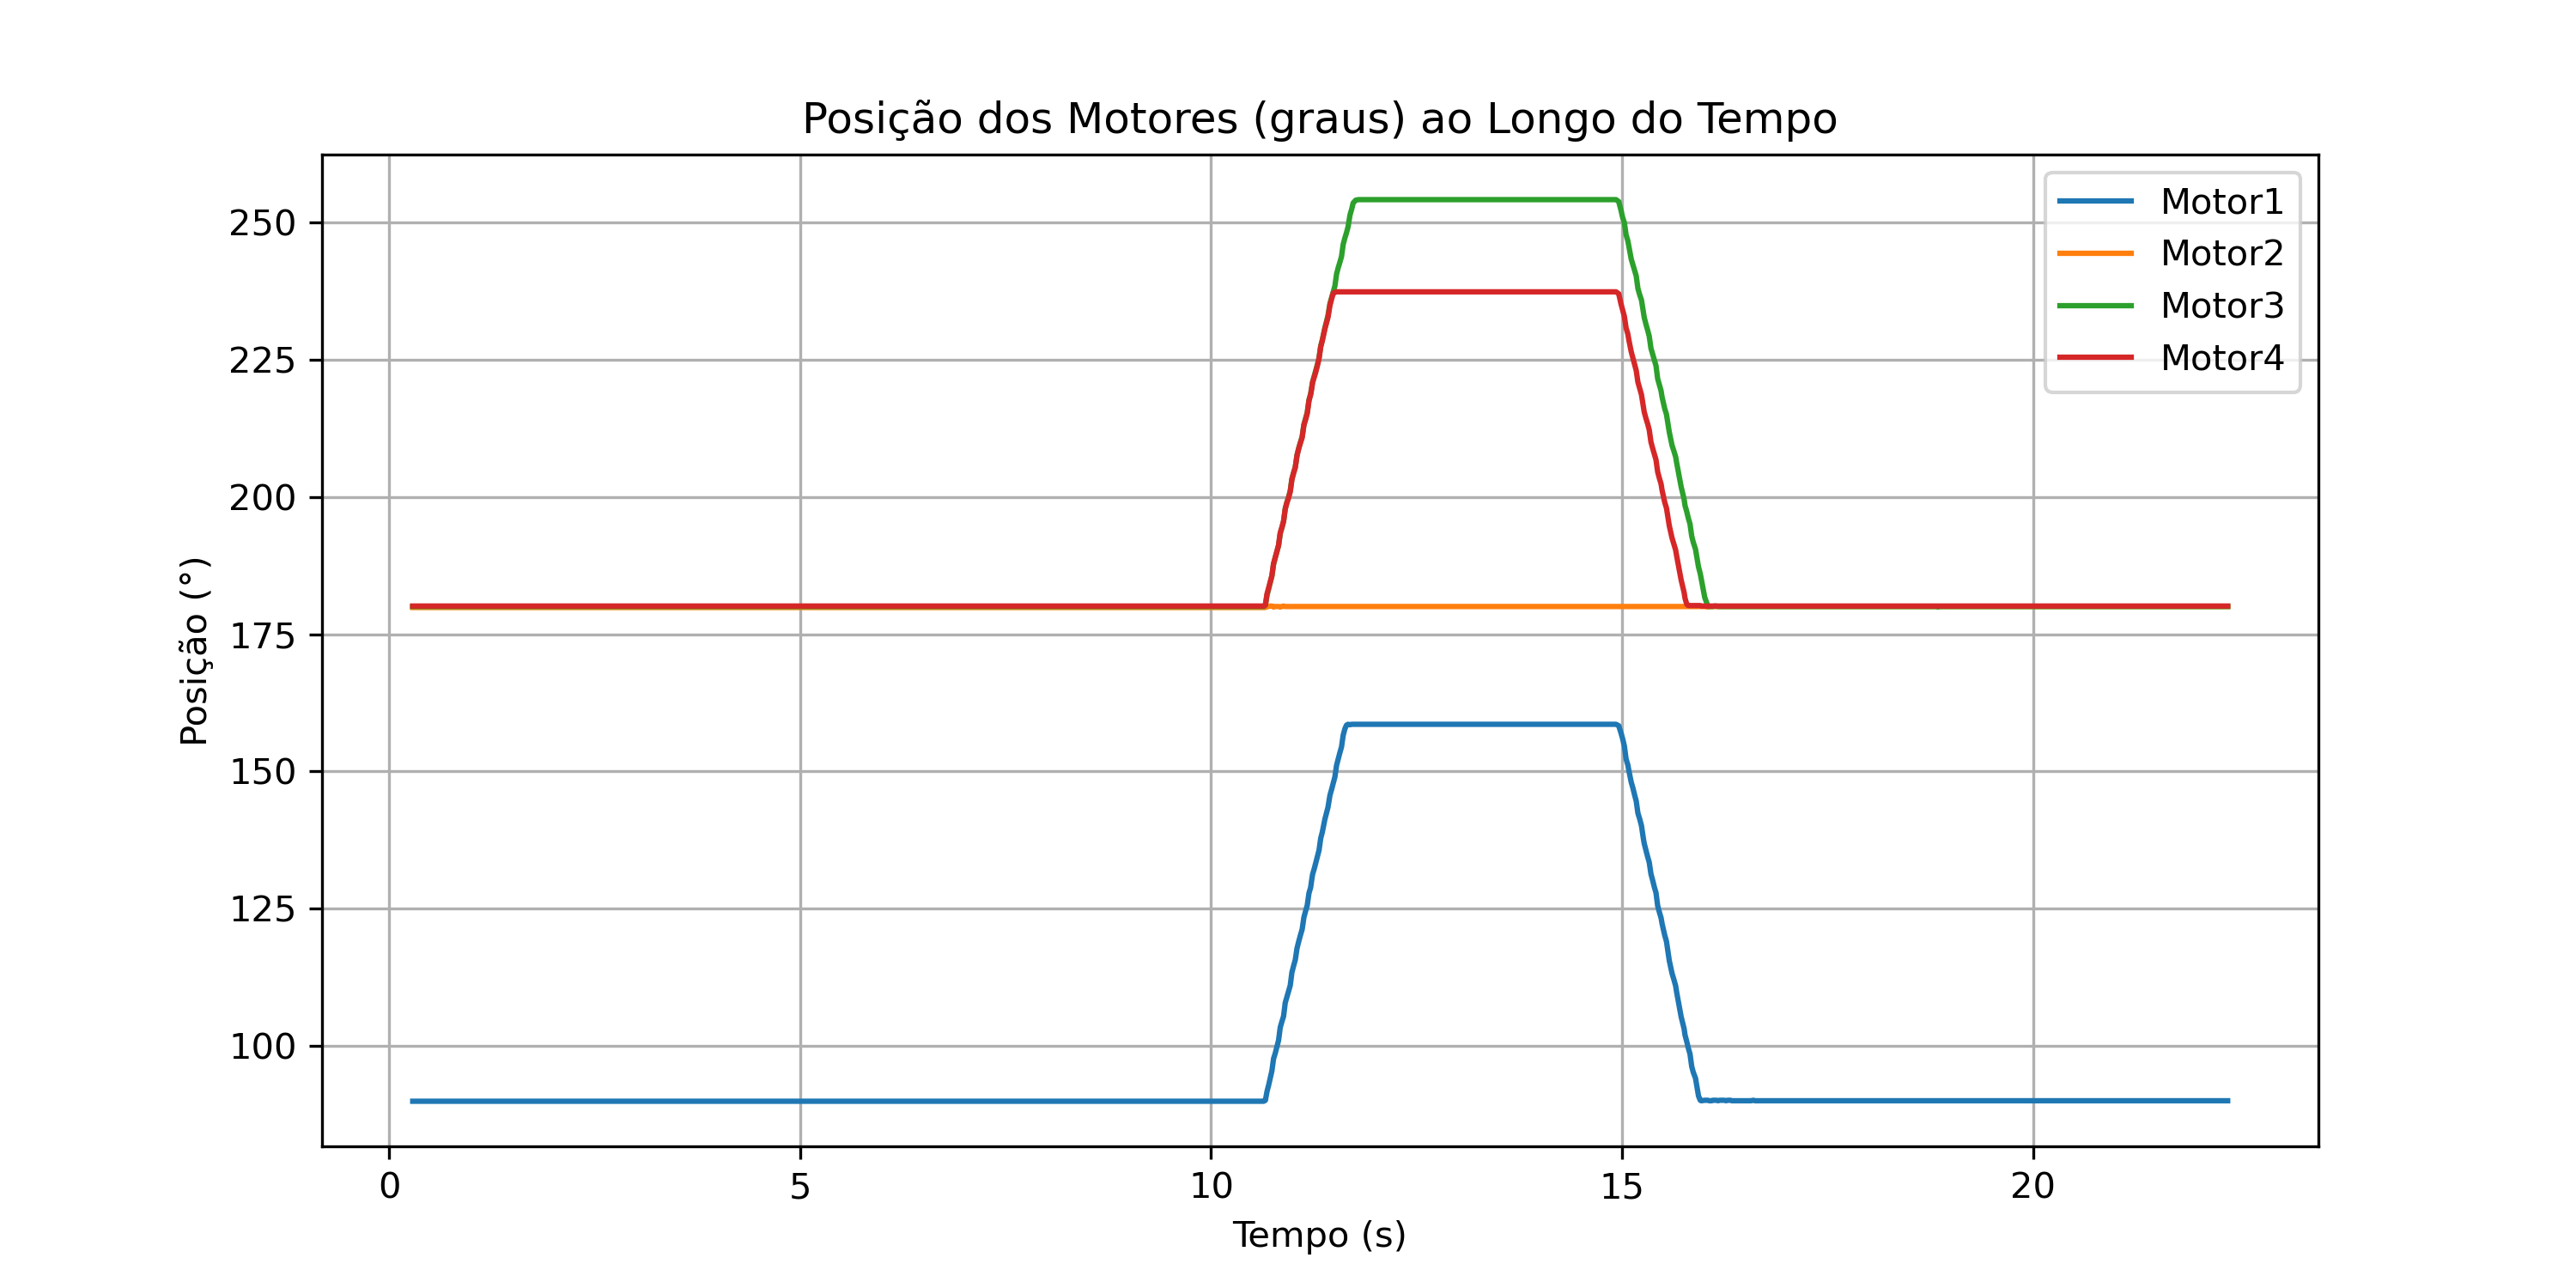
\includegraphics[width=0.5\textwidth]{figs/appendix/teste_velocidades/finger_positions_vel50.png} &
  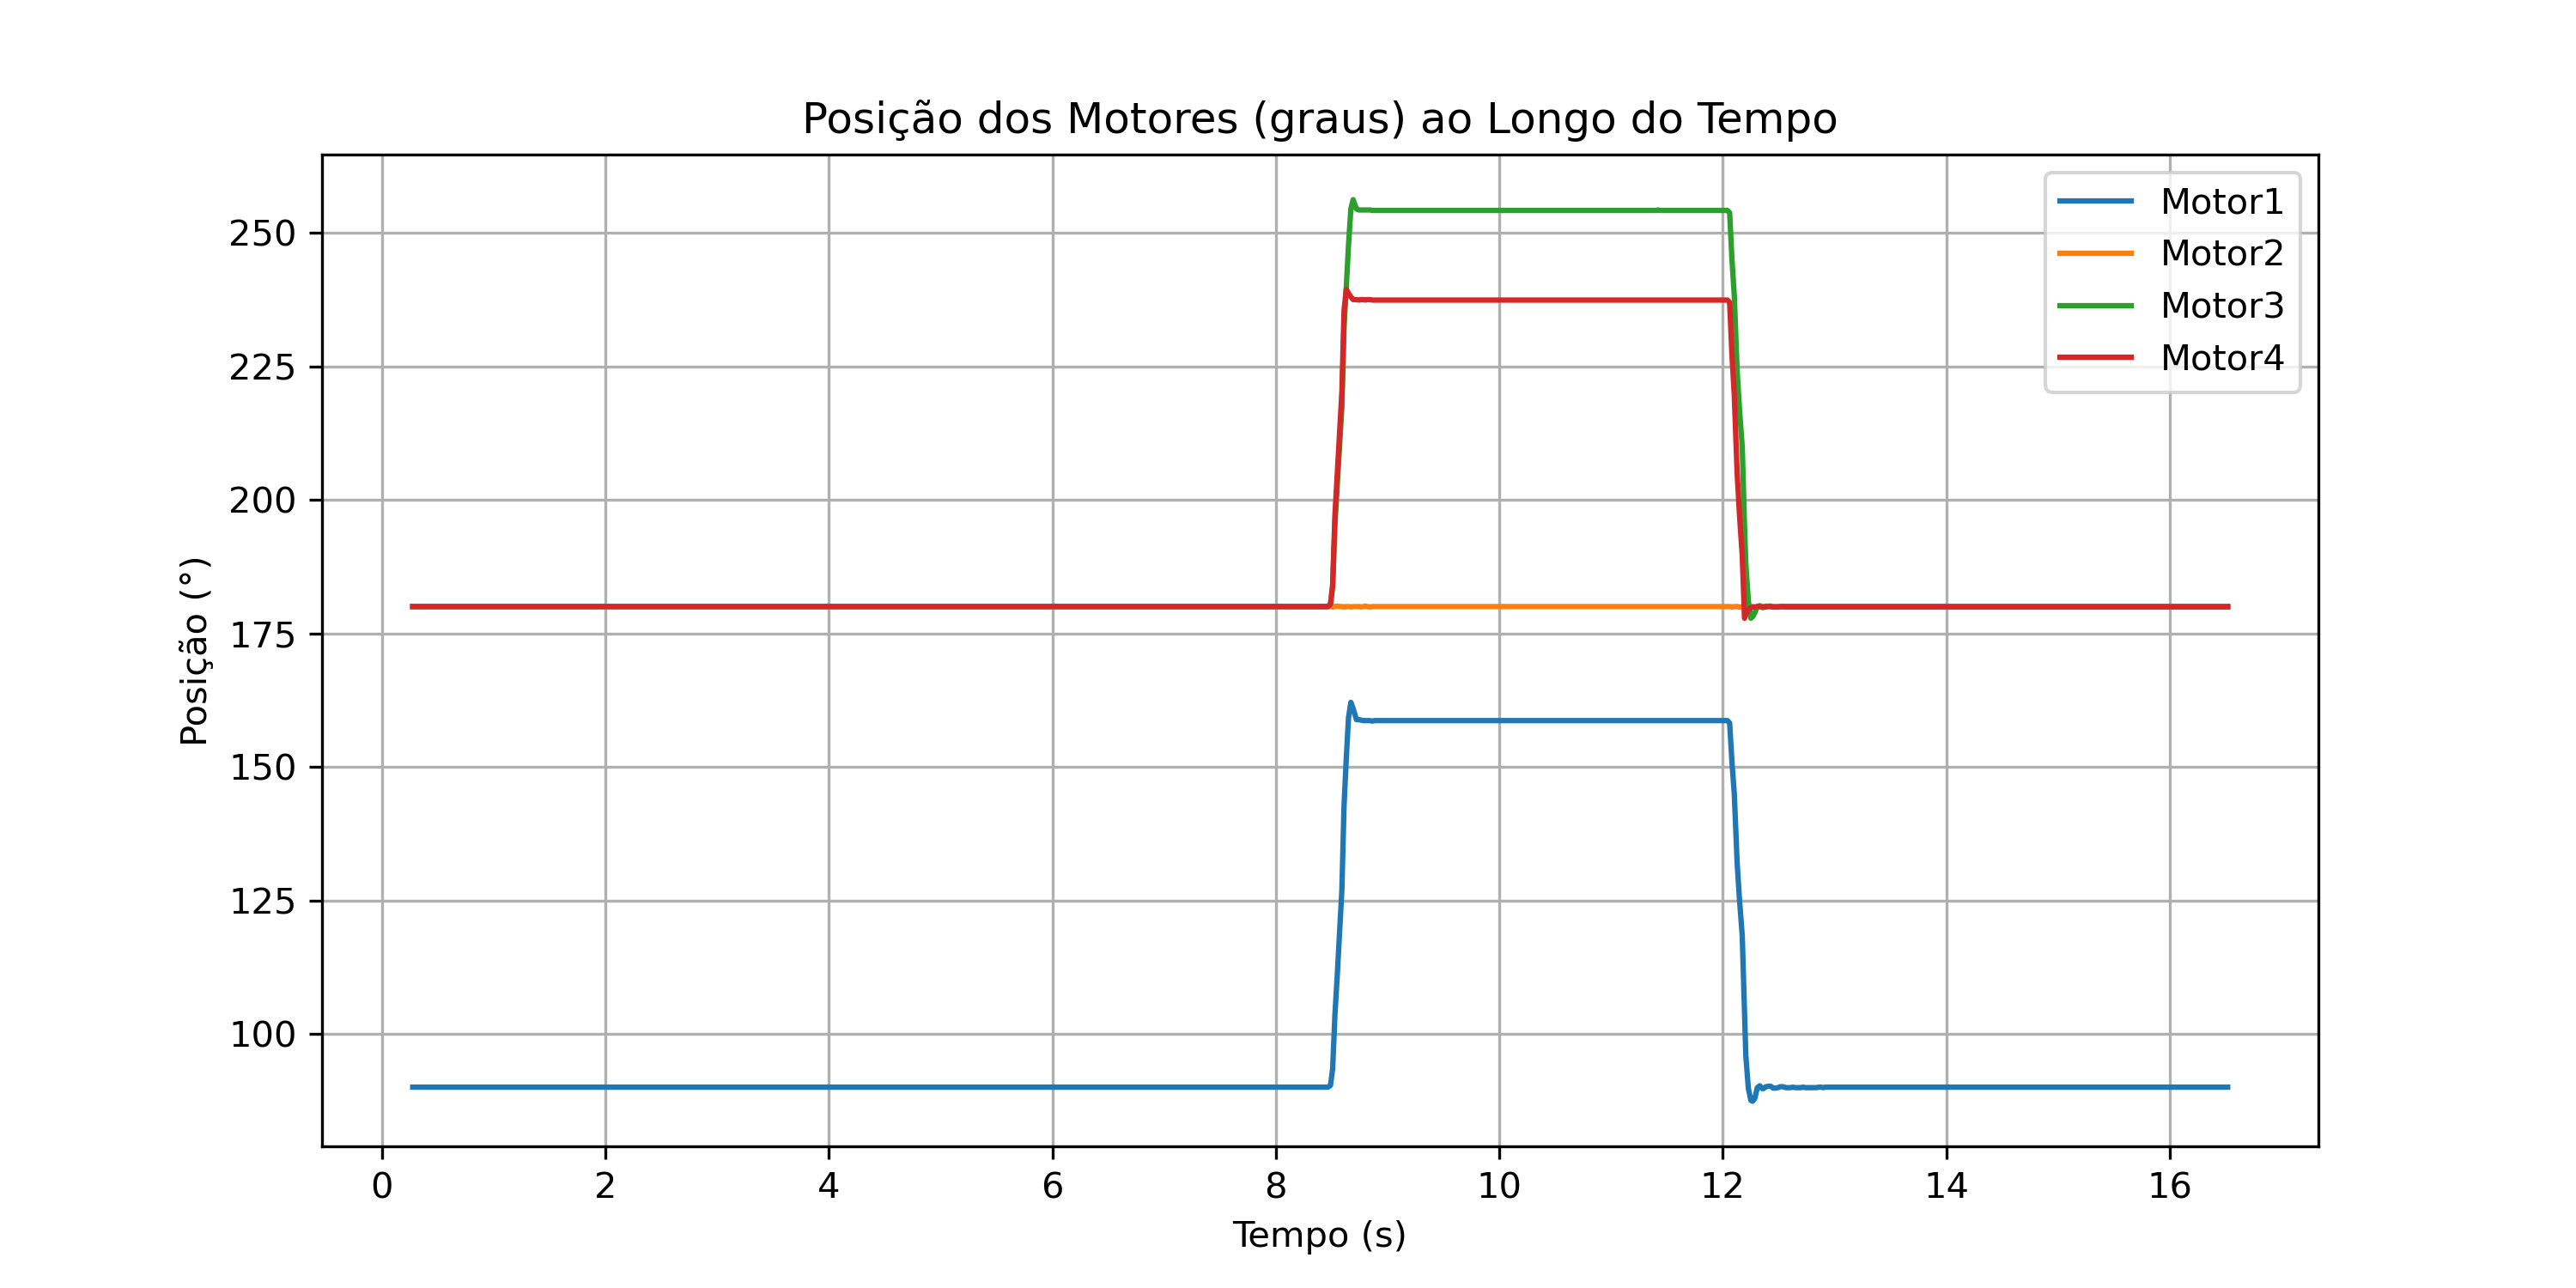
\includegraphics[width=0.5\textwidth]{figs/appendix/teste_velocidades/finger_positions_vel1000.png} \\
  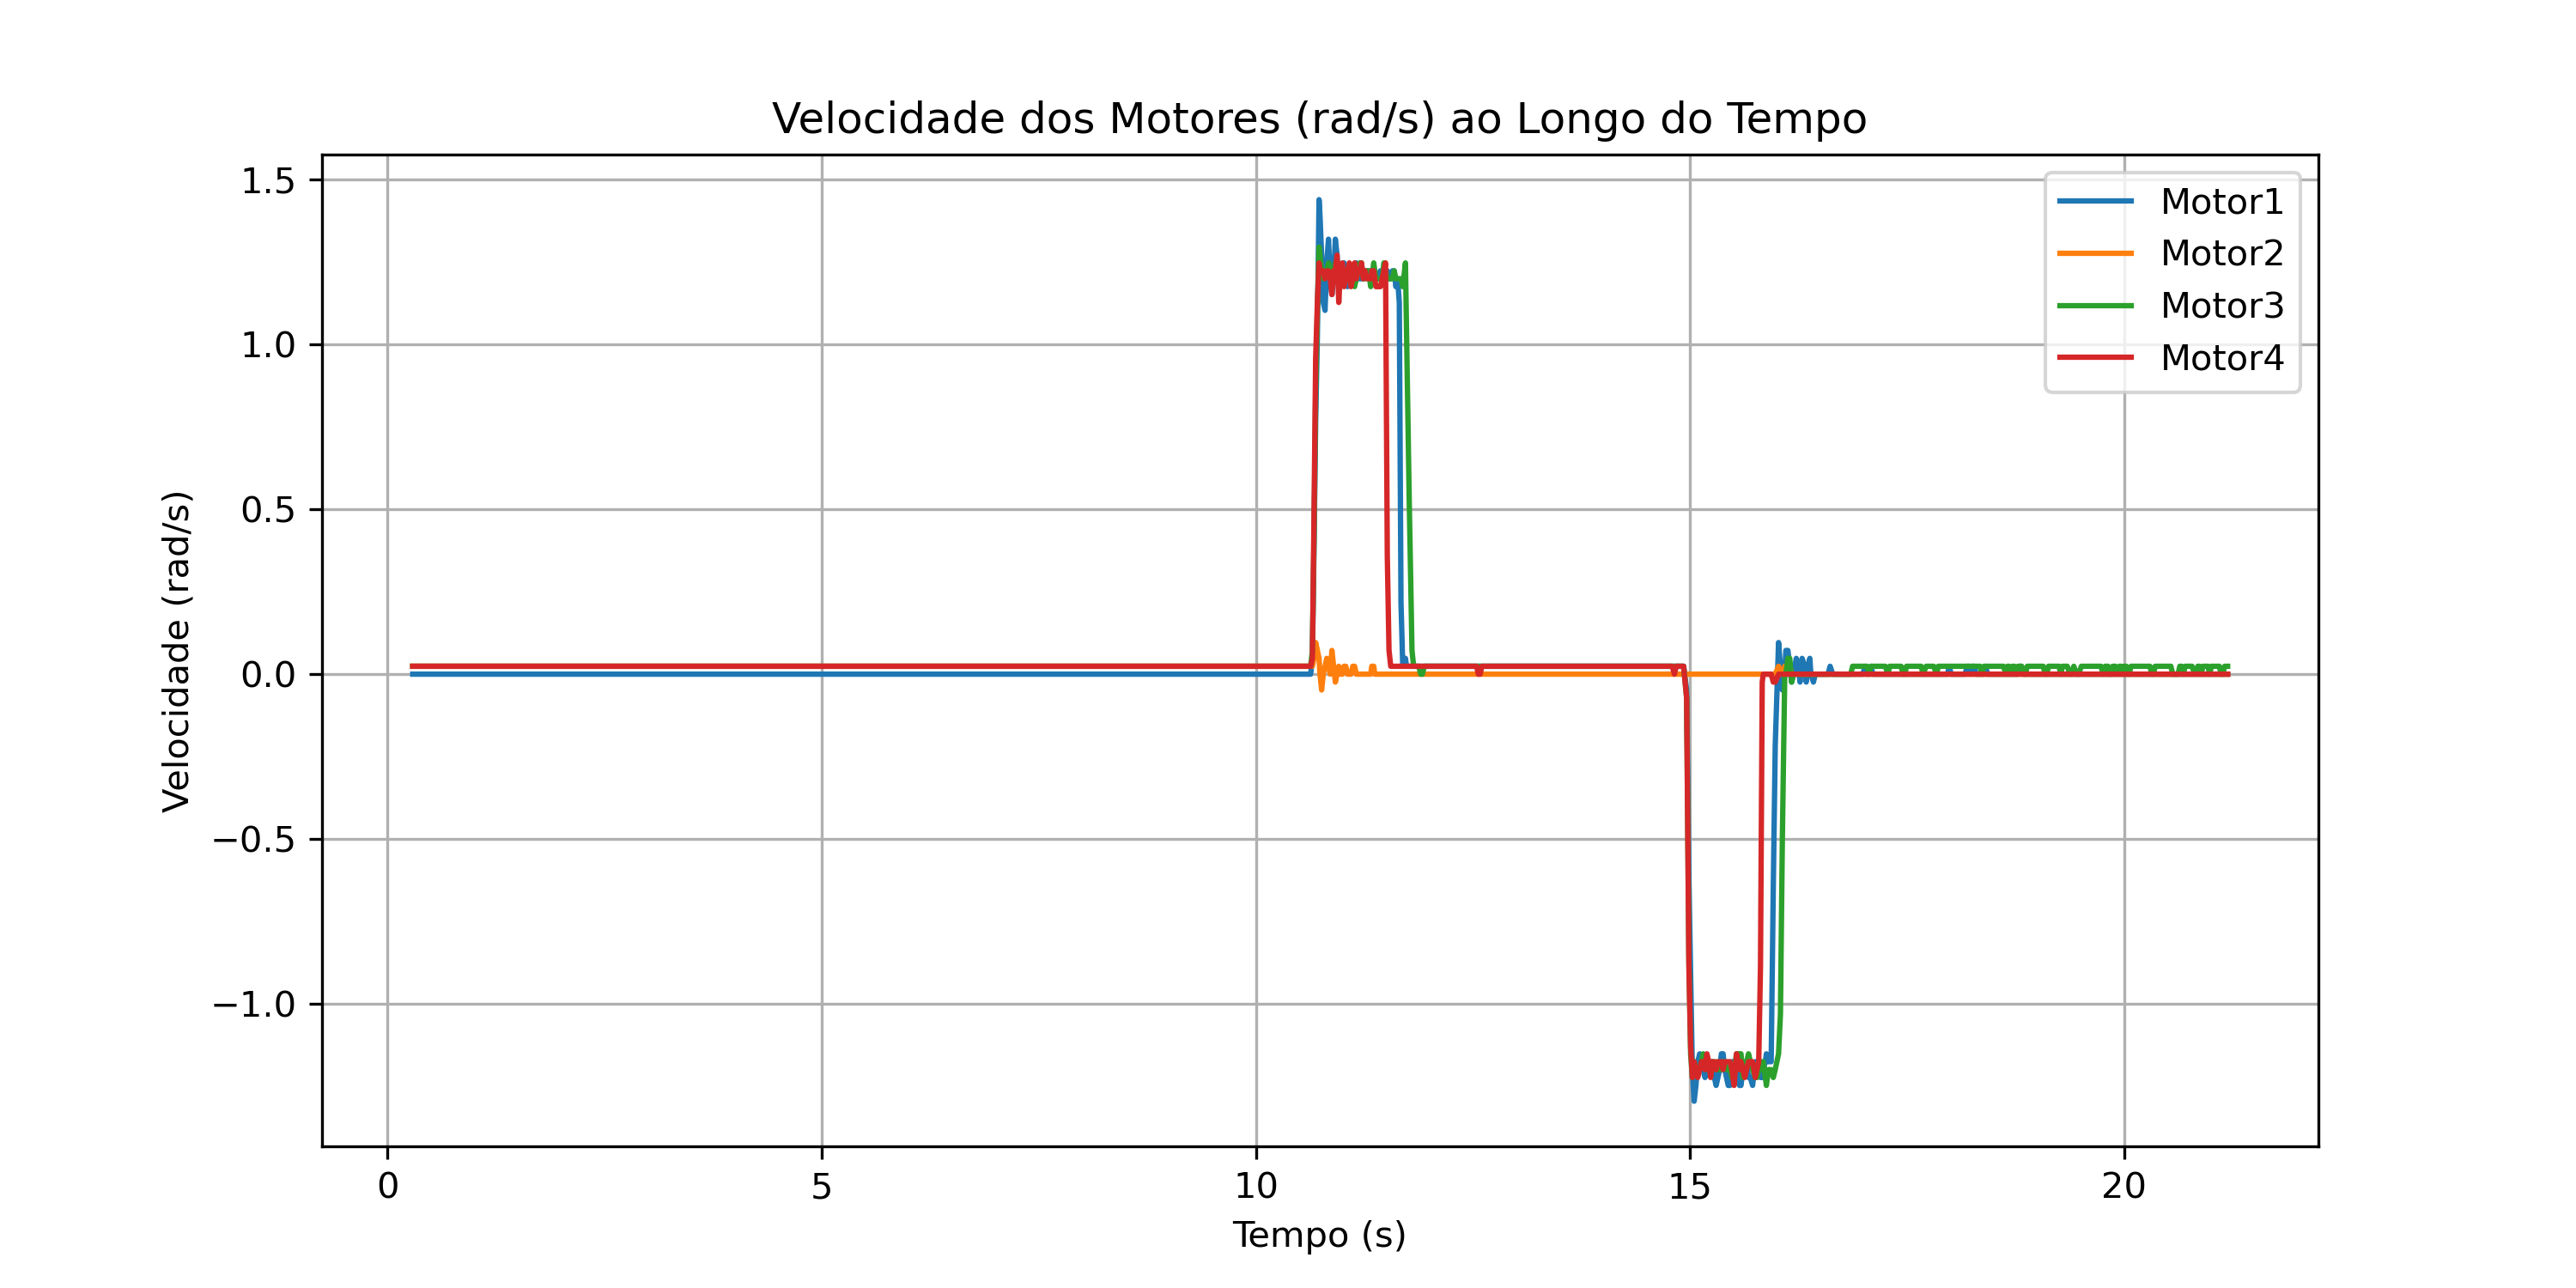
\includegraphics[width=0.5\textwidth]{figs/appendix/teste_velocidades/finger_velocities_vel50.png} &
  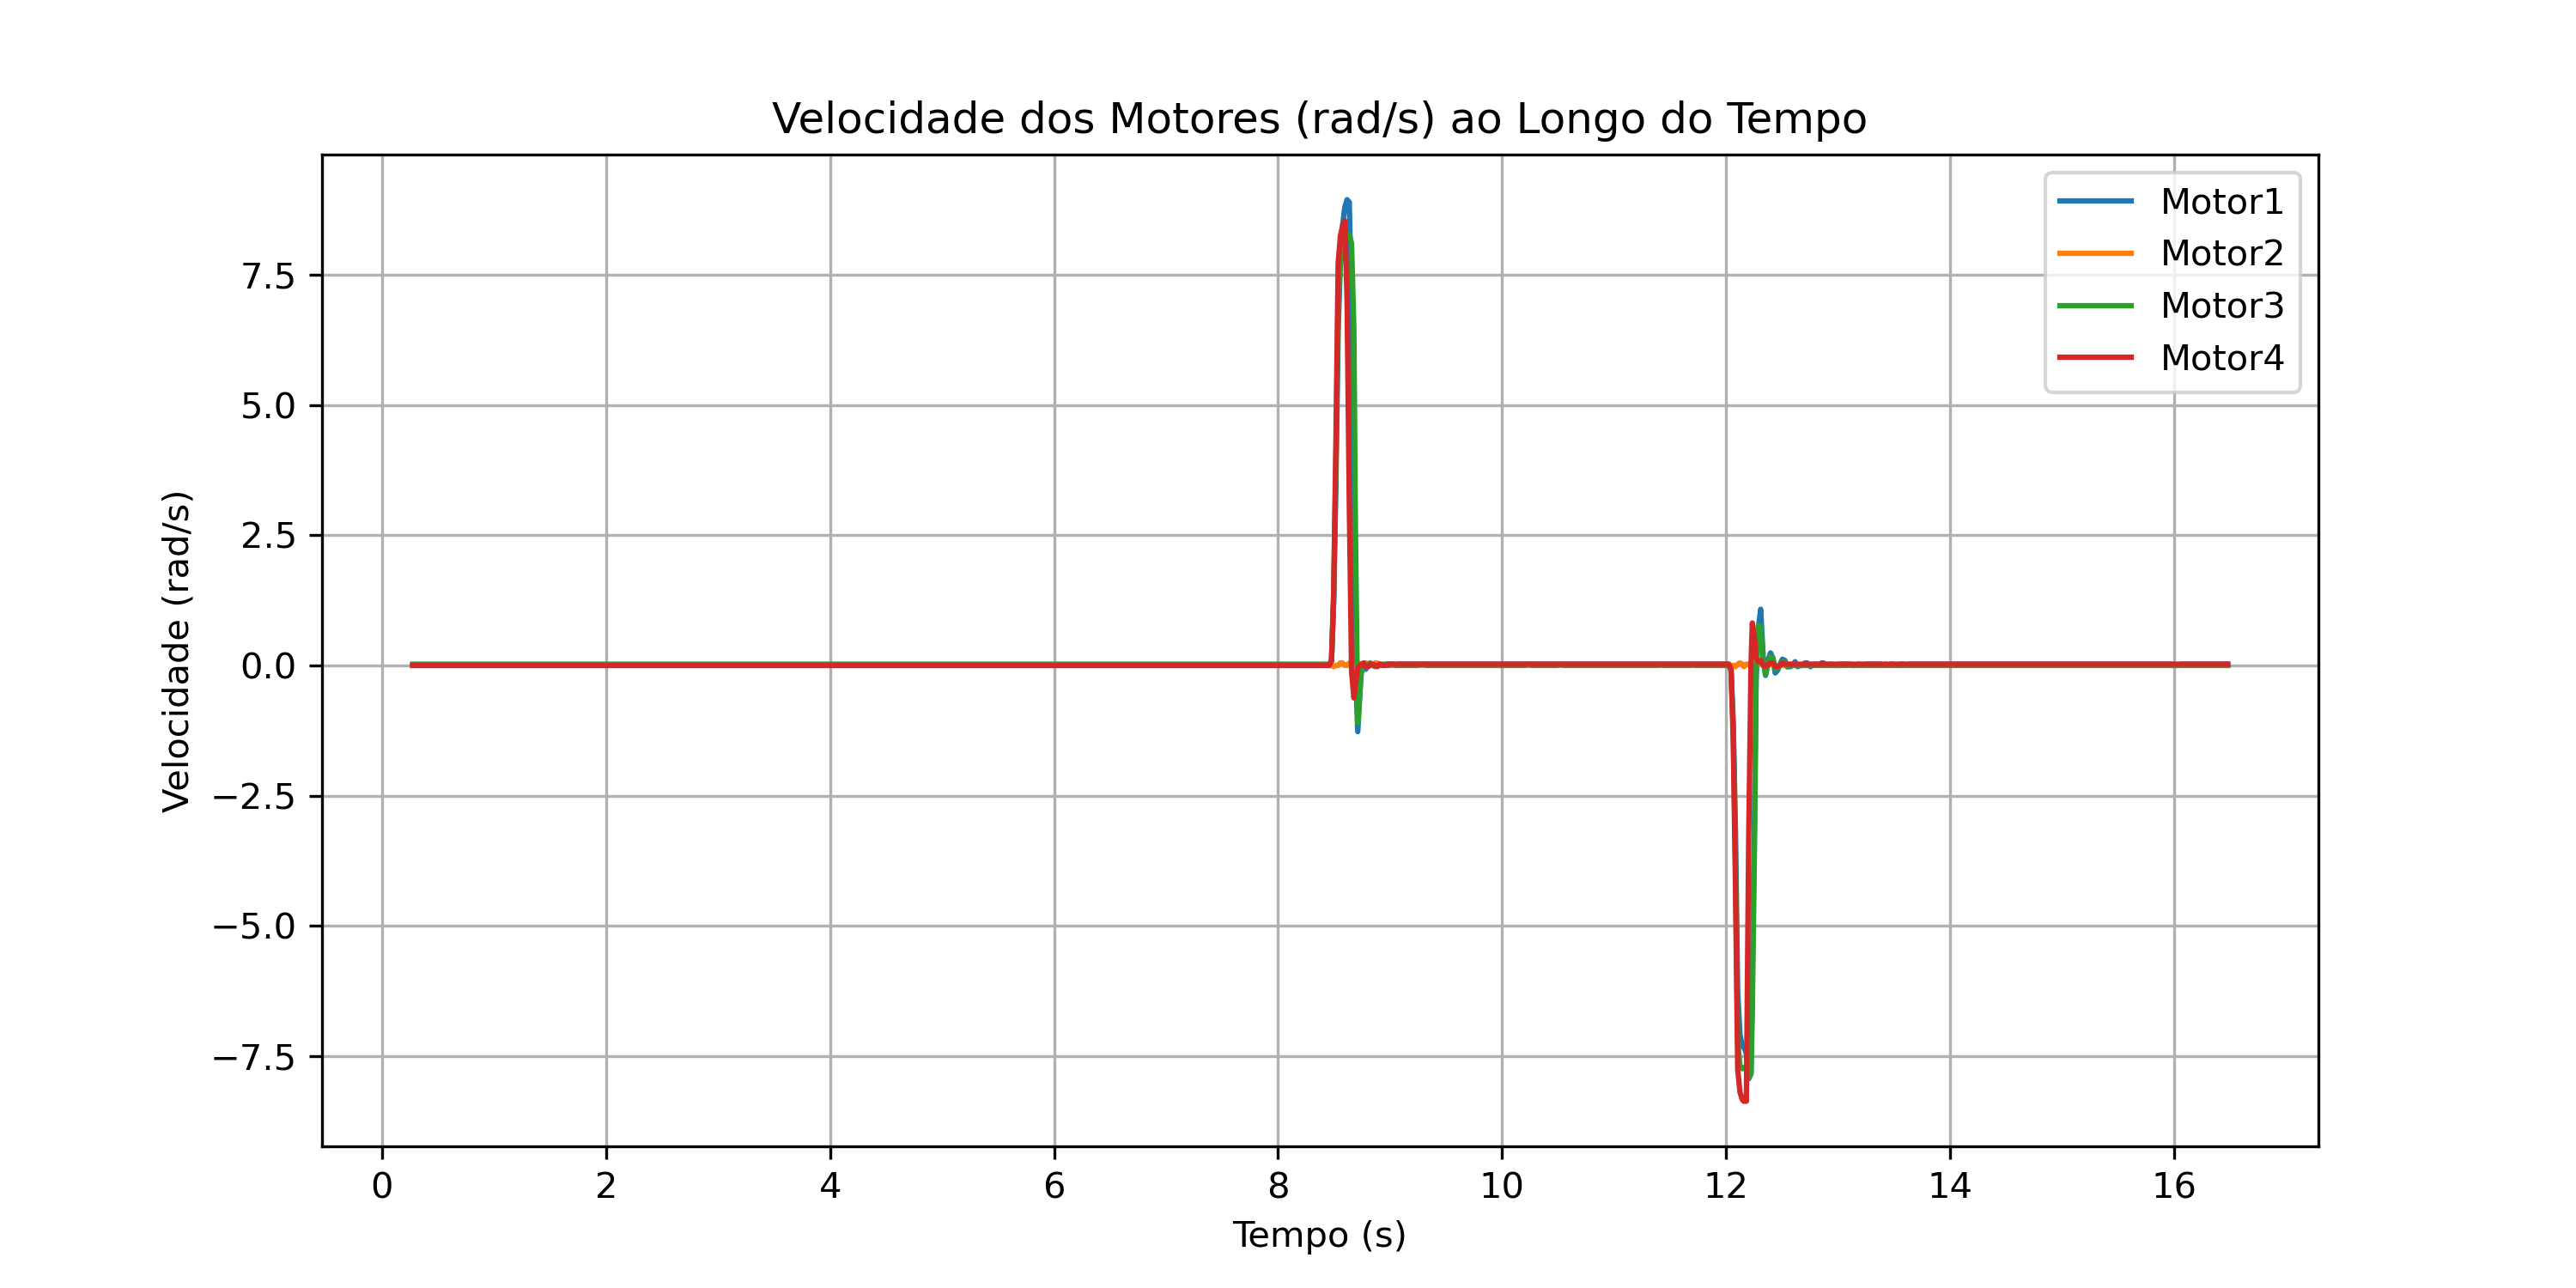
\includegraphics[width=0.5\textwidth]{figs/appendix/teste_velocidades/finger_velocities_vel1000.png} \\
  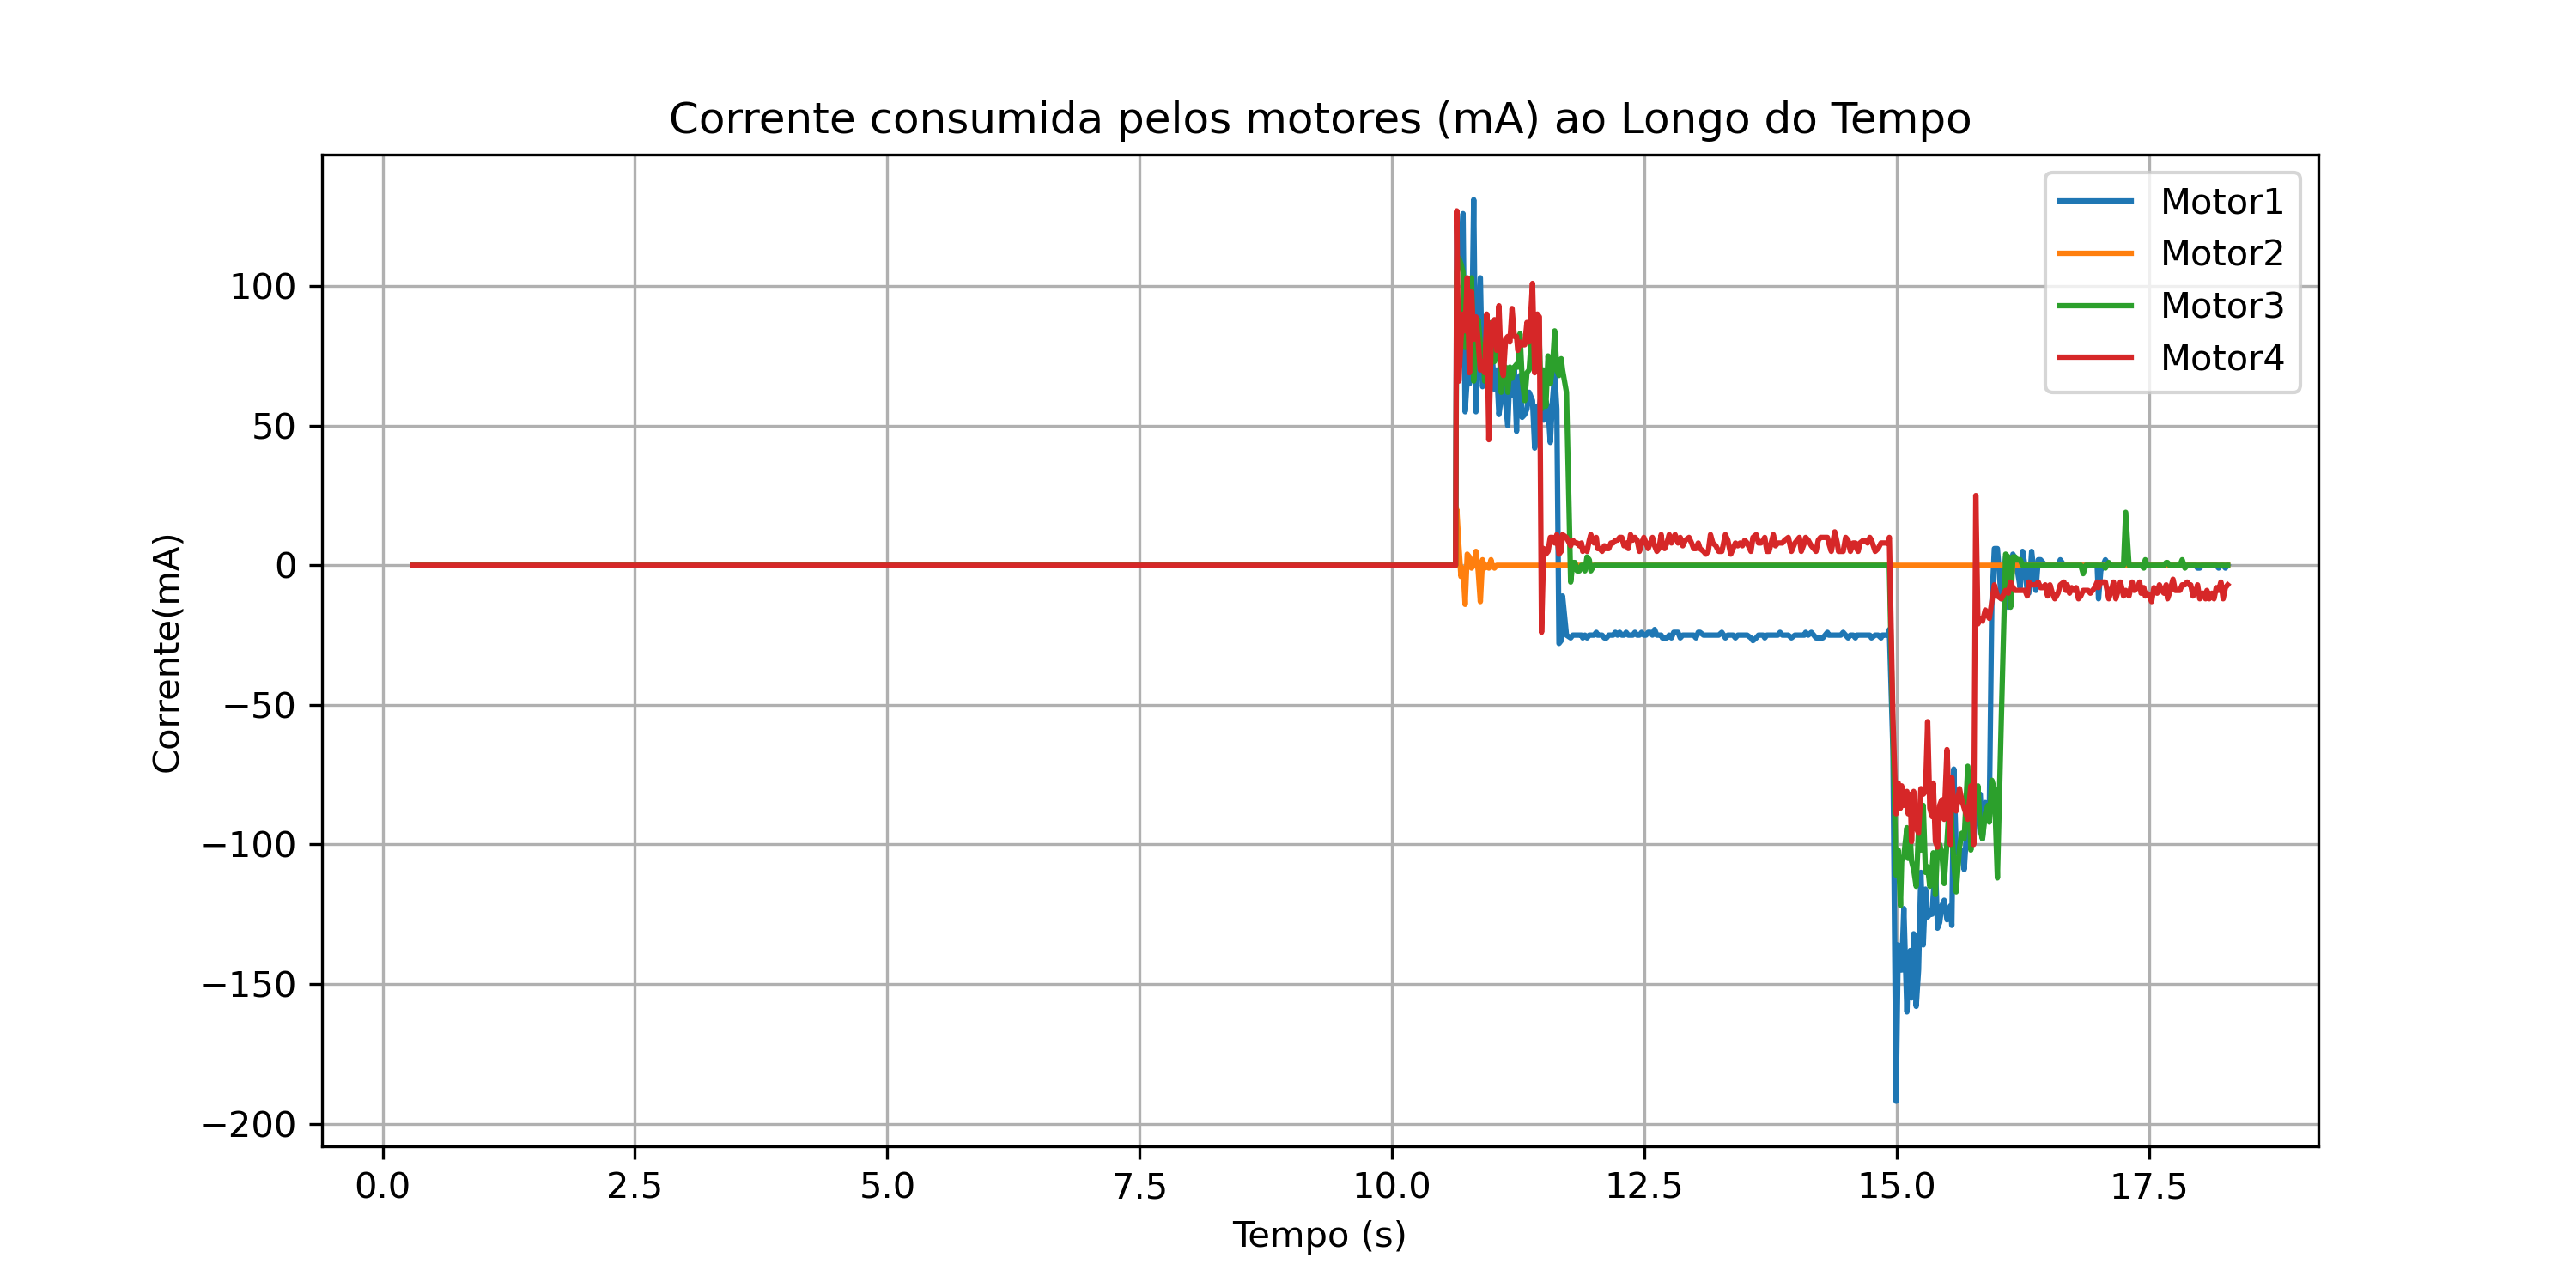
\includegraphics[width=0.5\textwidth]{figs/appendix/teste_velocidades/finger_currents_vel50.png} &
  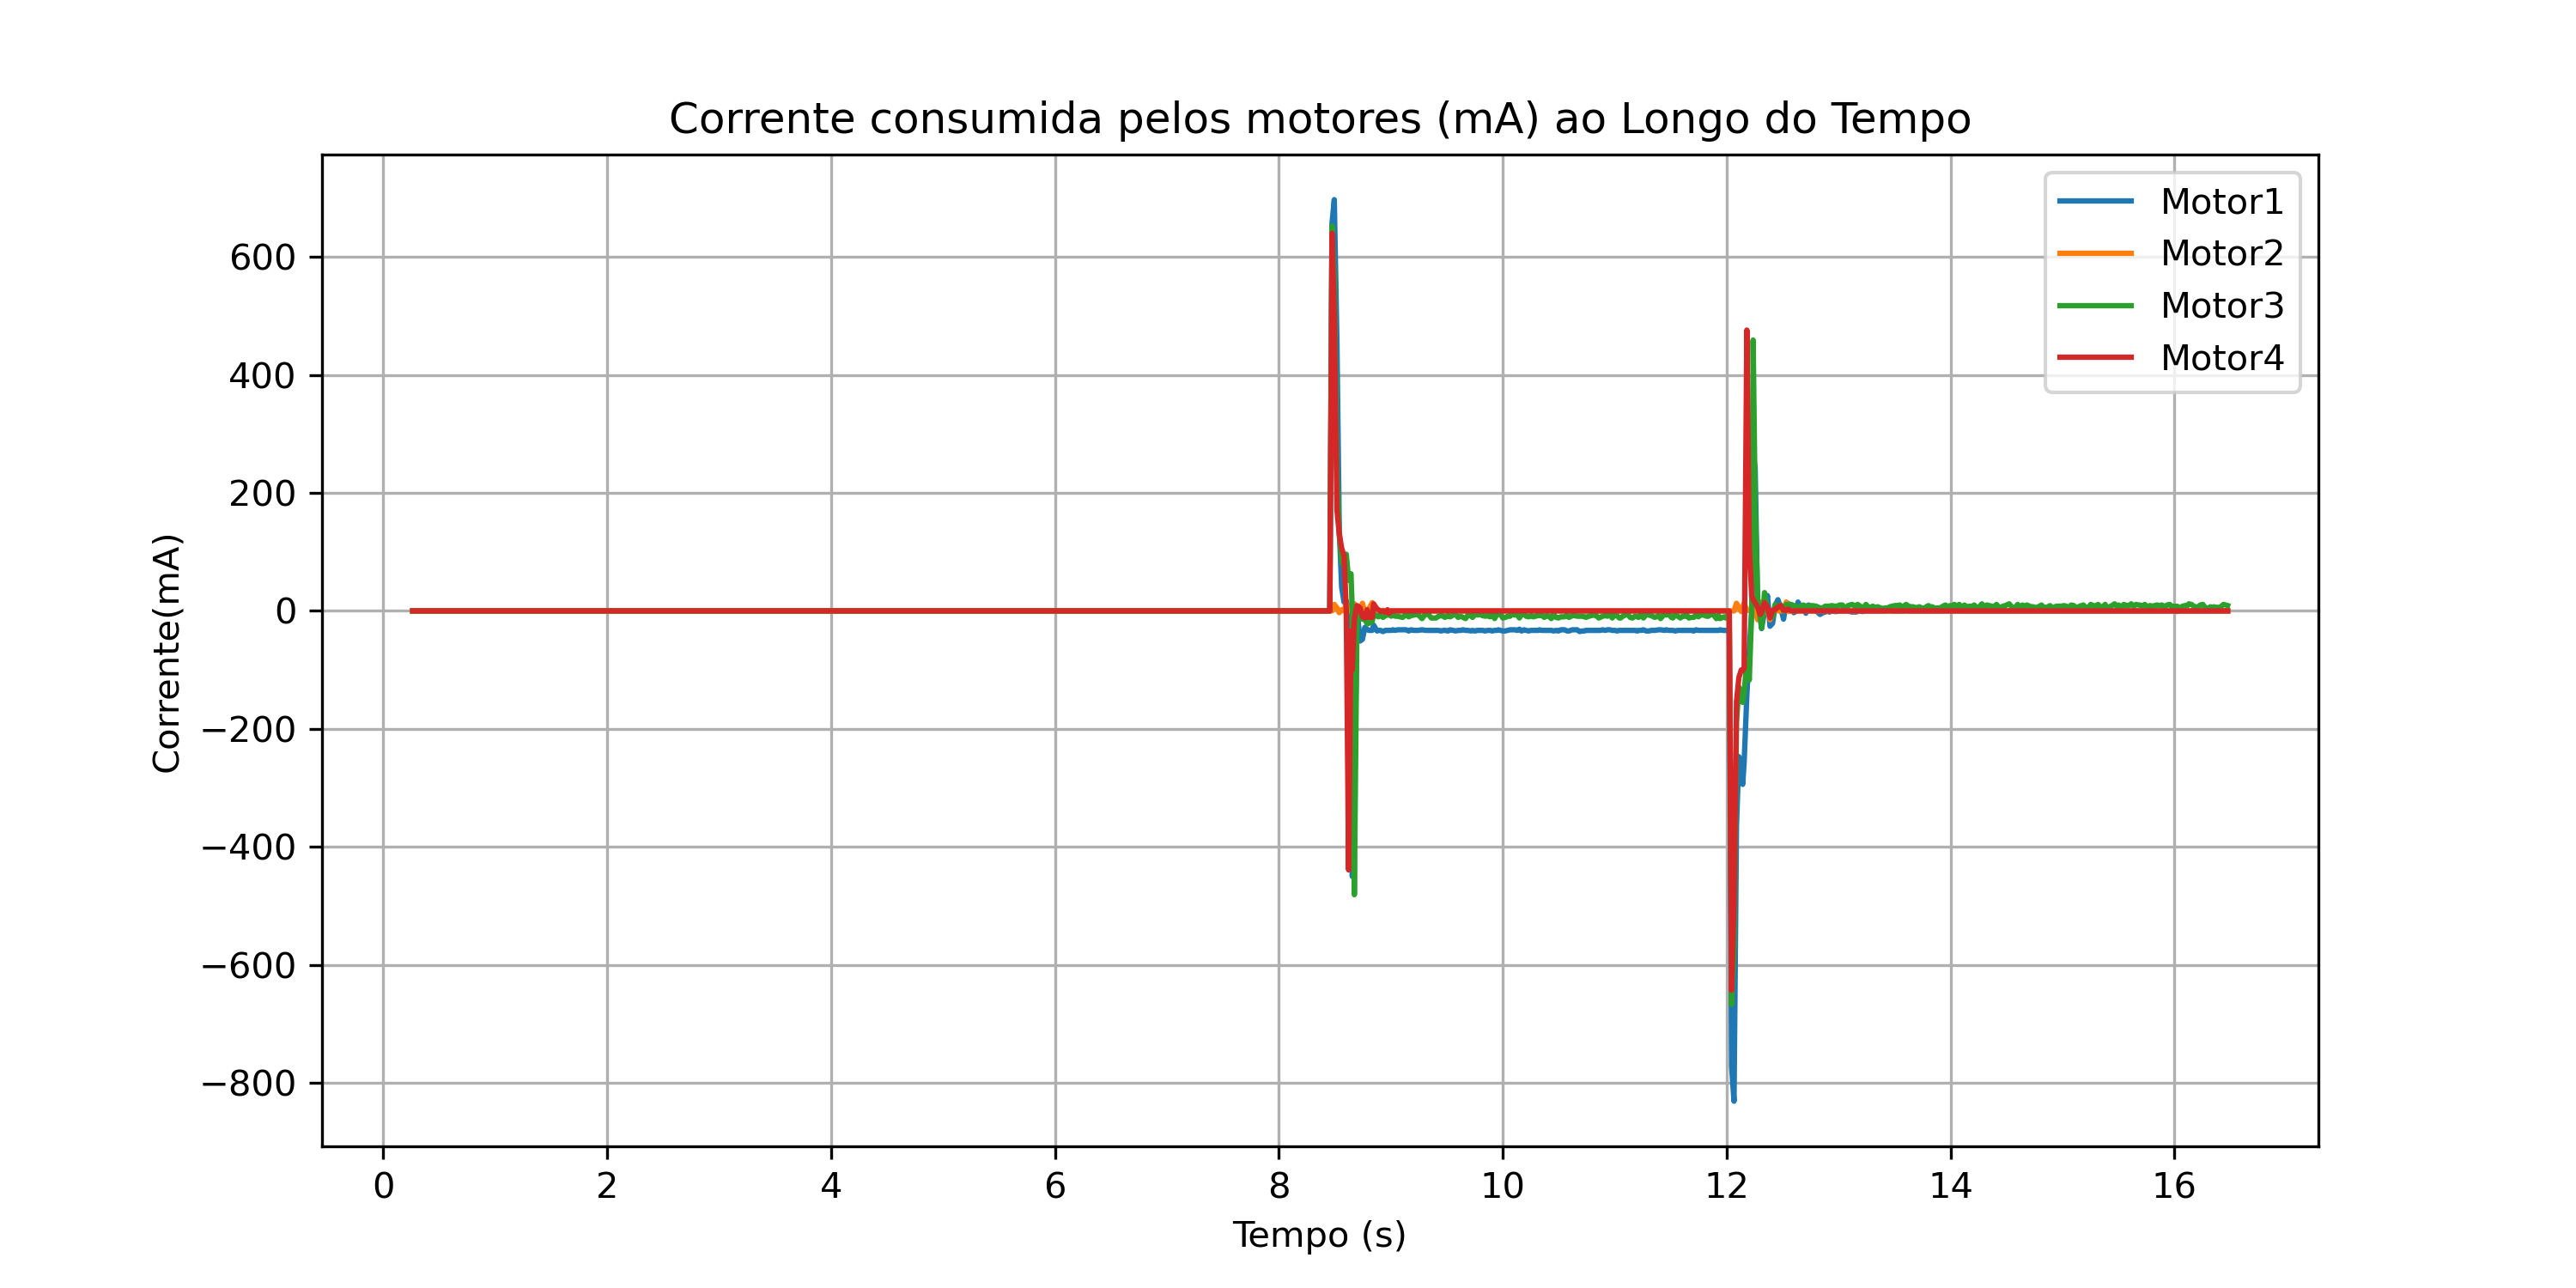
\includegraphics[width=0.5\textwidth]{figs/appendix/teste_velocidades/finger_currents_vel1000.png} \\
\end{tabular}
\caption{Gráficos da posição, velocidade e corrente consumida pelos motores de um dedo. A coluna da esquerda corresponde a uma velocidade máxima configurada de 1.2 rad/s e a coluna da direita a 23.98 rad/s.}
\end{figure}

Hiperligação para vídeo: \url{https://www.youtube.com/shorts/_3l9AzUPu9A}

\label{appendix:teste_velocidades}

\subsection{Teste com obstáculo em posições diferentes}

\begin{figure}[H]
\centering
\begin{tabular}{ccc}
  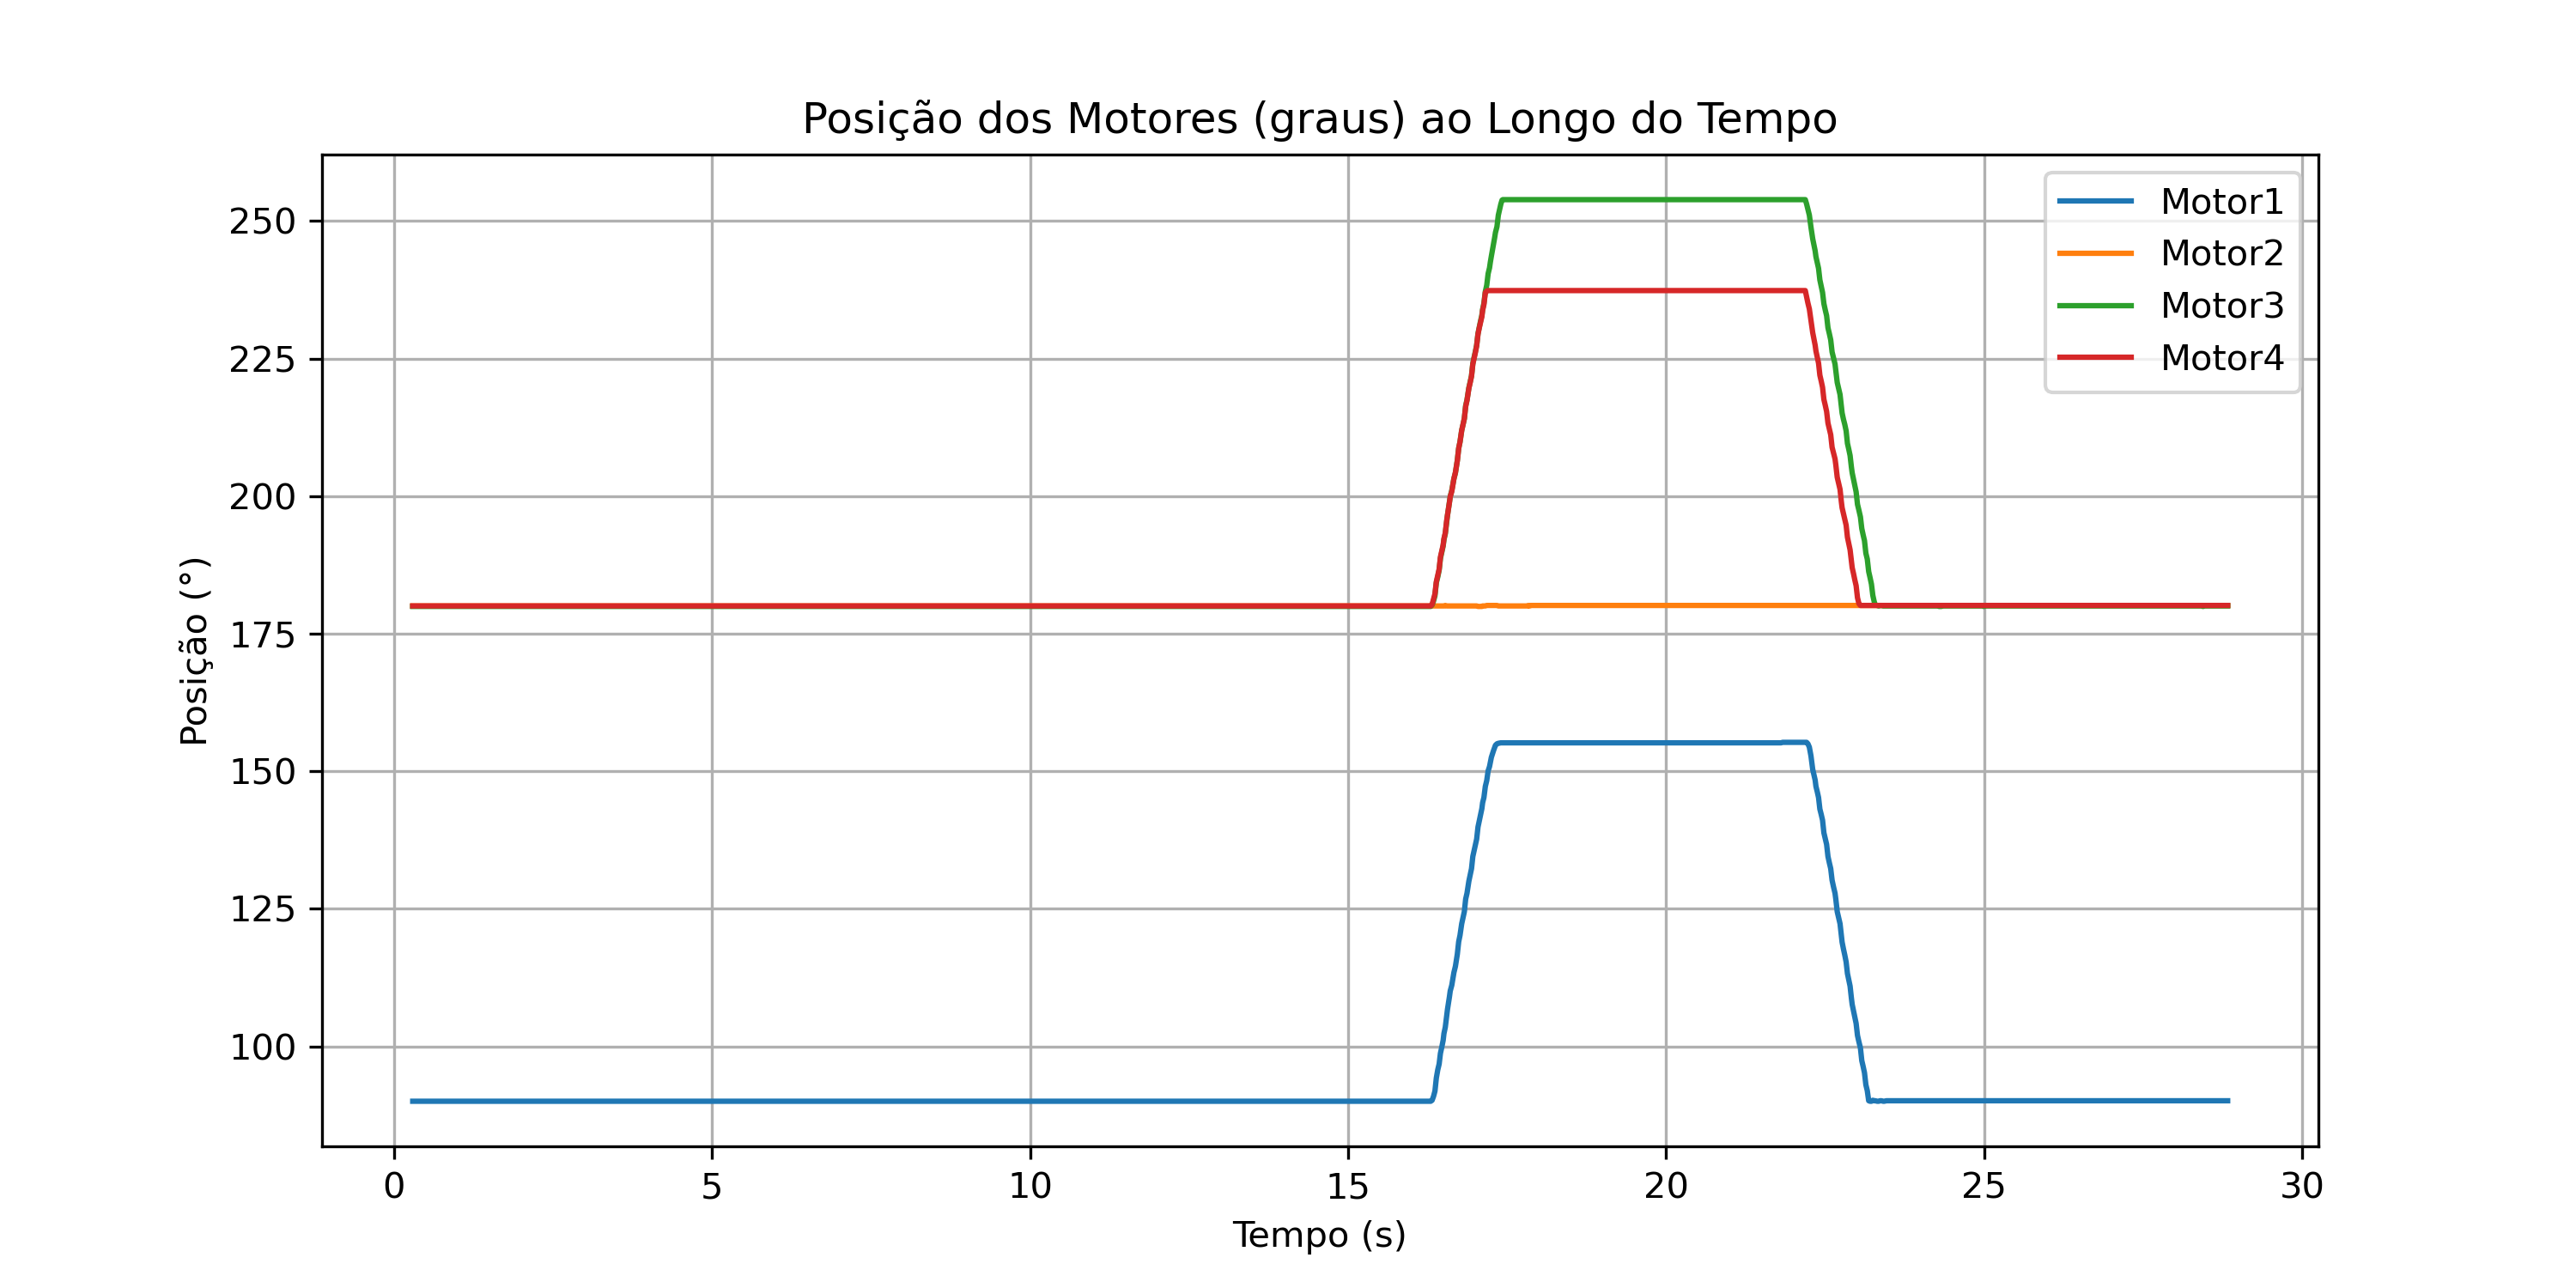
\includegraphics[width=0.33\textwidth]{figs/appendix/teste_pos_obst/finger_pos_vel50_obs_motor1.png} &
  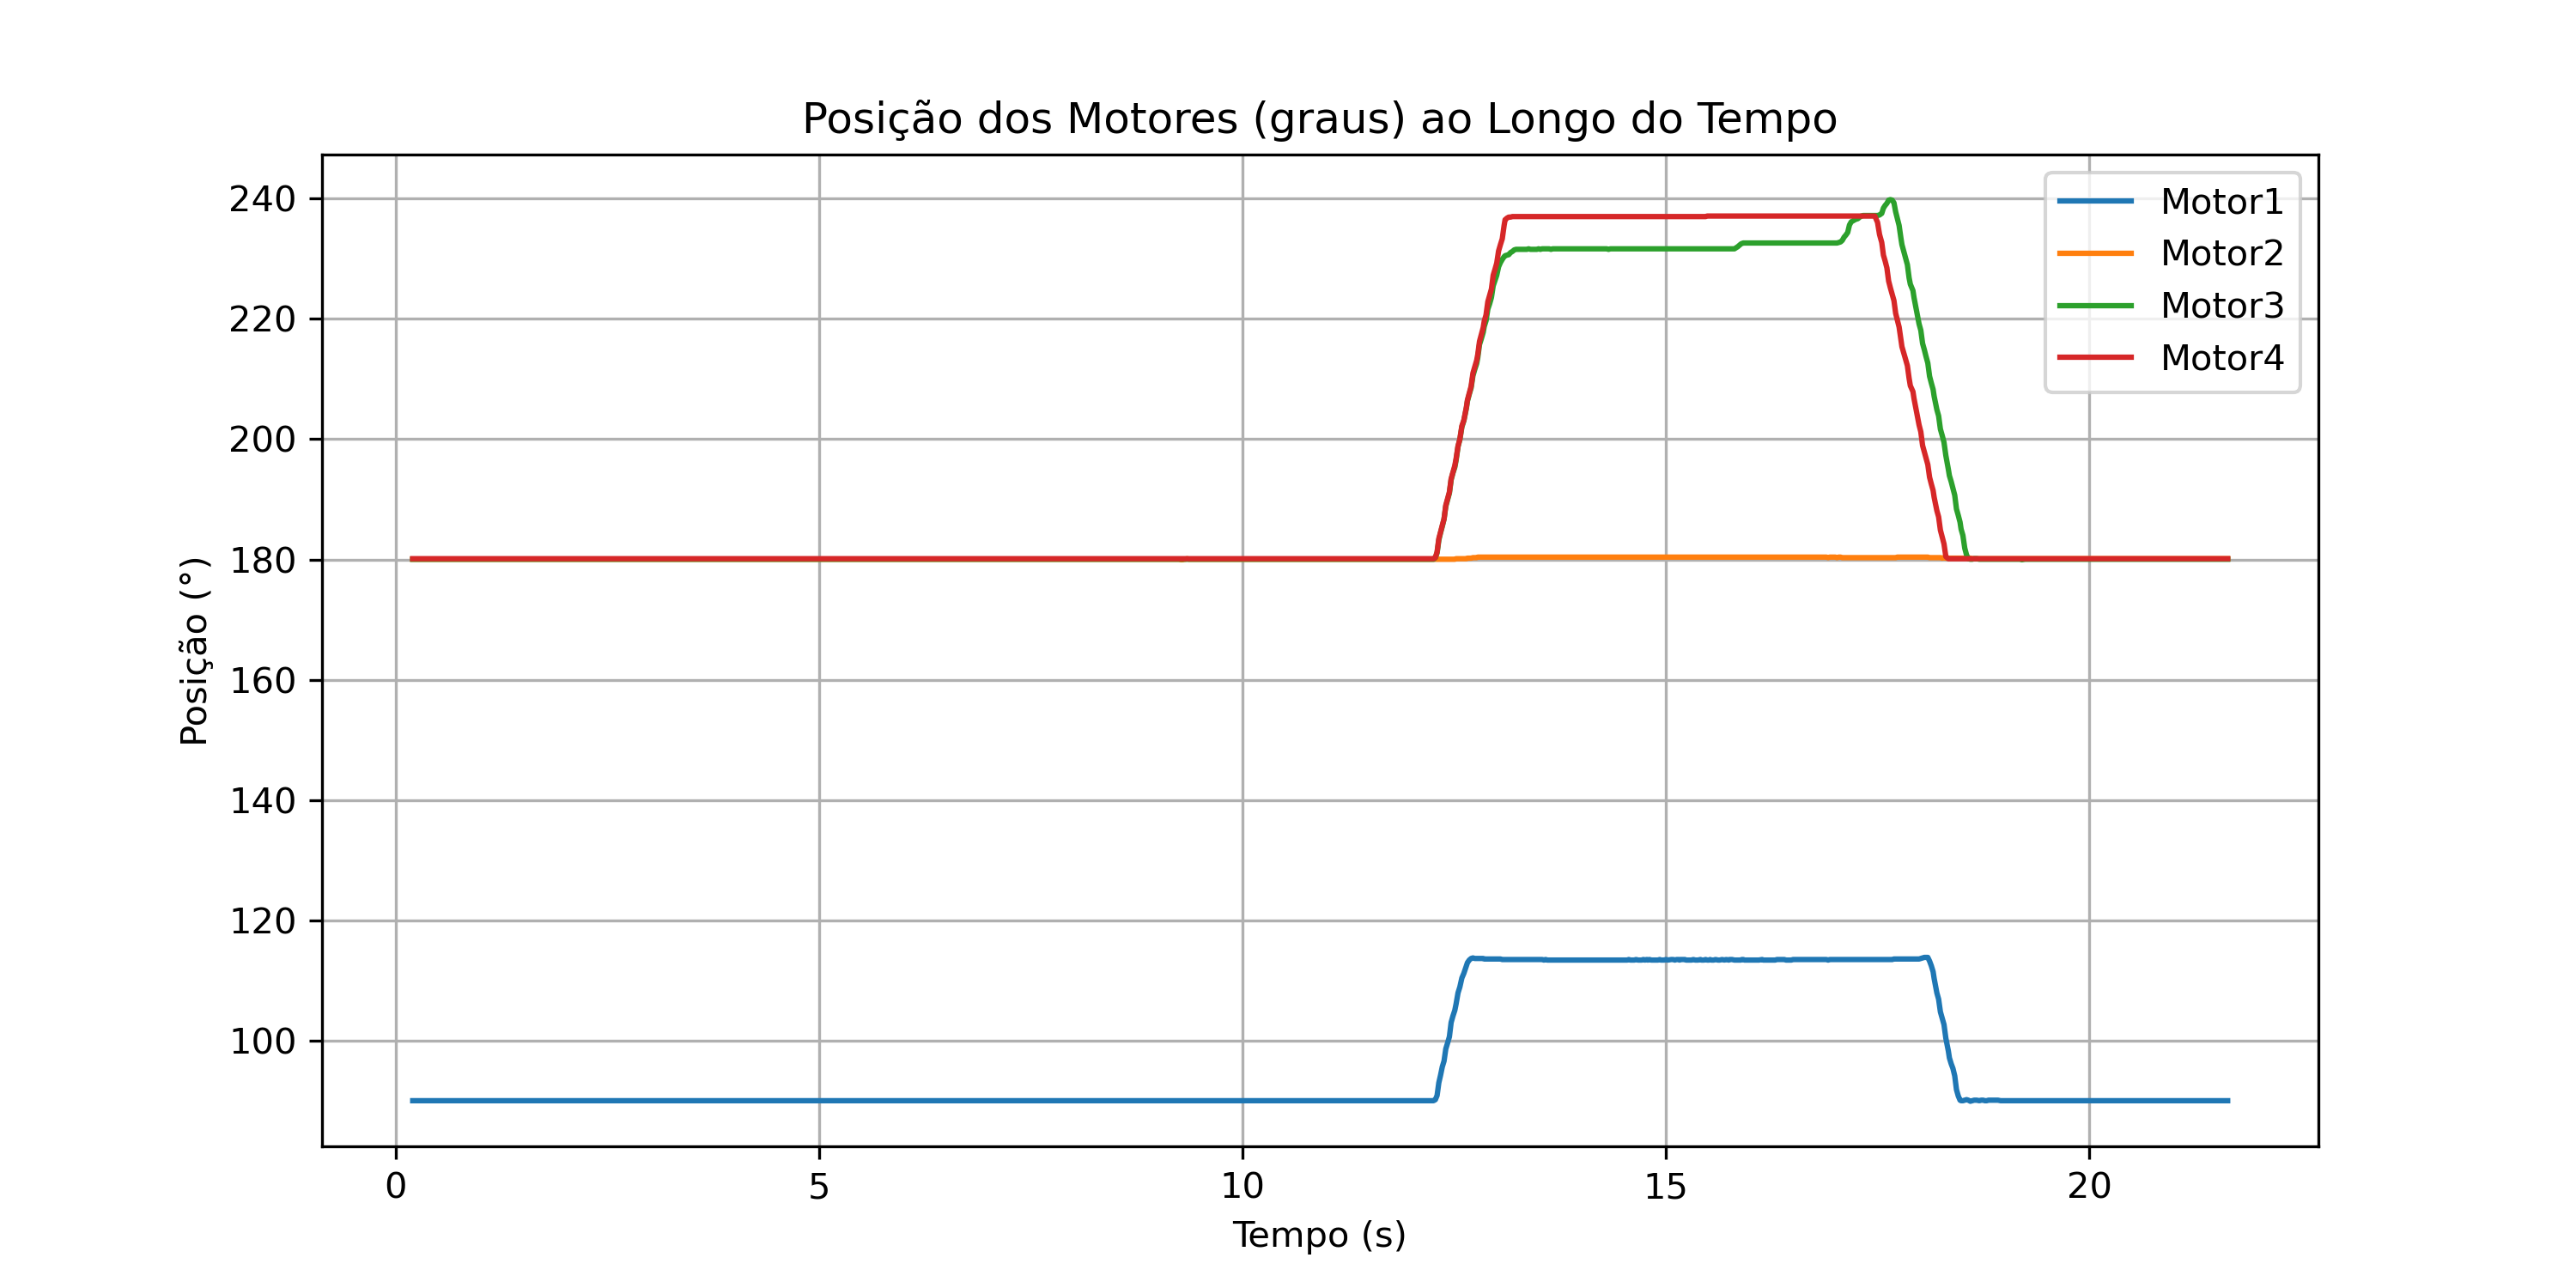
\includegraphics[width=0.33\textwidth]{figs/appendix/teste_pos_obst/finger_pos_vel50_obs_motor2.png} &
  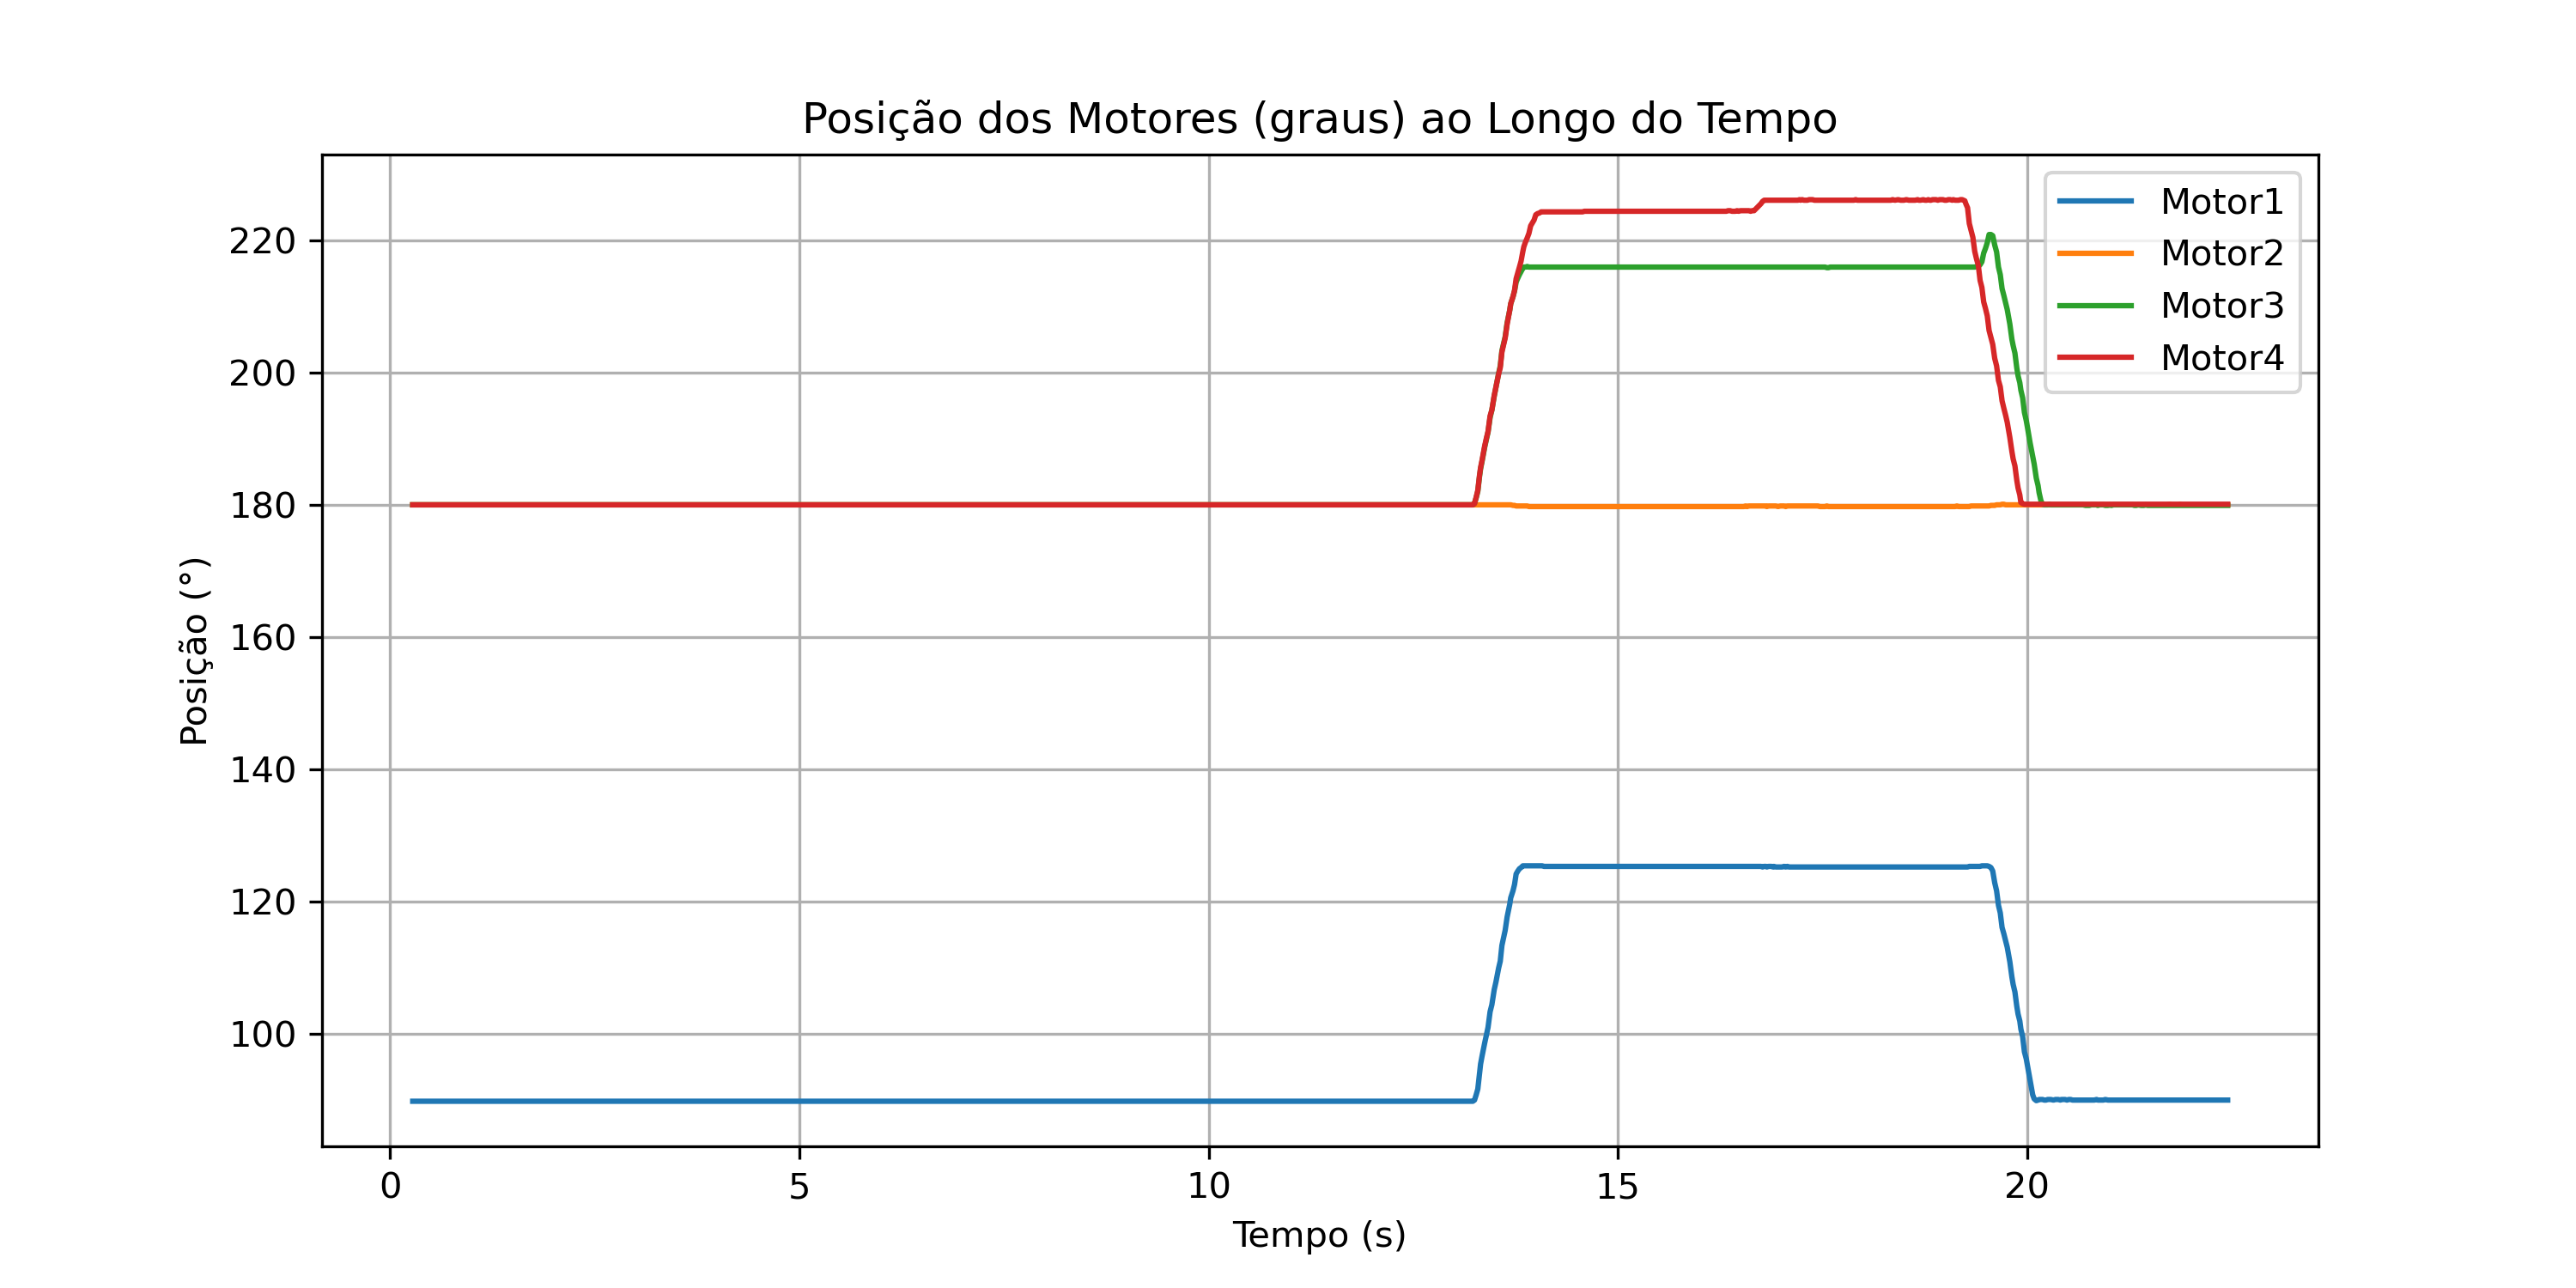
\includegraphics[width=0.33\textwidth]{figs/appendix/teste_pos_obst/finger_pos_vel50_obs_ponta.png} \\
  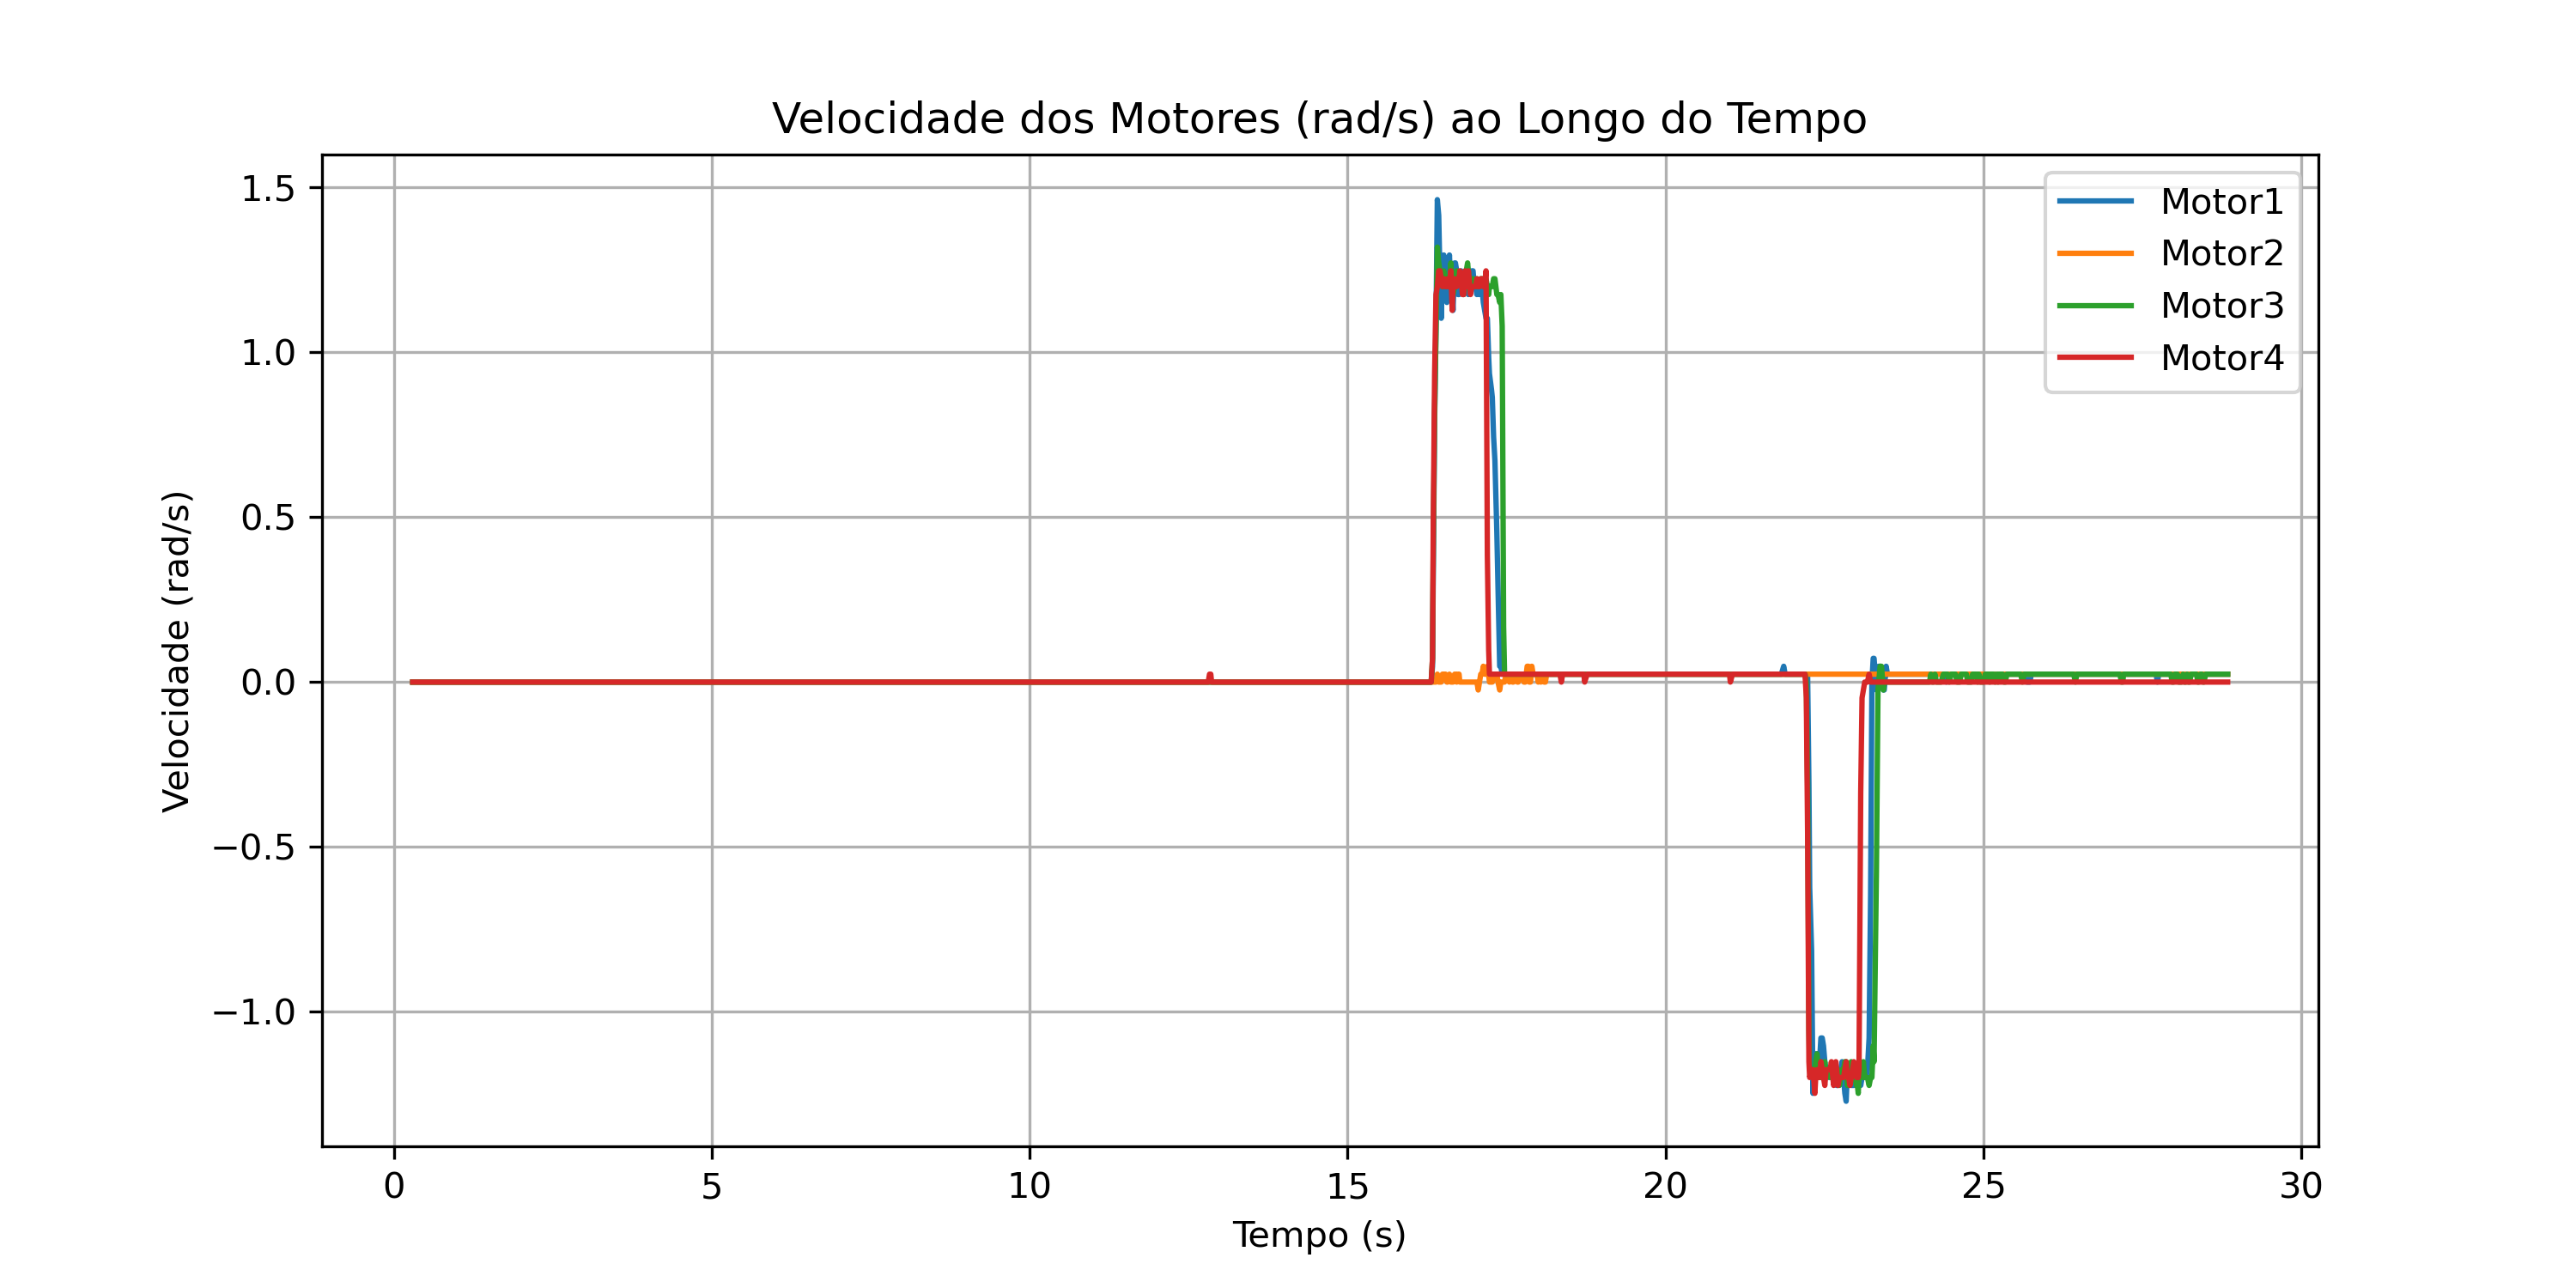
\includegraphics[width=0.33\textwidth]{figs/appendix/teste_pos_obst/finger_vels_vel50_obs_motor1.png} &
  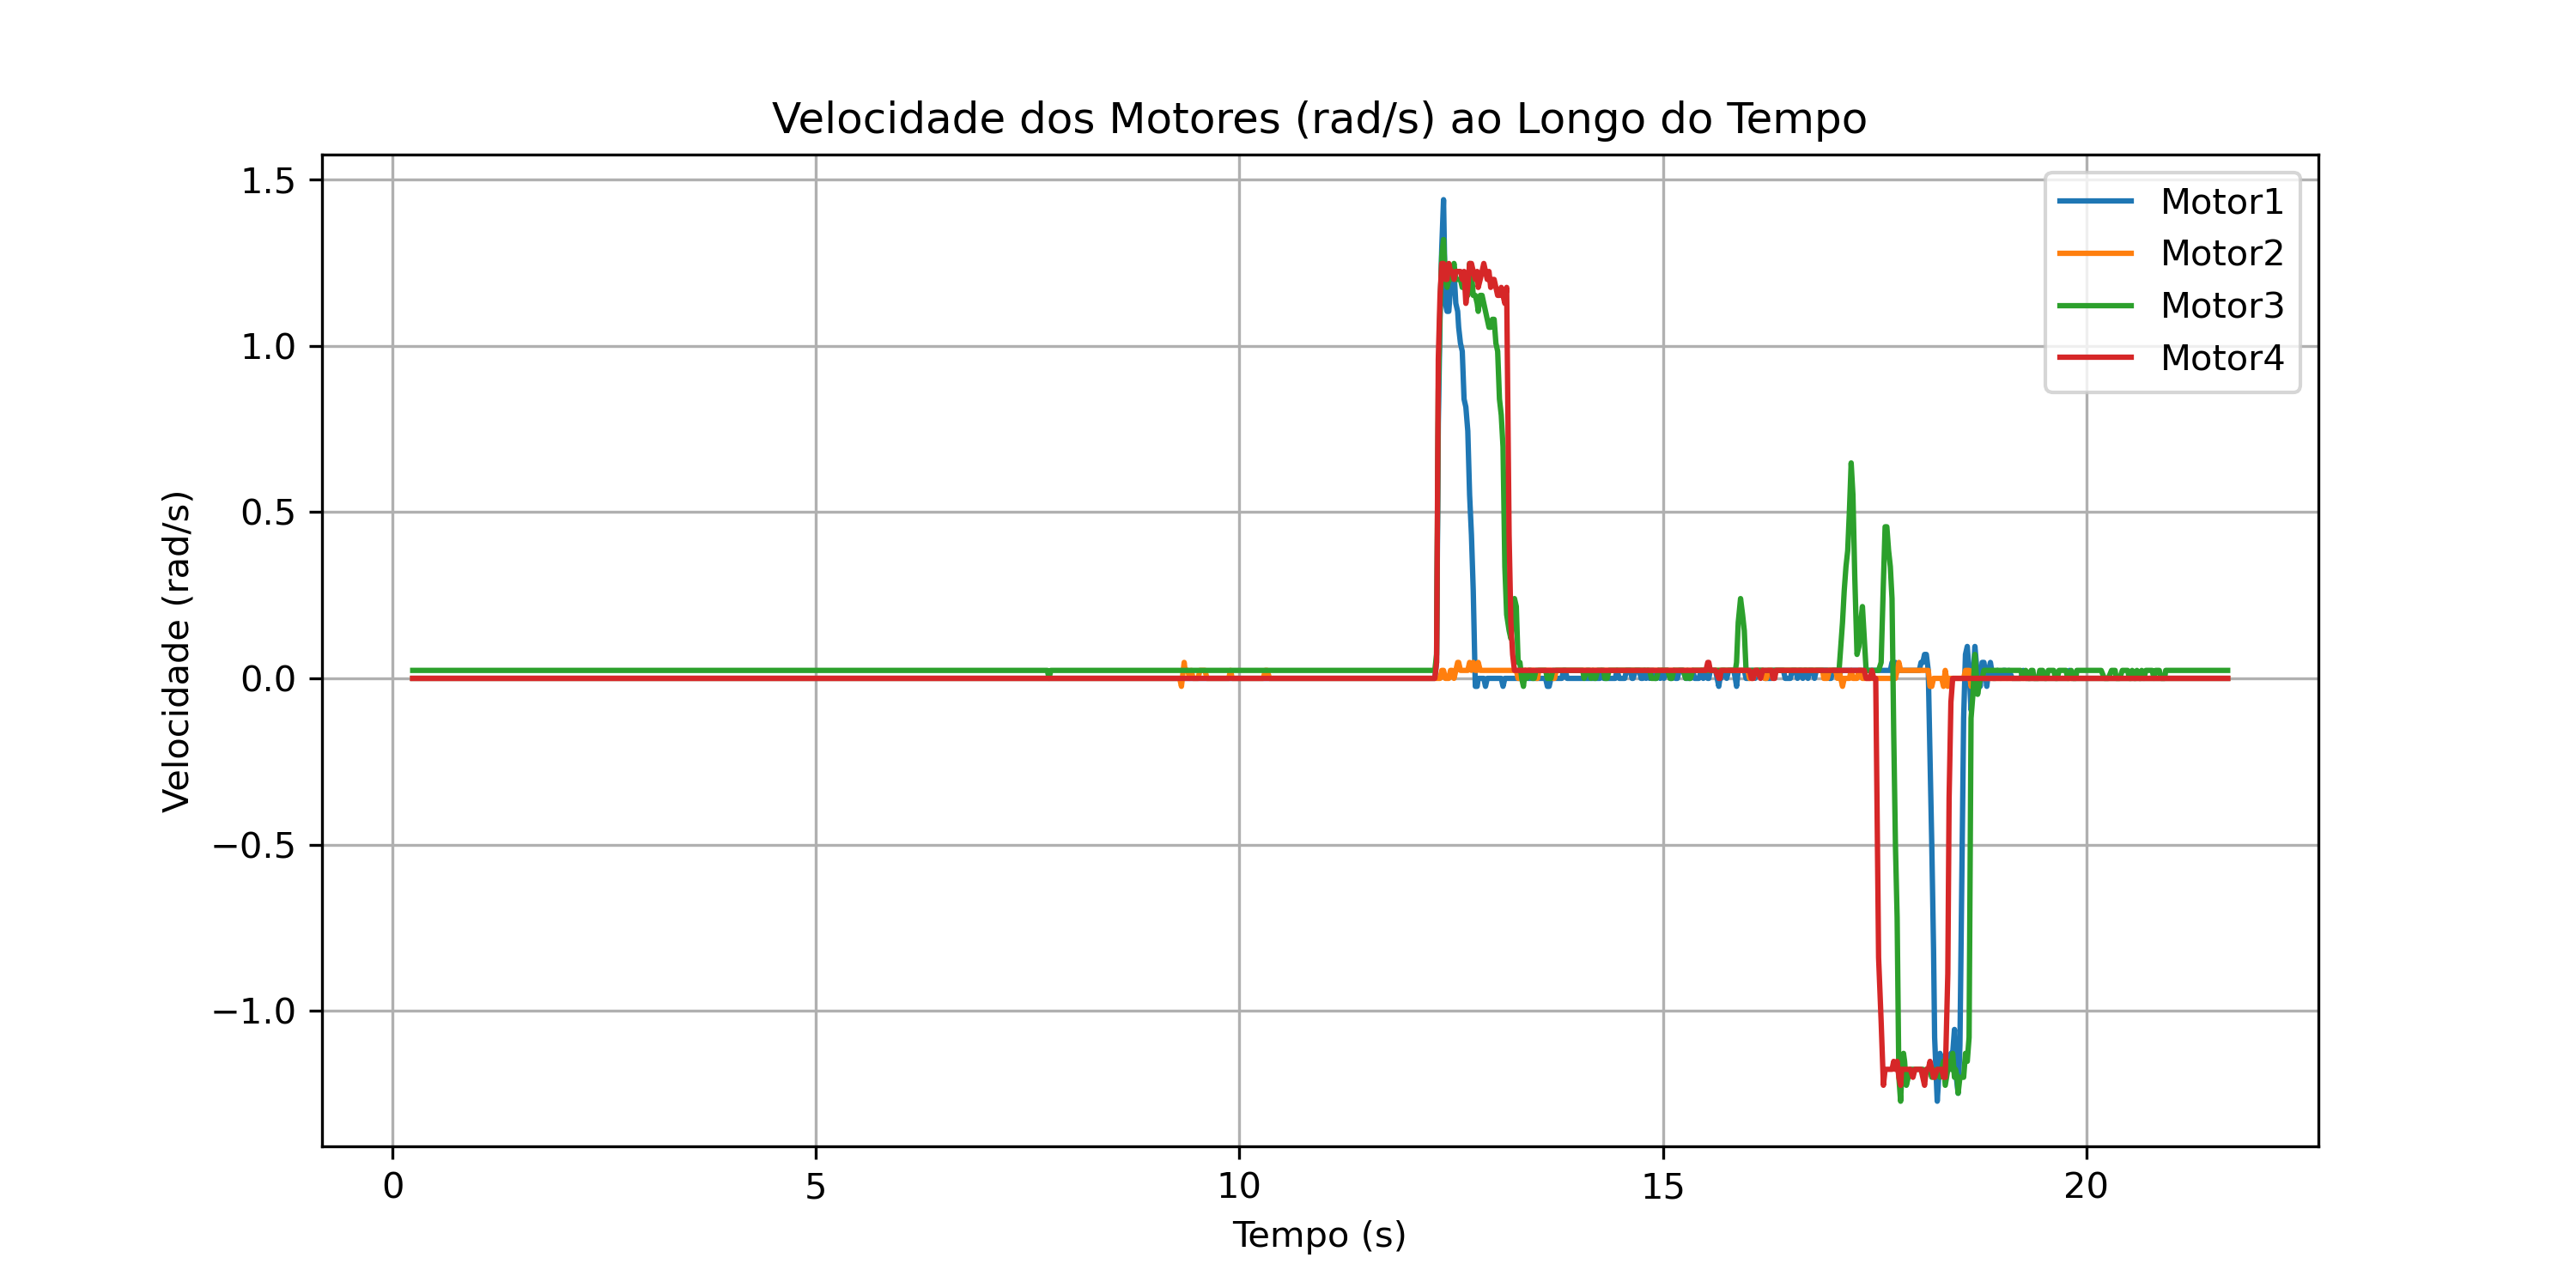
\includegraphics[width=0.33\textwidth]{figs/appendix/teste_pos_obst/finger_vels_vel50_obs_motor2.png} &
  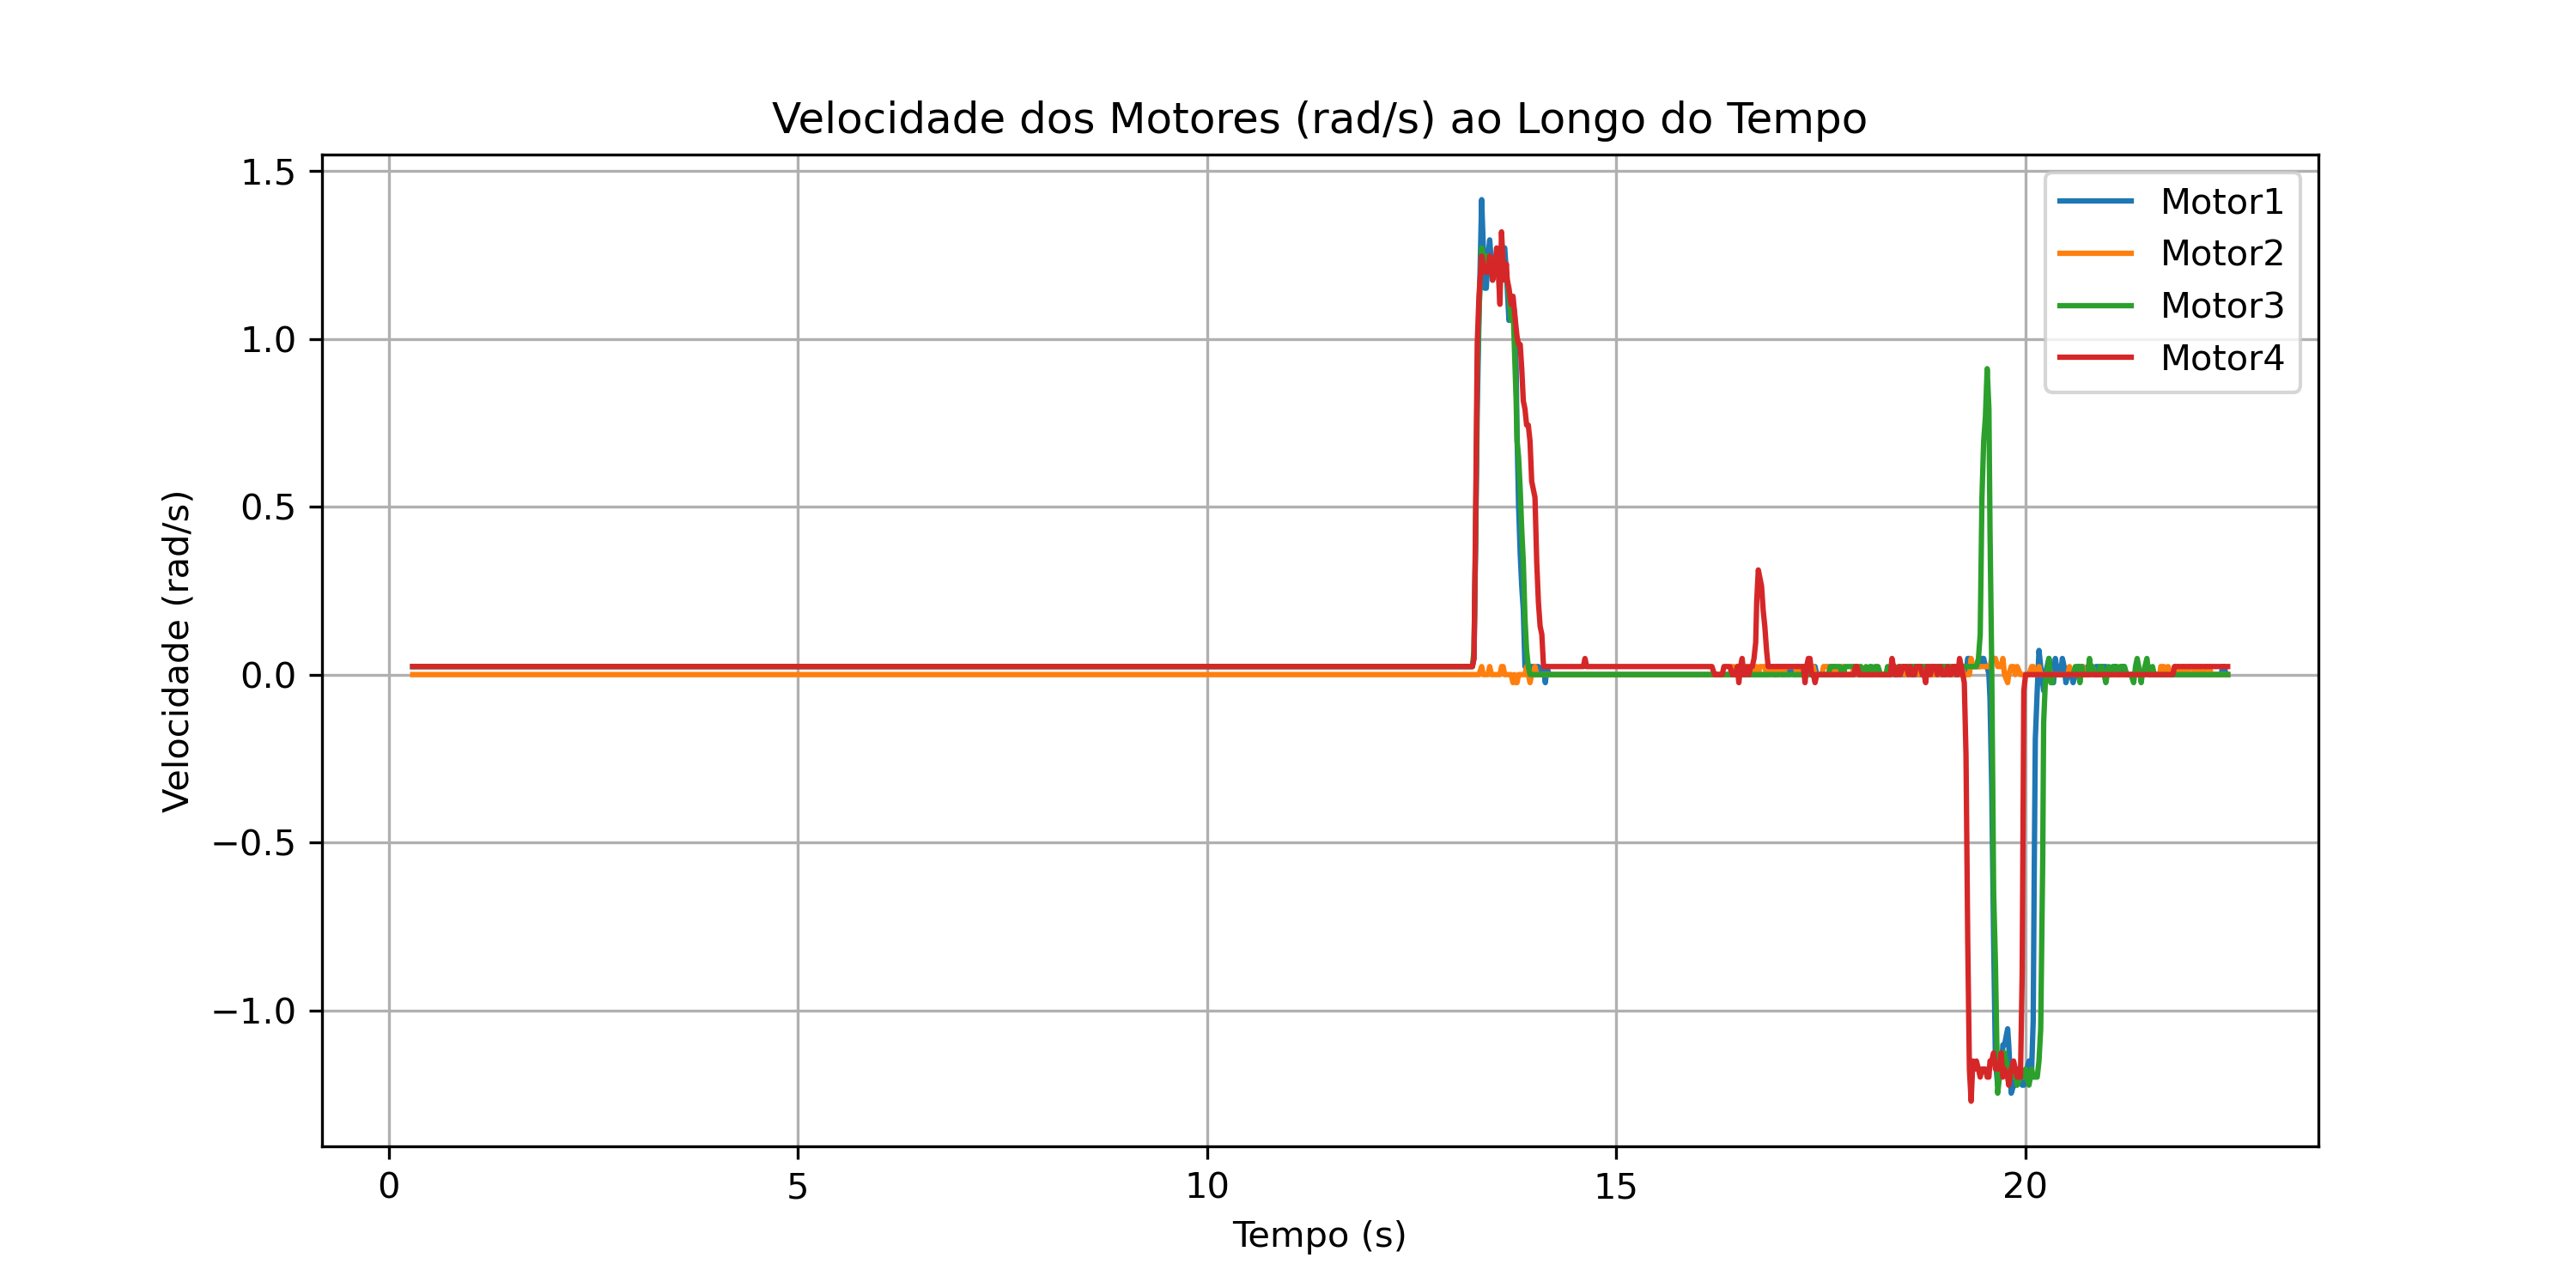
\includegraphics[width=0.33\textwidth]{figs/appendix/teste_pos_obst/finger_vels_vel50_obs_ponta.png} \\
  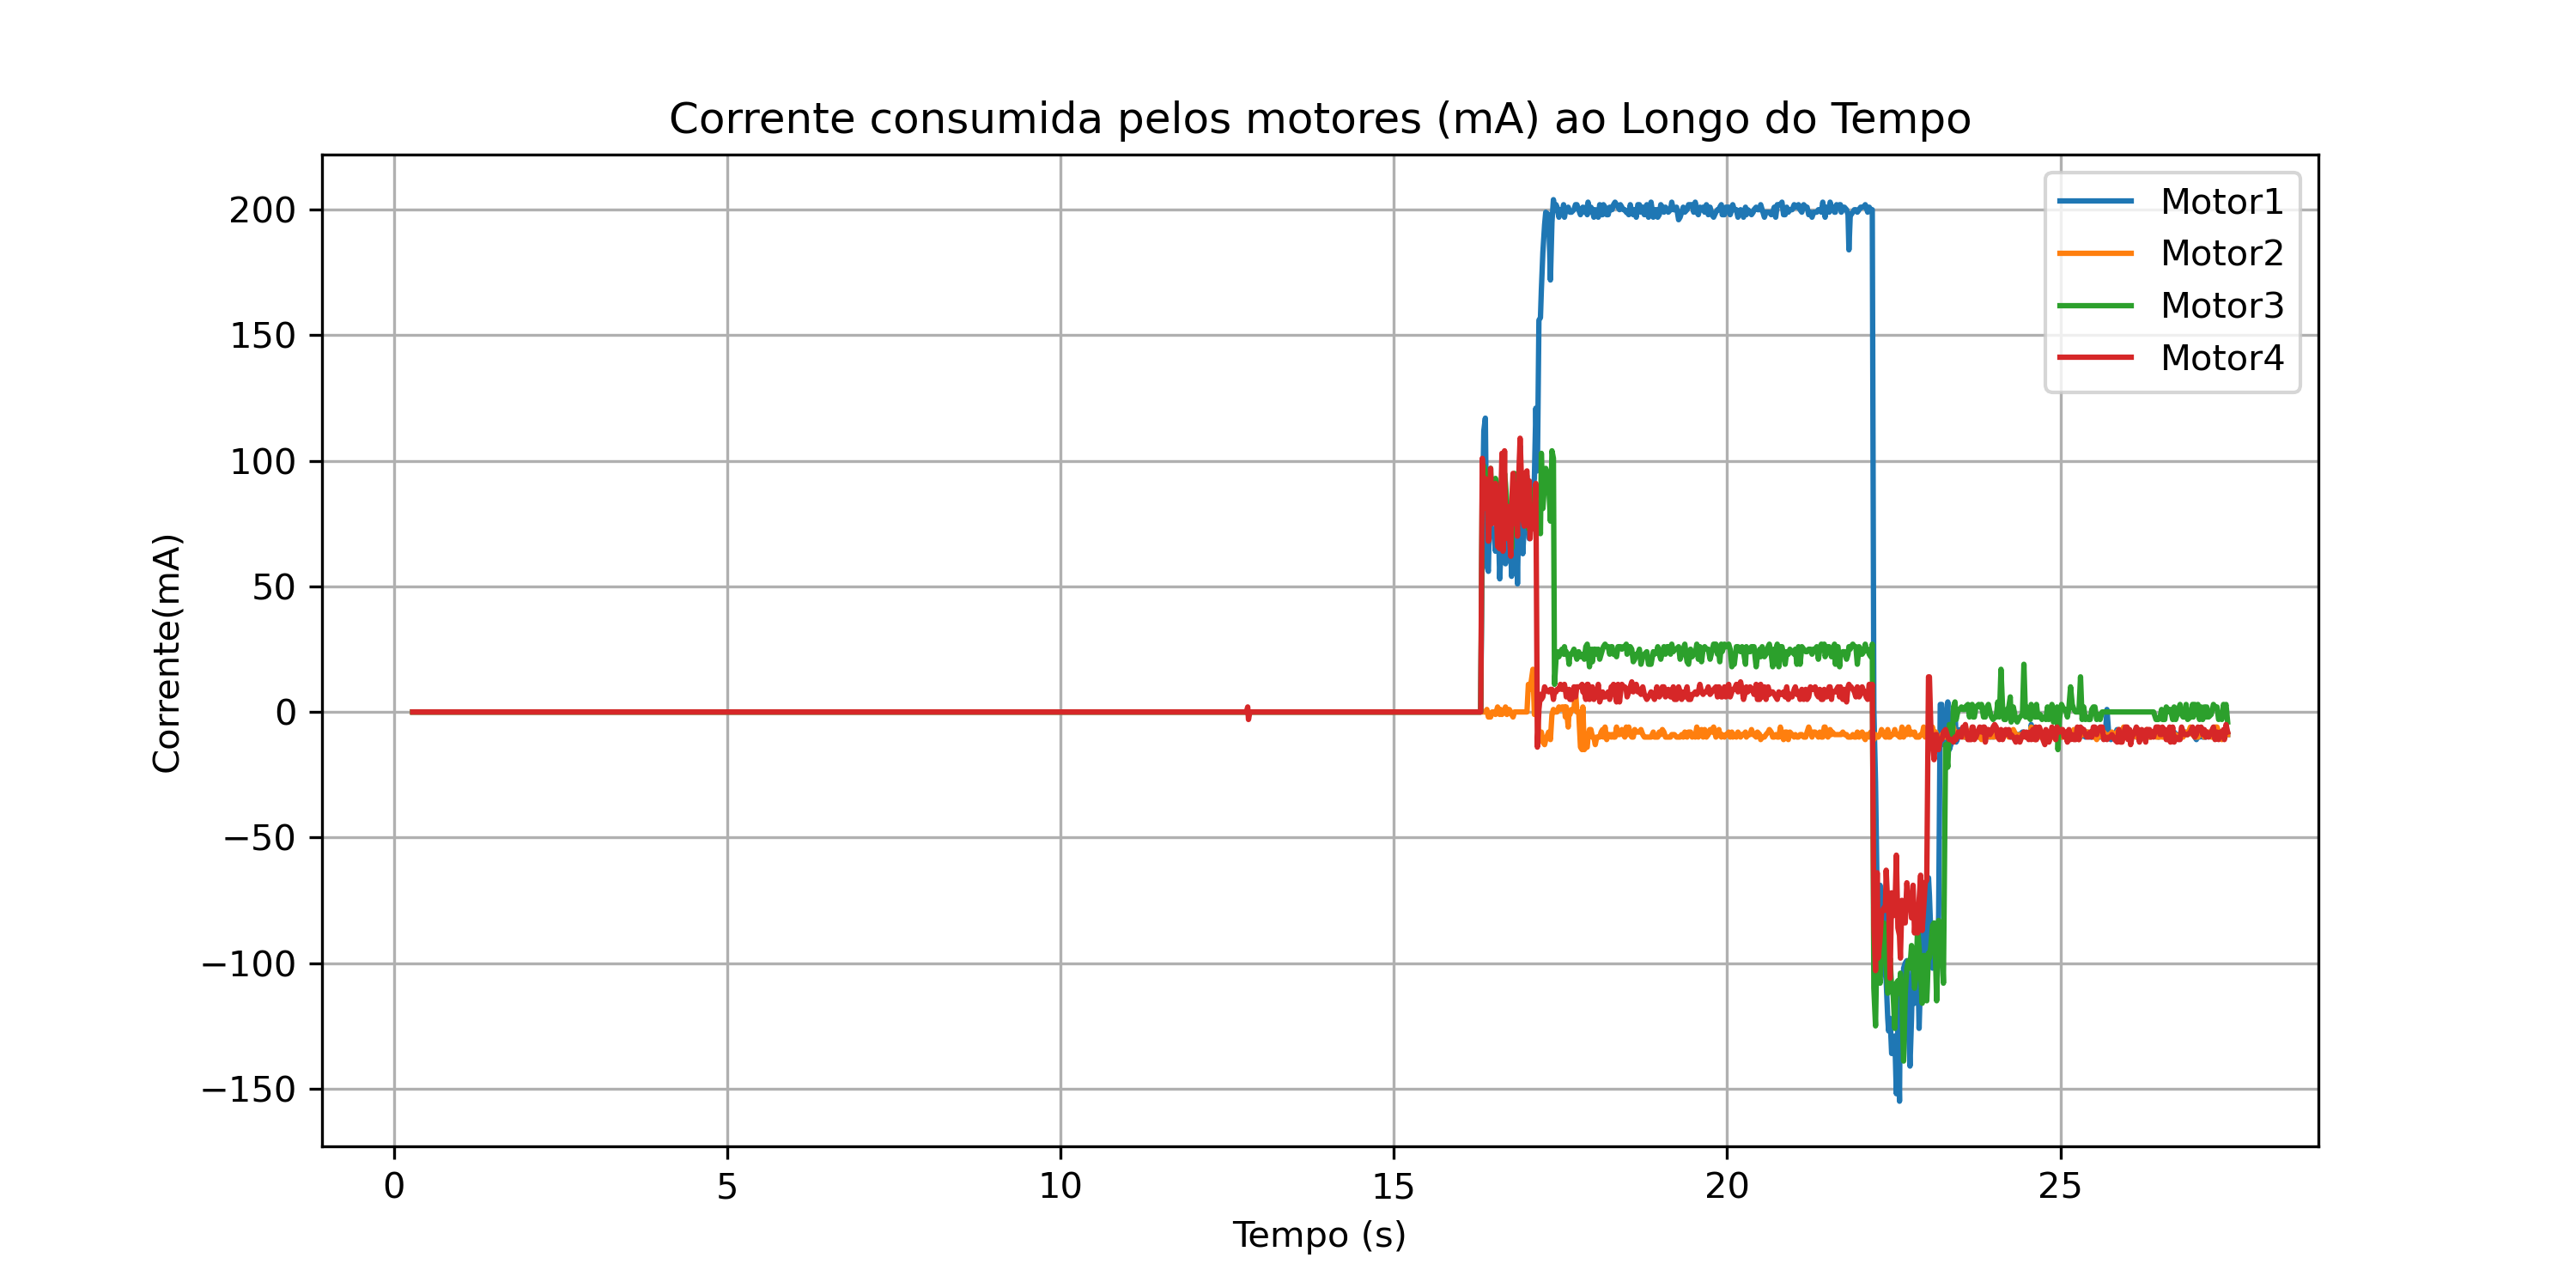
\includegraphics[width=0.33\textwidth]{figs/appendix/teste_pos_obst/finger_currs_vel50_obs_motor1.png} &
  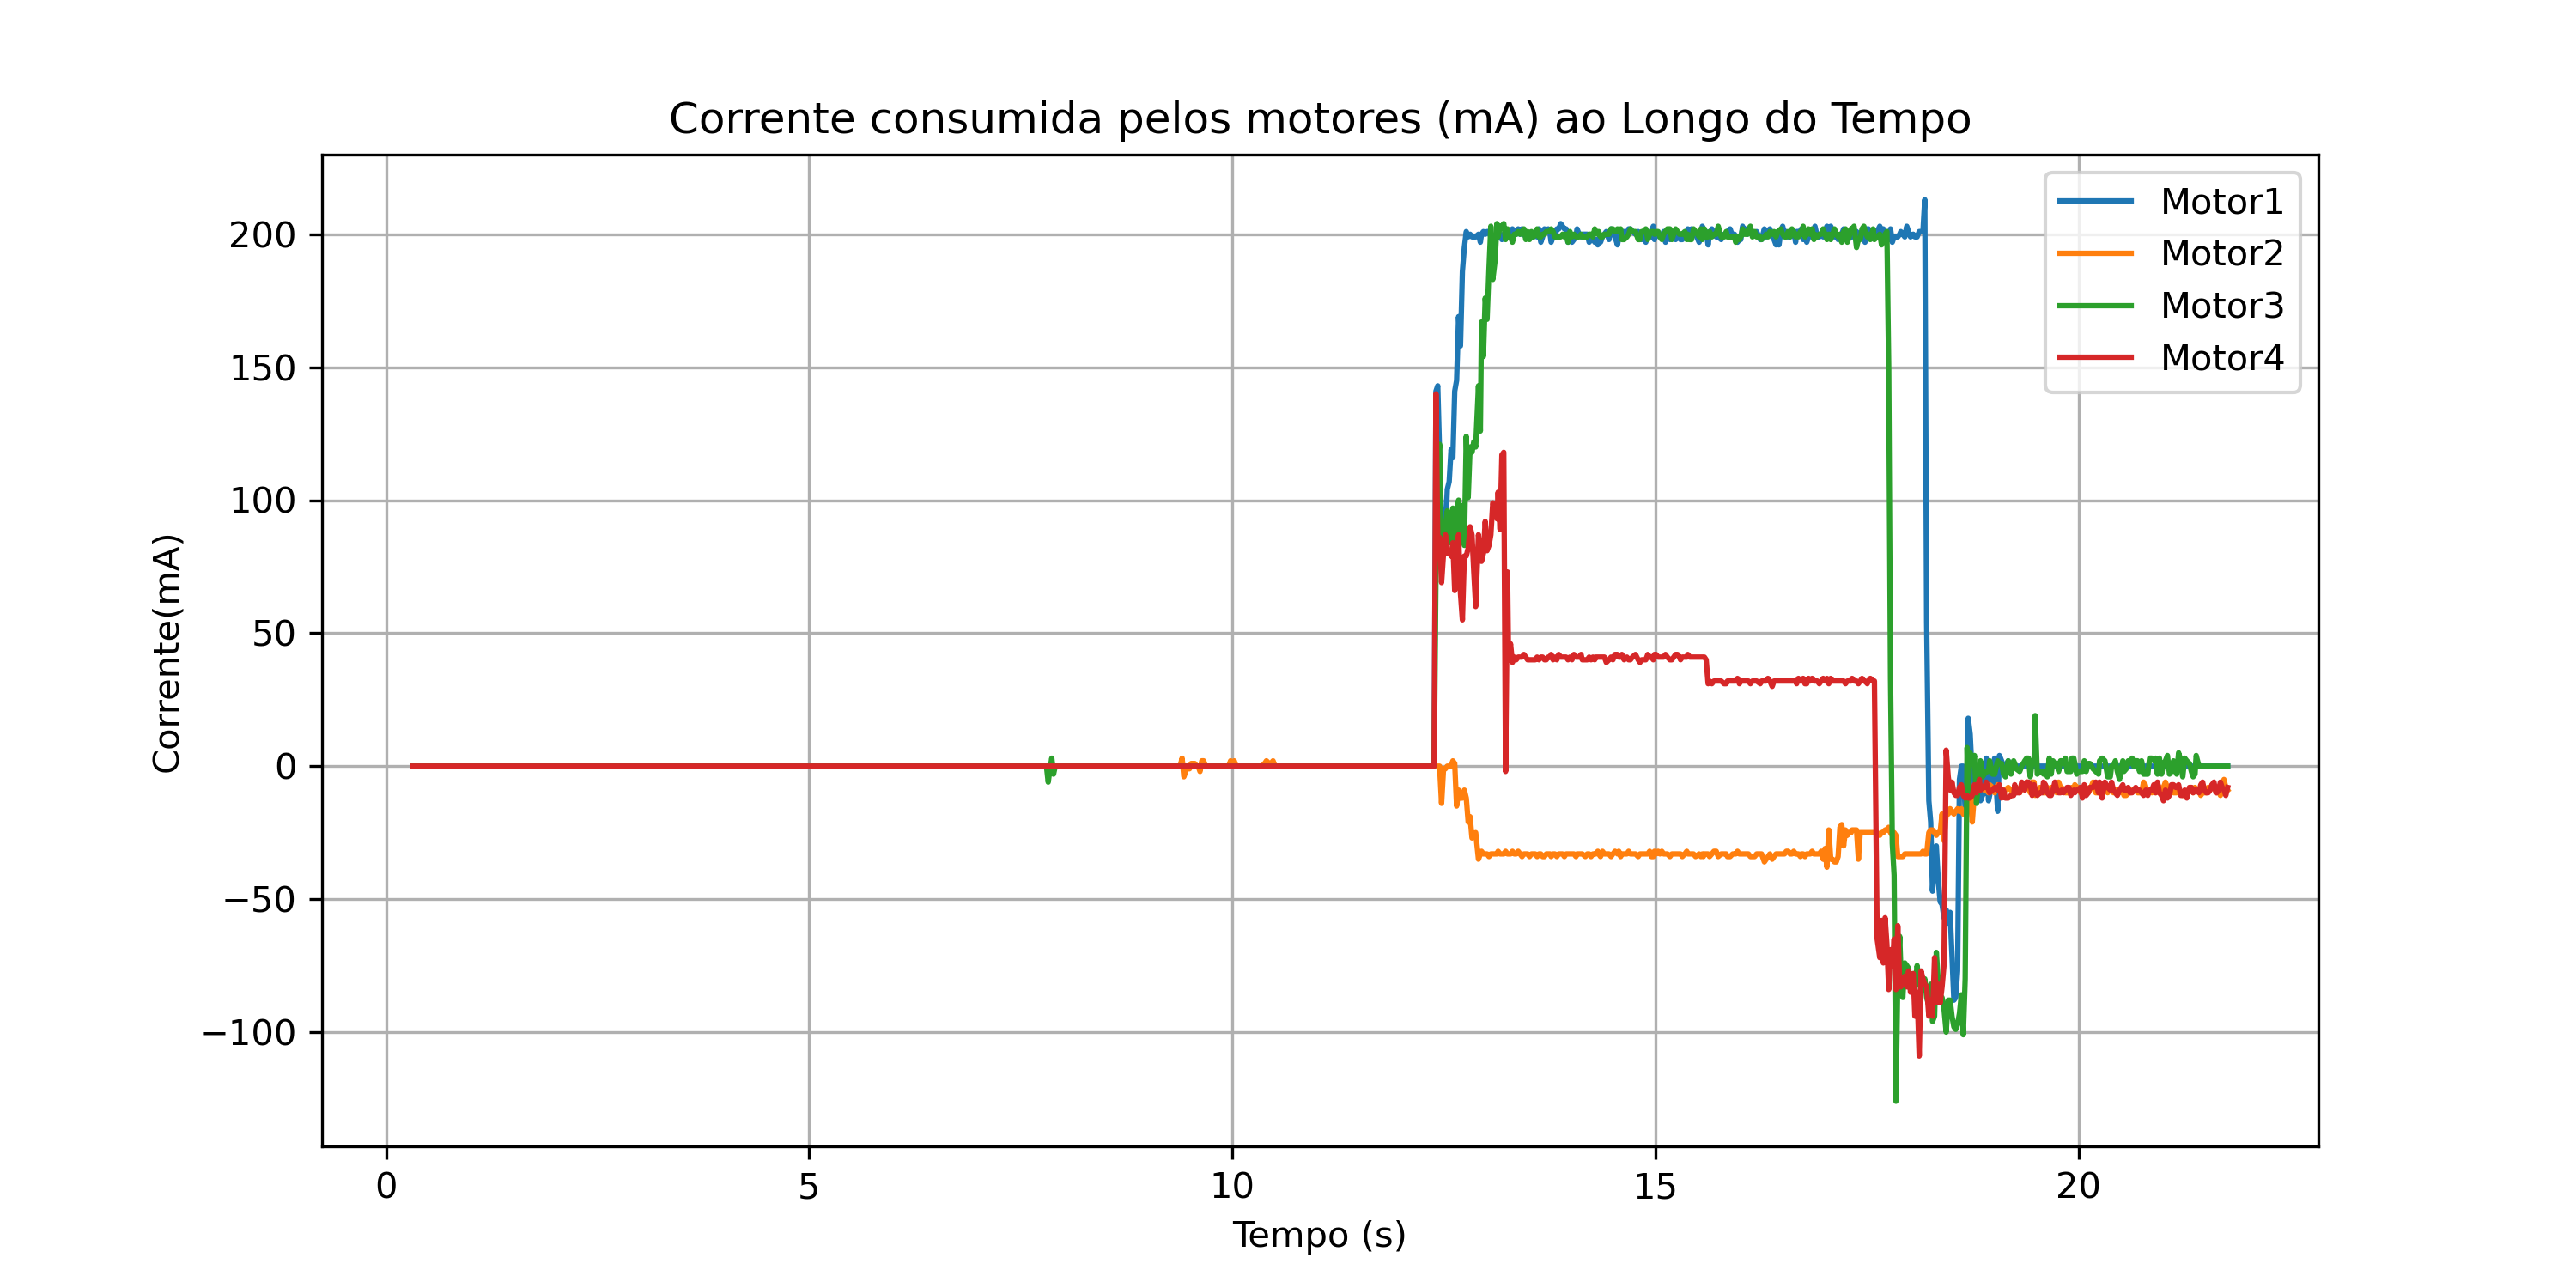
\includegraphics[width=0.33\textwidth]{figs/appendix/teste_pos_obst/finger_currs_vel50_obs_motor2.png} &
  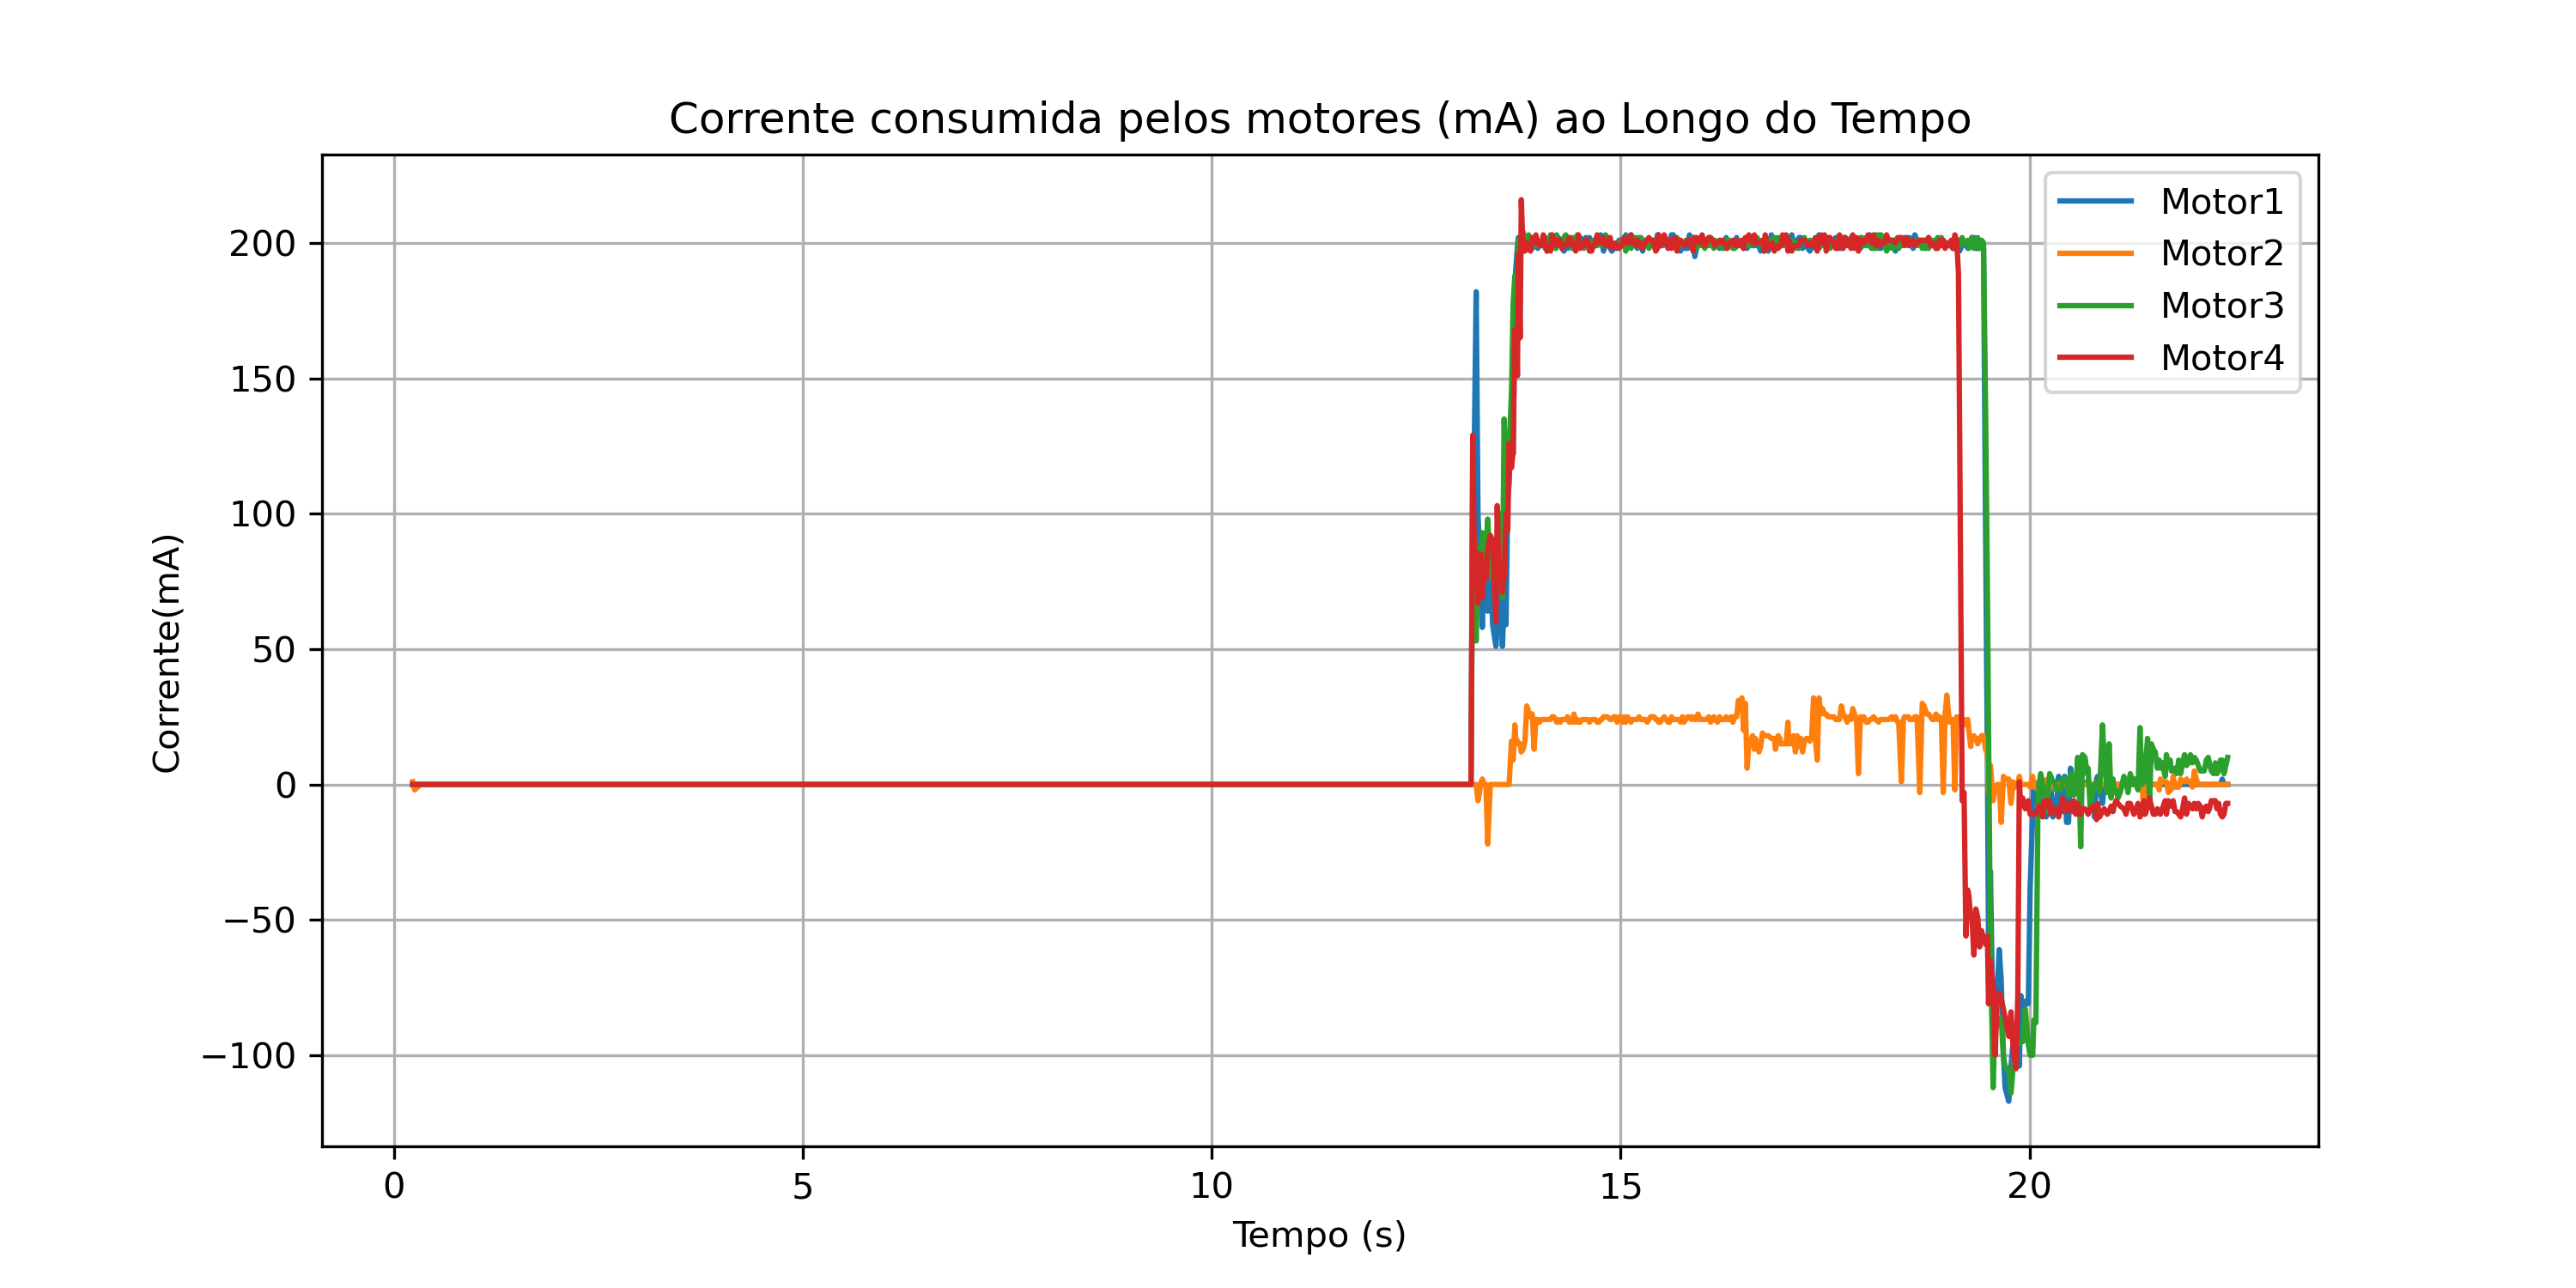
\includegraphics[width=0.33\textwidth]{figs/appendix/teste_pos_obst/finger_currs_vel50_obs_ponta.png} \\
\end{tabular}
\caption{Gráficos da posição, velocidade e corrente consumida pelos motores de um dedo, em diferentes cenários de obstrução. A coluna da esquerda representa a presença de um obstáculo junto ao motor mais próximo da base do dedo, a coluna central refere-se à obstrução a meio do dedo, e a coluna da direita corresponde à interferência na ponta do dedo.}
\end{figure}

Hiperligação para vídeo: \url{https://www.youtube.com/shorts/Qy4lXXRUP4Q}

\label{appendix:teste_posições_obstaculos}
